%%%%%%%%%%%%%%%%%%%%%%%%%%%%%%%%%%%%%%%%%%%%%%%%%%%%%%%%%%%%%%%%%%%
%                                                                 %
%  GEANT manual in LaTeX form                                     %
%                                                                 %
%  Version 1.00                                                   %
%                                                                 %
%  Last Mod. 8 June 1993  17:20  MG                               %
%                                                                 %
%%%%%%%%%%%%%%%%%%%%%%%%%%%%%%%%%%%%%%%%%%%%%%%%%%%%%%%%%%%%%%%%%%%
\documentstyle[11pt,fleqn,epsfig,crngeant,bibunits,fontcmds,multicol]{cernman}
\newcommand{\Title}{GEANT User's Guide}%           Title for document
\psfigdriver{DVIPS}
\makeindex
\romanfont{times}
\PScommands% Initialize PS boxes
\newmathalphabet*{\mathtt}{cmtt}{m}{n}
\newmathalphabet*{\mathbf}{cmr}{b}{n}
\begin{document}
%  ==================== Front material ============================
%%%%%%%%%%%%%%%%%%%%%%%%%%%%%%%%%%%%%%%%%%%%%%%%%%%%%%%%%%%%%%%%%%%
%                                                                 %
%   GEANT -- Short write ups -- LaTeX Source                      %
%                                                                 %
%   Front Material: Title page,                                   %
%                   Copyright Notice                              %
%                   Preliminary Remarks                           %
%                   Table of Contents                             %
%   EPS file      : cern15.eps, cnastit.eps                       %
%                                                                 %
%   Editor: Michel Goossens / CN-AS                               %
%   Last Mod.: 11 June 1993 10:30 mg                              %
%                                                                 %
%%%%%%%%%%%%%%%%%%%%%%%%%%%%%%%%%%%%%%%%%%%%%%%%%%%%%%%%%%%%%%%%%%%
 
%%%%%%%%%%%%%%%%%%%%%%%%%%%%%%%%%%%%%%%%%%%%%%%%%%%%%%%%%%%%%%%%%%%%
%    Tile page                                                     %
%%%%%%%%%%%%%%%%%%%%%%%%%%%%%%%%%%%%%%%%%%%%%%%%%%%%%%%%%%%%%%%%%%%%
\latex{\def\Ptitle#1{\special{ps: /Printstring (#1) def}
                       \epsfbox{eps/cnastit.eps}}}
 
\begin{titlepage}
%begin{latexonly}
\vspace*{-23mm}%
\includegraphics[height=30mm]{cern.eps}
\hfill
\raise8mm\hbox{\Large\bf CERN Program Library Long Writeup W5013}
\hfill\mbox{}
\begin{center}
\mbox{}\\[6mm]
\mbox{\Ptitle{GEANT}}\\[3cm]
{\Huge Detector Description and}\\[2cm]
{\Huge Simulation Tool}\\[4cm]
{\Large Application Software Group}\\[6mm]
{\Large Computing and Networks Division}\\[2cm]
\end{center}
\vfill
\begin{center}\Large CERN Geneva, Switzerland\end{center}
%end{latexonly}
\begin{htmlonly}
\begin{center}
\Large CERN Program Library Long Writeup W5013\\[1cm]
\Huge GEANT\\[2cm]
\Large Detector Description and Simulation Tool\\[1cm]
\large IT/ASD Group\\
\large CERN, Geneva, Switzerland
\end{center}
\end{htmlonly}
\end{titlepage}

%%%%%%%%%%%%%%%%%%%%%%%%%%%%%%%%%%%%%%%%%%%%%%%%%%%%%%%%%%%%%%%%%%%%
%    Copyright  page                                               %
%%%%%%%%%%%%%%%%%%%%%%%%%%%%%%%%%%%%%%%%%%%%%%%%%%%%%%%%%%%%%%%%%%%%

\thispagestyle{empty}
\framebox[\textwidth][t]{\hfill\begin{minipage}{0.96\textwidth}%
\vspace*{3mm}
\begin{center}Copyright Notice\end{center}
\parskip\baselineskip

\textbf{GEANT -- Detector Description and Simulation Tool}
 
\copyright{} Copyright CERN, Geneva 1993
 
Copyright and any other appropriate legal protection of these
computer programs and associated documentation reserved in all
countries of the world.
 
These programs or documentation may not be reproduced by any
method without prior written consent of the Director-General
of CERN or his delegate.
 
Permission for the usage of any programs described herein is
granted apriori to those scientific institutes associated with
the CERN experimental program or with whom CERN has concluded
a scientific collaboration agreement.
 
CERN welcomes comments concerning the Geant code
but undertakes no obligation for the maintenance of the programs,
nor responsibility for their correctness, and accepts no liability
whatsoever resulting from the use of its programs.
 
Requests for information should be addressed to:
\vspace*{-.5\baselineskip}
\begin{center}\ttfamily
\begin{tabular}{l}
CERN Program Library Office              \\
CERN-IT Division                         \\
CH-1211 Geneva 23                        \\
Switzerland                              \\
Tel.      +41 22 767 4951                \\
Fax.      +41 22 767 7155                \\
Email:    cernlib@cern.ch                \\
WWW:      http://wwwinfo.cern.ch/asd/index.html
\end{tabular}
\end{center}
\vspace*{2mm}
\end{minipage}\hfill}%end of minipage in framebox
\vspace{6mm}
 
{\bf Trademark notice: All trademarks appearing in this guide are acknowledged as such.}
\vfill

\begin{tabular}{l@{\quad}l@{\quad}>{\small\ttfamily}l}
\emph{Contact Persons}:       & IT/ASD/SImulation section & (giani\atsign cern.ch)\\[1mm]
\emph{Documentation Consultant}: & Michel Goossens /IT    & (goossens\atsign cern.ch)\\[1cm]
\textem{Edition -- March 1994}
\end{tabular}
\newpage
 

%  ==================== Body of text ==============================
\pagenumbering{arabic}
\setcounter{page}{1}
 
%%%%%%   Catalog of Program packages and entries%%%%
 
\def\Rtnr{Catalog}%Dummy routine name to appear at bottom of page
%%%%%%%%%%%%%%%%%%%%%%%%%%%%%%%%%%%%%%%%%%%%%%%%%%%%%%%%%%%%%%%%%%%
%                                                                 %
%  GEANT manual in LaTeX form   	                          %
%                                                                 %
%  Michel Goossens (for translation into LaTeX)                   %
%  Version 2.00                                                   %
%  Last Mod.  2 Jun 1998  17:10   MG                              %
%                                                                 %
%%%%%%%%%%%%%%%%%%%%%%%%%%%%%%%%%%%%%%%%%%%%%%%%%%%%%%%%%%%%%%%%%%%
%%% Generated from headings
\chapter{Catalog of Geant sections}
\begin{DLtt}{12345678}
\item[AAAA001] Foreword
\item[AAAA002] Introduction to the manual
\item[BASE001] Introduction to GEANT
\item[BASE010] Simplified Program Flow Chart
\item[BASE020] The data structures and their relationship
\item[BASE040] Summary of Data Records
\item[BASE090] The reference systems and physical units
\item[BASE100] Examples of GEANT application
\item[BASE110] The system initialisation routines
\item[BASE200] Steering routines for event processing
\item[BASE280] Storing and retrieving JRUNG and JHEAD information
\item[BASE299] The banks JRUNG and JHEAD
\item[BASE300] Example of user termination routine
\item[BASE400] Debugging facilities
\item[BASE410] Utility Routines
\item[BASE420] The random number generator
\item[CONS001] Introduction to the section CONS
\item[CONS100] Material definition
\item[CONS101] Retrieve material cross-sections and stopping power
\item[CONS110] Mixtures and Compounds
\item[CONS199] The Material data structure JMATE
\item[CONS200] Tracking medium parameters
\item[CONS210] Special Tracking Parameters
\item[CONS300] Particle definition
\item[CONS310] Branching Ratios and Particle Decay Modes
\item[DRAW001] Introduction to the Drawing package
\item[DRAW010] The Ray-tracing package
\item[DRAW110] Drawing a Volume -- Case 1
\item[DRAW115] Drawing a Volume Projection view -- Case 2
\item[DRAW120] Draw a volume cut view
\item[DRAW130] Draw Particle Trajectories
\item[DRAW140] Drawing Track Hits in Sensitive Detectors
\item[DRAW210] Drawing the geometrical tree
\item[DRAW220] Drawing volume specifications
\item[DRAW300] Handling View banks
\item[DRAW399] The data structure JDRAW
\item[DRAW400] Utility routines of the drawing package
\item[GEOM001] The geometry package
\item[GEOM010] Tracking inside volumes and optimisation
\item[GEOM020] ``MANY'' Volumes and boolean operations on volumes
\item[GEOM050] The GEANT shapes
\item[GEOM100] Creation of a volume
\item[GEOM110] Positioning a volume inside its mother
\item[GEOM120] Positioning a volume inside its mother with parameters
\item[GEOM130] Division of a volume into a given number of cells
\item[GEOM140] Division of a Volume into cells of a given size
\item[GEOM150] Division of a volume - general case
\item[GEOM199] The volume data structure -- JVOLUM
\item[GEOM200] Rotation matrices
\item[GEOM299] The rotation matrix data structure JROTM
\item[GEOM300] Finding in which volume a point is
\item[GEOM310] Finding distance to next boundary
\item[GEOM320] Reference system transformations
\item[GEOM400] Pseudo-division of a volume
\item[GEOM410] Ordering the contents of a volume
\item[GEOM500] Volume attributes
\item[GEOM600] User initialisation of the common block /GCVOLU/
\item[GEOM700] Medium search statistics
\item[GEOM900] End of geometry definition
\item[GEOM910] The CADINT Interface
\item[HITS001] The detector response package
\item[HITS100] Sensitive DETector definition
\item[HITS105] Detector aliases
\item[HITS110] DETector hit parameters
\item[HITS120] DETector Digitisation parameters
\item[HITS130] User detector parameters
\item[HITS199] The SET data structure JSET
\item[HITS200] Routines to store and retrieve HITS
\item[HITS299] The JHITS data structure
\item[HITS300] Routines to store and retrieve DIGItisations
\item[HITS399] The JDIGI data structure
\item[HITS400] Intersection of a track with a cylinder or a plane
\item[HITS500] Digitisation for drift- or MWP- Chambers
\item[HITS510] Digitisation for drift chambers
\item[IOPA001] The I/O routines
\item[IOPA200] ZEBRA sequential files handling
\item[IOPA300] Data structure I/O with sequential files
\item[IOPA400] ZEBRA direct access files handling
\item[IOPA500] Data structure I/O with direct access files
\item[KINE001] Section KINE
\item[KINE100] Storing and retrieving vertex and track parameters
\item[KINE199] The data structures JVERTX and JKINE
\item[KINE200] Interface to the Lund Monte Carlo
\item[KINE210] $\tau ^{\pm }$ generation and decay
\item[PHYS001] Introduction to the section PHYS
\item[PHYS010] Compute the occurrence of a process
\item[PHYS100] Steering routine for physics initialisation
\item[PHYS210] Total cross-section for e+e- pair production by photons
\item[PHYS211] Simulation of e-e+ pair production by photons
\item[PHYS220] Total cross-section for Compton scattering
\item[PHYS221] Simulation of Compton scattering
\item[PHYS230] Total cross-section for photoelectric effect
\item[PHYS231] Simulation of photoelectric Effect
\item[PHYS240] Photon-induced fission on heavy materials
\item[PHYS250] Total cross-section for Rayleigh scattering
\item[PHYS251] Simulation of Rayleigh scattering
\item[PHYS260] \v{C}erenkov photons
\item[PHYS320] Gaussian multiple scattering
\item[PHYS325] Moli\`ere scattering
\item[PHYS328] Plural scattering
\item[PHYS330] Ionisation processes induced by e+/e-
\item[PHYS331] Simulation of the delta-ray production
\item[PHYS332] Simulation of energy loss straggling
\item[PHYS333] Information about energy loss fluctuations
\item[PHYS334] Models for energy loss fluctuations in thin layers
\item[PHYS337] Birks' saturation law
\item[PHYS340] Total cross-section and energy loss for bremsstrahlung by e-e+
\item[PHYS341] Simulation of discrete bremsstrahlung by electrons
\item[PHYS350] Total cross-section for e+e- annihilation
\item[PHYS351] Simulation of e+e- annihilation
\item[PHYS360] Synchrotron radiation
\item[PHYS400] Simulation of particle decays in flight
\item[PHYS410] Rotations and Lorentz transformation
\item[PHYS430] Ionisation processes for muons and protons
\item[PHYS431] Ionisation processes for heavy ions
\item[PHYS440] Total cross-section and energy loss for bremsstrahlung by Muons
\item[PHYS441] Simulation of discrete bremsstrahlung by muons
\item[PHYS450] Total cross-section and energy loss for e-e+ pair production by muons
\item[PHYS451] Simulation of e+e- pair production by muons
\item[PHYS460] Muon-nucleus interactions
\item[PHYS510] The GEANT/GHEISHA Interface
\item[PHYS520] The GEANT/FLUKA Interface
\item[PHYS530] The GEANT/MICAP interface
\item[TRAK001] The tracking package
\item[TRAK110] Steering routine to track one event
\item[TRAK120] Steering routine to track one particle
\item[TRAK130] Tracking one particle through a volume
\item[TRAK200] The tracking routines block diagrams
\item[TRAK300] Storing secondary tracks in the stack
\item[TRAK310] Altering the order of tracking secondary particles
\item[TRAK399] The temporary stack data structure JSTAK
\item[TRAK400] Handling of track space points
\item[TRAK499] The space point data structure JXYZ
\item[TRAK500] Tracking routines in magnetic field
\item[XINT001] The interactive version of GEANT
\item[XINT002] Introduction to the Interactive version of GEANT
\item[XINT010] Screen views of GEANT++
\item[ZZZZ010] List of COMMON Blocks
\item[ZZZZ999] Index of Documented GEANT routines
\end{DLtt}

 
\let\LARGE\large
\let\Large\large
\let\DL\DLtt 

% Here come the different files to be included
 
%%     PHYS part     %%
 
\begin{bibunit}[unsrt]
\renewcommand{\bibname}{PHYS Bibliography}
\cleardoublepage
\include{phys001}
%%%%%%%%%%%%%%%%%%%%%%%%%%%%%%%%%%%%%%%%%%%%%%%%%%%%%%%%%%%%%%%%%%%
%                                                                 %
% GEANT manual in LaTeX form                                      %
%                                                                 %
% Michel Goossens (for translation into LaTeX)                    %
% Version 1.00                                                    %
% Last Mod. Jan 24 1991 1300  MG + IB                             %
%                                                                 %
%%%%%%%%%%%%%%%%%%%%%%%%%%%%%%%%%%%%%%%%%%%%%%%%%%%%%%%%%%%%%%%%%%%
\hyphenation{bre-ms-strah-lung}
\Documentation{M. Maire, F.Carminati}
\Submitted{20.12.84}\Revised{26.07.93}
\Version{Geant 3.16}\Routid{PHYS010}
\Makehead{Compute the occurrence of a process}
\section {Principle}
The simulation of the processes which accompany the propagation of a
particle through the material of the detector
(e.g. bremsstrahlung,
$\delta$-rays production, Compton scattering and so on)
is performed by {\tt GEANT} in the following steps:
\begin{enumerate}
\item Fetch a new particle to be tracked (often called {\it track} or
{\it history}) from the stack supported by the link {\tt JSTAK} (see 
{\tt [TRAK399]}). This is done once at the beginning of each new track. 
The number of {\it interaction lengths} that the particle is going to 
travel, before undergoing each one of the possible discrete processes, 
is sampled at this point. These operations are done in the routine 
\Rind{GLTRAC}.
\item Evaluate the distance to the interaction point.
This is done by the individual tracking routines
(\Rind{GTGAMA}, \Rind{GTNEUT}, \Rind{GTHADR}, \Rind{GTNINO},
\Rind{GTMUON}, \Rind{GTHION} and \Rind{GTCKOV}) which control the 
tracking of particular particles.
The number of interaction lengths remaining to travel
before each of the
possible processes (often called {\it tracking mechanisms} or simply
{\it mechanisms}) is multiplied
by the inverse of the macroscopic cross-section
for that process in the current material (i.e. the interaction
length). This gives the distances that the particle has to travel before
each of the processes occurs in the current medium. 
The minimum among these numbers is the
{\it step} over which the particle will be transported. In addition to
the physics mechanisms, four
{\it pseudo-interactions} are taken into account in the calculation of
the step:
\begin{enumerate}
\item boundary crossing. The crossing of a volume boundary is treated
like a discrete process. A particle never crosses a boundary
during a step but rather stops there ({\tt NEXT} mechanism);
\item maximum step limit. For each tracking medium a value for the
maximum step can be specified by the user. Process {\tt SMAX};
\item maximum fraction of continuum energy loss, maximum angular
deviation in magnetic
field or maximum step for which the Moli\`ere formula, to simulate
multiple scattering is valid. These are continuous processes,
which introduce a limitation on the tracking step expressed by a
single variable (see section {\tt [PHYS325]} on \Rind{GMULOF}).
\item energy and time cut. Charged particles in matter are stopped when their
energy falls below their energy threshold or when their time of flight
exceeds the time cut;
\end{enumerate}
More information is given in the
individual sections explaining the implementation of the physical
processes.
\item Transport the particle either along a
straight line (if no magnetic field or for a
neutral particle) or along a helicoidal
path (for charged particles in magnetic field).
\item Update the energy of the particle if continuous energy loss was
in effect (charged particles in matter).
\item If a physical discrete process has been selected,
generate the final state of the interaction.
\item  If
the incident particle {\it survives} the interaction
(Compton, $\delta$-rays production, bremsstrahlung, direct pair
production by $\mu$ and $\mu$-nucleus interaction, hadronic elastic
scattering), sample
again the number of interaction lengths to travel before the next
event of the same kind. This is generally done by specialised routines:
\Rind{GMUNU}, \Rind{GCOMP}, \Rind{GBREM}, etc.
\item Update the number of interaction
lengths for all the processes and go back to $(2)$ till the particle
either leaves the detector or falls below its energy threshold or
beyond its time cut or disappears in an interaction.
\end{enumerate}
\section{Distance evaluation}
\subsection{The interaction length}
Let $\sigma(E,Z,A)$ be the total microscopic
cross section for a given interaction.
The mean free path, $\lambda$, for a particle to interact is given by:
\begin{equation}
\lambda  = \frac{1}{\Sigma}
\end{equation}
 
where $\Sigma$ is the macroscopic cross-section in $cm^{-1}$. This quantity
is given for an element by:
 
\begin{equation}
\Sigma  = \frac{N_{Av} \rho\sigma (E,Z,A)}{A}
\end{equation}
 
and for a compound or a mixture by:
 
\begin{equation}
\Sigma  = \frac{N_{Av}\rho \sum_i
          n_i\sigma(E,Z_i,A_i)}{\sum_i
          n_iA_i}
        = N_{Av} \rho \sum_i \frac{p_i}{A_i}\: \sigma(E,Z_i,A_i)
\end{equation}
 
\begin{tabular}[t]{ll}
$N_{Av}$         & Avogadro's number ($6.02486 \times 10^{23}$) \\
$Z$         & atomic number  \\
$A$         & atomic weight  \\
$\rho$    & density \\
$\sigma$  & total cross-section for the reaction \\
$n_i$   & \parbox[t]{14cm}{proportion by number of the $i^{th}$  
element in the material} \\
$p_i$ & \parbox[t]{14cm}{$=n_{i} A_{i}/ \sum_j n_jA_j$, proportion by 
weight of the $i^{th}$ element in the material}
\end{tabular}
 
For electromagnetic processes which depend linearly on the atomic number 
$Z$ we can write:

\begin{eqnarray*}
\Sigma(E)  & =  & N_{Av} \rho \sum_i \frac{p_i}{A_i}\: \sigma(E,Z_i) =
N_{Av} \rho \sum_i \frac{p_i}{A_i}\: Z_i f(E) \\
& = & N_{Av} \rho f(E) \sum_i \frac{p_i}{A_i}\: Z_i = N_{Av} \rho f(E) Z_{eff} \\
Z_{eff} & = & \sum_i \frac{p_i}{A_i}\: Z_i 
\end{eqnarray*}

the value above of $Z_{eff}$ is calculated by \Rind{GPROBI}.
This mean free path is tabulated at initialisation time as a function
of the kinetic energy of the particle, or, for hadronic interactions,
it is calculated at tracking time.

Cross sections are tabulated in the energy range defined as: 
$\mbox{\tt ELOW(1)} \leq E \leq \mbox{\tt ELOW(NEK1)}$
in {\tt NEK1} bins. These values can be redefined by the data record
{\tt RANGE}. Default values are $\mbox{\tt ELOW(1)} = 10 keV$,
$\mbox{\tt ELOW(NEK1)} = 10 TeV$ and $\mbox{\tt NEKBIN} = 
\mbox{\tt NEK1}-1 = 90$. {\tt NEKBIN} cannot be bigger than 199.
The array {\tt ELOW} is in the common \FCind{/GCMULO/}.

Numerically, if we measure the microscopic
cross section in $b$ where $1b=10^{-24}
cm^{-2}$, we can express the macroscopic cross section as:
\begin{eqnarray}
\Sigma [cm^{-1}]  & = & \frac{6.02486 \times 10^{23} \rho
[g \: cm^{-3}] \sigma (E,Z,A) [b] \times 10^{-24}}{A} \\
& = & 0.602486 \: \frac{\rho [g \: cm^{-3}]}{A} \: \sigma (E,Z,A) [b]
\end{eqnarray}

which is the formula mostly used in {\tt GEANT}.
\subsection{Determination of the interaction point}
The mean free path of a particle for a given process,
$\lambda$, depends on the medium and cannot be used
directly to sample the probability of an interaction in a heterogeneous
detector. The number of mean free paths which a particle travels is:
\[
N_\lambda =\int \frac{dx}{\lambda(x)}
\]
and it is independent of the material traversed. If $N_R$ is
a random variable denoting the number of mean free paths from a given
point until the point of interaction, it can be shown that $N_R$ has the
distribution function
\[
P( N_R < N_\lambda ) = 1-e^{-N_\lambda}
\]
The total number of mean free paths the particle travels before
the interaction point, $N_\lambda$, is sampled at the beginning
of the trajectory as:
\begin{displaymath}
N_\lambda = -\log \left ( \eta \right )
\end{displaymath}
where $\eta$ is a random number uniformly distributed
in the range $(0,1)$.
$N_\lambda$ is updated after each step $\Delta x$ according the formula:
\begin{displaymath}
N'_\lambda=N_\lambda -\frac{\Delta x }{\lambda(x)}
\end{displaymath}
until the step originating from $s(x) = N_\lambda \lambda(x)$ is
the shortest and this triggers the specific process.
\section{Common {\tt /GCPHYS/}}
The variables described above are stored in the common \FCind{/GCPHYS/},
one process per line:
\begin{verbatim}
      COMMON/GCPHYS/IPAIR,SPAIR,SLPAIR,ZINTPA,STEPPA
     +             ,ICOMP,SCOMP,SLCOMP,ZINTCO,STEPCO
     +             ,IPHOT,SPHOT,SLPHOT,ZINTPH,STEPPH
     +             ,IPFIS,SPFIS,SLPFIS,ZINTPF,STEPPF
     +             ,IDRAY,SDRAY,SLDRAY,ZINTDR,STEPDR
     +             ,IANNI,SANNI,SLANNI,ZINTAN,STEPAN
     +             ,IBREM,SBREM,SLBREM,ZINTBR,STEPBR
     +             ,IHADR,SHADR,SLHADR,ZINTHA,STEPHA
     +             ,IMUNU,SMUNU,SLMUNU,ZINTMU,STEPMU
     +             ,IDCAY,SDCAY,SLIFE ,SUMLIF,DPHYS1
     +             ,ILOSS,SLOSS,SOLOSS,STLOSS,DPHYS2
     +             ,IMULS,SMULS,SOMULS,STMULS,DPHYS3
     +             ,IRAYL,SRAYL,SLRAYL,ZINTRA,STEPRA
      COMMON/GCPHLT/ILABS,SLABS,SLLABS,ZINTLA,STEPLA
     +             ,ISYNC
     +             ,ISTRA
*
\end{verbatim}
The first 9 processes (from {\tt PAIR} production up to {\tt MU}on
{\tt NU}clear interaction) and the {\tt RAYL}eigh scattering and
{\tt L}ight {\tt ABS}orbtion
have the same scheme. Let's take as an example
the first one (for a complete description of the common see
{\tt [BASE030]}):
\begin{DLtt}{MMMMM}
\item[IPAIR ]flag for secondaries:
\begin{DLtt}{MMM}
\item[0=] the process is turned off;
\item[1=] generation of secondaries enabled;
\item[2=] no generation of secondaries.
\end{DLtt}
\item [SPAIR ] $ N_\lambda \lambda (x) \: = \: $
remaining track-length before interaction, evaluated at the last point
where the mechanism was active, i.e. {\tt IPAIR}$ \neq 0$.
\item[SLPAIR] track length at the time when the interaction last
happened for the current particle. Only {\tt SLPAIR}
(direct pair production by $\mu$), {\tt SLDRAY} ($\delta$-ray production),
{\tt SLBREM} (bremsstrahlung for $\mu$), {\tt SLHADR} (hadronic
interactions), {\tt SLMUNU} (muon-nucleus interactions) and {\tt SLRAYL}
(Rayleigh effect) are used.  The variables
{\tt SOLOSS}, {\tt STLOSS}, {\tt SOMULS}, {\tt STMULS} are obsolete. 
They have been kept for backward compatibility, but their value
is undefined and should not be used.
\item[ZINTPA] $N_\lambda \: = \: $remaining number of interaction
lengths (mean free paths)
evaluated at the last point where the mechanism was active, i.e.
{\tt IPAIR}$ \neq 0$.
\item[STEPPA] $ \lambda (x) \: = \:$value of the interaction length at the
last point where the mechanism was active, i.e. {\tt IPAIR}$ \neq 0$;
\end{DLtt}
The evaluation and update of the quantities like {\tt STEPPA, SPAIR} and
{\tt ZINTPA} are turned off in the media where the mechanism is not
active ($\mbox{\tt IPAIR} \neq 0$). Turning off a mechanism in one 
tracking medium may give incorrect physics results because
not only will the mechanism not be active, but the interaction
probabilities will not be updated, as if that medium had not been
traversed at all. This
feature of the tracking routines is used mainly in the vacuum, (defined
as a medium with atomic number $\mbox{\tt Z} < 1$), where all the mechanisms
but {\tt DECA}y (and {\tt SYNC}hrotron radiation, if activated) are inactive.
 
The {\tt DECA}y in flight is simpler since the mean life time of
the particle, $\tau$, is not material dependent and can be
sampled directly.
\begin{DLtt}{MMMMM}
\item[SLIFE] not used.
\item[SUMLIF] proper time left before the decay. At the beginning of the
track $\mbox{\tt SUMLIF} \: = \: -c\tau \log \left  ( \eta \right )$.
\item[SDCAY] distance left to decay point evaluated at the last point
where the mechanism was active, i.e. $\mbox{\tt IDECA} \neq 0$.
\end{DLtt}
 
\section {Cross-section, energy loss and range tables}
Cross-sections, energy loss $dE/dx$ and range $R(E_{kin})$
are tabulated for all materials which enter in the definition of
a tracking medium by the routine \Rind{GPHYSI}.
The values of the energy for which the tabulated quantities are calculated
are stored in the common \FCind{/GCMULO/} (see {\tt [BASE030]}).
To evaluate one of the tabulated quantities for a particle of {\it kinetic}
energy $E_0$, a linear interpolation is used. Let $i$ be such that:
\[
E_i  < E_0 \leq E_{i+1}
\]
The integer variable
{\tt IEKBIN} in common \FCind{/GCTRACK/} is equal to $i$ during
tracking and its value is recomputed by the routine \Rind{GEKBIN} when
the energy of the particle changes. If the quantity $Y$ has been tabulated
so that $Y_i = Y(E_i)$ then the value $Y_0 = Y(E_0)$ is calculated as:

\begin{equation}
Y_0 = 
Y_i + \frac{E_0-E_i}{E_{i+1}-E_i} \left( Y_{i+1}-Y_i \right)
=  Y_i 
\left ( 1 - \frac{E_0-E_i}{E_{i+1}-E_i} \right ) +
Y_{i+1} \frac{E_0-E_i}{E_{i+1}-E_i}
\end{equation}

Inside the code the following quantities are used:

\[
\mbox{\tt GEKRAT} = 
\frac{E_0-E_i}{E_{i+1}-E_i} \hspace{4cm}
\mbox{\tt GEKRT1}  =  
\left ( 1 - \frac{E_0-E_i}{E_{i+1}-E_i} \right )
\]

where {\tt GEKRAT} is in common \FCind{/GCTRAK/} and {\tt GEKRT1} 
is a local variable recomputed when needed.

\section {The energy loss tables}
 
Energy loss and multiple
scattering are continuous processes that are applied at every step for
charged particles in matter ($\mbox{\tt Z} \geq 1$). 
 
As explained in {\tt [PHYS330]} and {\tt [PHYS430]},
energy loss tables are calculated at
initialisation time (\Rind{GPHYSI}) for all the materials which
enter in the definition of a tracking medium (see {\tt [CONS200]}).
These tables contain {\tt NEK1}
values of $dE/dx$ calculated for the corresponding values of energy
in {\tt ELOW}.
 
In case of mixtures/compounds, the rule~\cite{bib-PDGD} is to combine
the energy loss tables in GeV g$^{-1}$ cm$^{2}$ according to
the proportion by weight of the elements, that is:

\[
\frac{dE}{dx} = \rho \sum_{i}{\frac{p_{i}}{\rho_{i}} \left (
\frac{dE}{dx} \right )_{i}}
\]

\section{Limitations on the step size}
The routine \Rind{GMULOF} called by \Rind{GPHYSI} creates and fills
a table of {\tt NEK1} values corresponding to the {\tt ELOW} values 
containing the smaller of the upper limits for the step 
imposed by the three continuous processes: energy
loss, multiple scattering and bending of the track induced by
the magnetic field.
 
Continuous energy loss can introduce an upper limit on the step via the
variable {\tt DEEMAX}, an argument to the \Rind{GSTMED} routine. During 
tracking the value of {\tt DEEMAX} for the current medium is stored in 
the common \FCind{/GCMATE/}. {\tt DEEMAX} is the maximum fraction of 
kinetic energy which a particle can lose in a step due to continuous 
ionisation ($0<\mbox{\tt DEEMAX}<1$). 
The limitation on the step size coming from {\tt DEEMAX} is:
\[ 
step \leq \frac{\mbox{\tt DEEMAX}}{dE/dx}
\]
 
Multiple scattering as well can limit the step size, see
{\tt [PHYS325]}. The limitation is given as:
\[ 
step \leq \min \left( T_{Bethe}, 10 \, X_0 \right)
\]
where $X_0$ is the radiation length and $T_{Bethe}$ is the maximum step
for which the Moli\`ere approximation is valid (see {\tt [PHYS325]}).
 
Another upper limit on the step size comes from the
magnetic field. The bending of the particle trajectory
in the magnetic field may be
limited by the {\tt TMAXFD} argument to the \Rind{GSTMED} routine.
During tracking the
value of {\tt TMAXFD} for the current medium is
stored in the common \FCind{/GCMATE/}.
 
A lower limitation on the tracking step is not generally imposed. There
is, however, a protection against the step being reduced to a very small
value by continuous processes. In particular multiple scattering at low
energies ($< 1$ MeV) can impose a very small tracking step with serious
consequences on the tracking time. To avoid this, a lower limit on the
step imposed by continuous processes is introduced: {\tt STMIN}.
The meaning of {\tt STMIN} is the following:
below 1 MeV
the stopping range is usually small. If the
stopping range becomes smaller than {\tt STMIN}, the constraint imposed
by the multiple scattering is ignored and the minimum is taken between
the reduced stopping range (the distance the particle has to travel
to reach its threshold energy) and {\tt STMIN} itself. In this sense 
{\tt STMIN} is no more than a tracking accelerator for stopping 
particles.
 
Another limitation on the step size which is imposed by the tracking
routines during transport is the {\tt STEMAX} parameter of
\Rind{GSTMED} which sets an absolute upper limit to the size of a
step for each tracking medium.
 
\section{Automatic calculation of parameters}
The definition of a {\it tracking medium} requires the specification
by the user of a set of parameters (see {\tt [CONS200]}) which can
critically affect the tracking and hence the physics results of the
{\tt GEANT} MonteCarlo. To help the user to find the optimal set of
parameters, by default {\tt GEANT} overrides the values of
{\tt STMIN, DEEMAX, STEMAX} and {\tt TMAXFD}. This behaviour is
controlled by the {\tt AUTO} data record and interactive command. By
default {\tt AUTO=1} and automatic evaluation of the parameters
is enforced (see below for the partly
anomalous behaviour of {\tt TMAXFD}). When {\tt AUTO}$=0$ then only those
parameters which are $ < 0$ are recalculated by {\tt GEANT}, while
for the others the user input is accepted with minimal checking.
 
When the automatic calculation of parameters is active, the following
applies:

\begin{DLtt}{MMMMMM}
\item[DEEMAX] The formula used by {\tt GEANT} is the following: \\

\[ \mbox{\tt DEEMAX} \: = \: \left\{ \begin{array}{L@{\hspace{1cm}}cLcL}
  0.25 & \mbox{if} & \mbox{\tt ISVOL}=0 & \mbox{and} &
                       X_0<2 \: \mbox{cm} \\
  0.25-\frac{0.2}{\sqrt{X_0}} & \mbox{if} & \mbox{\tt ISVOL}=0 & \mbox{and} &
                       X_0 \geq 2 \: \mbox{cm} \\
  \frac{0.2}{\sqrt{X_0}} & \mbox{if} & \mbox{\tt ISVOL} \neq 0 & &  \\[4mm]
                   \end{array} \right .
\]

$\mbox{\tt ISVOL} > 0$ defines a {\it sensitive} detector, while 
$\mbox{\tt ISVOL} \leq 0$ is a non-{\it sensitive} detector (see {\tt [HITS]}).
 
\item[STMIN] The default value corresponds to a stopping 
range of 200 keV above {\tt CUTELE}.
 
\item[TMAXFD] The default value corresponds to $20^{\circ}$ if the
input value to \Rind{GSTMED} is $\leq 0$ or $> 20^{\circ}$, otherwise
the input value is taken.
 
\item[STEMAX] The default value is $10^{10}$ ({\tt BIG} variable
in common \FCind{/GCONST/}).
\end{DLtt}

These values have been tuned empirically on a variety of setups and
users are invited to start with automatic computation. The values of the
parameters can be checked with a call to {\tt GPRINT('TMED',0)} after
\Rind{GPHYSI} has been called. Use of {\tt AUTO} mode is strongly
recommended because it makes {\tt GEANT} a predictive tool. In this way
all parameters are automatically computed by the system as opposed to
tuning data and MonteCarlo via the tracking parameters.
 
\section{Energy loss}
\subsection{Energy loss tables}
In previous versions of {\tt GEANT} (up to version 3.13) the energy lost by
a charged particle travelling through matter was calculated by the
formula:
\[ \Delta E = \frac{dE}{dx} \: \times \: step
\]
The quantity $dE/dx$ was calculated and tabulated for $e^{\pm}$,
$\mu^{\pm}$ and protons and the value for a particle of a given energy
$E_0$ was calculated interpolating linearly the tables:
\begin{eqnarray}
\left. \frac{dE}{dx} \right|_{E=E_0} & = &
\left. \frac{dE}{dx} \right|_{E=E_i} + \frac{E_0-E_i}{E_{i+1}-E_i}
\left ( \left. \frac{dE}{dx} \right|_{E=E_{i+1}} -
\left. \frac{dE}{dx} \right|_{E=E_i} \right ) \vspace{.3cm} \\[5mm]
& = & \mbox{\tt GEKRT1} \times \left. \frac{dE}{dx} \right|_{E=E_i} +
\mbox{\tt GEKRAT} \times \left. \frac{dE}{dx} \right|_{E=E_{i+1}}
\hspace{2.5cm} (E_i < E_0 \leq E_{i+1})
\nonumber
\end{eqnarray}
These formula work of course on the assumption that the error is
negligible. But the error on the linear approximation is ${\cal O}
\left ( \partial^2E/\partial x \; \partial E \right )$ which is 
far from negligible at
low energy. In this way the energy loss at low energies was constantly
underestimated and the particles could travel too far before stopping.
 
\subsection{Stopping range tables}
To correct for this problem, a different approach was introduced in
{\tt GEANT} version 3.14. The {\it stopping range} of a particle is
defined as the distance that the particle will travel before stopping.
By definition the stopping range for a particle of energy $E_0$ is given
by:
\[ R = \int_{E_0}^{0}{\frac{dx}{dE} \: dE} =
\int_0^{E_0}{-\frac{dx}{dE} \: dE}
\]
Note that in the tables the positive quantity $-dE/dx$ is stored. The
method used was to build a table of stopping ranges based on {\tt ELOW}
by integrating the inverse of the $dE/dx$ tables in \Rind{GRANGI}.
At tracking time the algorithm was the following:
\begin{enumerate}
\item Evaluate the stopping range for the threshold energy ({\tt STOPC}).
This was done only once at the beginning of each new track.
\item From the energy of the particle derive the stopping range by
a linear interpolation of the range table:
\[ R_0 = \mbox{\tt GEKRT1} \times R_i + \mbox{\tt GEKRAT} \times R_{i+1} \]
where $E_i < E_0 \leq E_{i+1}$.
\item Evaluate the stopping range for the particle after the step:
$R'_0 = R_0 - step$. If this is less than the stopping range of a
particle with threshold energy, the particle is terminated as a stopping
particle below the energy cut. Otherwise the following quantities are
evaluated:
\[
R_j < R'_0 \leq R_{j+1} \hspace{2cm}
\mbox{\tt GEK} = \displaystyle{\frac{R'_0-R_j}{R_{j+1}-R_j}}  \hspace{2cm}
\mbox{\tt GEK1} = 1 - \mbox{\tt GEK}
\]
and the final energy is computed as:
\[ E'_0 = \mbox{\tt GEK1} \times \mbox{\tt ELOW(}j\mbox{\tt )} +
          \mbox{\tt GEK} \times \mbox{\tt ELOW(}j\mbox{\tt +1)}
\]
\item the energy loss is computed as:
\[
\Delta E = E_0-E'_0 \]
This value is then corrected to take into account the energy loss
fluctuations (see {\tt [PHYS332]}).
\end{enumerate}
This method has two main disadvantages. The first is due to the finite
precision of computers. As the energy loss in a step is calculated as
the difference of two numbers, it is subject to large relative errors.
The effect can be particularly serious in the case of light materials,
particles near the minimum ionisation point or with very short steps, 
where $\Delta E = \mbox{\tt DESTEP}$ can even result in a negative
quantity. As the relative precision of a 32-bit computer is around
$10^{-6}$, the error on the energy loss of a 100 GeV
track can be as large as 100 keV.
 
The second problem connected with this method can be easily shown
if we compute $dE/dx$ as:
\[
\begin{array}{RCL}
\frac{dE}{dx} & = & \frac{d}{dx} \left(E_0 -E'_0 \right ) \: =  \:
\frac{d}{dx} \left(E_0 - \mbox{\tt GEK1} \times 
\mbox{\tt ELOW(}j\mbox{\tt )}
-\mbox{\tt GEK} \times \mbox{\tt ELOW(}j\mbox{\tt +1)} \right ) \\[5mm]
& = & \frac{d}{dx} \left(E_0 - E_j - \frac{R'_0-R_j}{R_{j+1}-R_j}
                    \left(E_{j+1}-E_j \right ) \right ) \:  =  \:
-\frac{d}{dx}\frac{\Delta E_j}{\Delta R_j} \left(R'_0-R_j \right) \\[5mm]
& = & -\frac{\Delta E_j}{\Delta R_j}\frac{dR'_0}{dx} \: =   \:
\frac{\Delta E_j}{\Delta R_j}\frac{step}{dx} \: = \:
\frac{\Delta E_j}{\Delta R_j} 
\end{array}
\]
As we can see, the reconstructed $dE/dx$ curve due to continuous energy loss
is a step function and constant in each energy bin. Thus, although the 
results 
obtained with {\tt GEANT 3.14} were very satisfactory, this was felt to be 
an undesirable feature.
 
\subsection{Energy loss in {\tt GEANT}}
The two problems mentioned above have been solved in {\tt GEANT 3.15}. As
far as the precision is concerned, the solution was to revert to the
algorithm of {\tt GEANT 3.13} every time the relative energy loss in the
step ({\tt DESTEP/GEKIN}) is smaller than five times the machine precision.
This has given good results without loosing the substantial improvements
obtained in {\tt GEANT 3.14} with the introduction of the stopping range
algorithm. As a matter of fact, the above condition happens only the 
in the case of 
very small steps or when the $dE/dx$ curve is very flat, and in both cases
the algorithm based on the $dE/dx$ tables is a good approximation.
 
The second problem has been solved by changing the interpolation algorithm,
going from a linear to a quadratic interpolation. Instead of assuming
a linear relation between energy and stopping range in every energy bin,
we assume a quadratic relation of the sort:
\[ E \: = \: f(R) \: = \: {\rm a} R^2 + {\rm b} R + {\rm c} \]
The only problem now is the determination of the coefficients a, b and
c. To do this we recall that the general formula of the parabola which
passes through the points $(x_1,y_1), (x_2,y_2), (x_3,y_3)$ is the
following:
\begin{eqnarray*}
y & = & \displaystyle{
\frac{(x-x_2)(x-x_3)}{(x_1-x_2)(x_1-x_3)}y_1 +
\frac{(x-x_1)(x-x_3)}{(x_2-x_1)(x_2-x_3)}y_2 +
\frac{(x-x_1)(x-x_2)}{(x_3-x_1)(x_3-x_2)}y_3} \vspace{.3cm} \\
& = & \displaystyle{
\makebox[.5cm][r]{$x^2$} \left ( \frac{y_1}{(x_1-x_2)(x_1-x_3)}+
            \frac{y_2}{(x_2-x_1)(x_2-x_3)}+
            \frac{y_3}{(x_3-x_1)(x_3-x_2)} \right ) -} \vspace{.3cm} \\
&   & \displaystyle{
\makebox[.5cm][r]{$x$} \left ( \frac{y_1(x_2+x_3)}{(x_1-x_2)(x_1-x_3)}+
            \frac{y_2(x_1+x_3)}{(x_2-x_1)(x_2-x_3)}+
            \frac{y_3(x_1+x_2)}{(x_3-x_1)(x_3-x_2)} \right ) +}
                                                       \vspace{.3cm} \\
&   & \displaystyle{
\makebox[.5cm][r]{} \left ( \frac{y_1x_2x_3}{(x_1-x_2)(x_1-x_3)}+
            \frac{y_2x_1x_3}{(x_2-x_1)(x_2-x_3)}+
            \frac{y_3x_1x_2}{(x_3-x_1)(x_3-x_2)} \right )} \vspace{.3cm}
\end{eqnarray*}
This allows us to calculate and tabulate the coefficients a, b and c
just by replacing $y_i$ by {\tt ELOW(I)} and $x_i$ by the corresponding
stopping range {\tt ELOW(}$i${\tt )}.
In the routine \Rind{GRANGI} a table of length $3 \times (\mbox{\tt NEKBIN}
-1)$
is created: \\
 
\begin{tabular}{r@{}lcrcl}
{\tt Q(JINTRP+3*(I-1)} & {\tt +1)} & = &
${\rm a}({\tt R_I,R_{I+1},R_{I+2},E_I,E_{I+1},E_{I+2}})$
& = & ${\rm A_I}$  \vspace{.3cm} \\
& {\tt +2)} & = &
$\displaystyle{0.5 \,
\frac{{\rm b}({\tt R_I,R_{I+1},R_{I+2},E_I,E_{I+1},E_{I+2}})}
{{\rm a}({\tt R_I,R_{I+1},R_{I+2},E_I,E_{I+1},E_{I+2}})}}$
& = & ${\rm B_I}$ \vspace{.3cm} \\
& {\tt +3)} & = &
$\displaystyle{
\frac{{\rm c}({\tt R_I,R_{I+1},R_{I+2},E_I,E_{I+1},E_{I+2}})}
{{\rm a}({\tt R_I,R_{I+1},R_{I+2},E_I,E_{I+1},E_{I+2}})}}$
& = & ${\rm C_I}$ \vspace{.3cm} \\
\end{tabular}

where $E_I = \mbox{\tt ELOW(I)}$ and $\tt R_I = \mbox{\tt R(ELOW(I))}$.
The calculation of the energy loss is now done in the following steps:
\begin{enumerate}
\item Evaluate the stopping range for the threshold energy ({\tt STOPC}),
only once at the beginning of each new particle tracking.
\item From the energy of the particle derive the stopping range by
a quadratic interpolation of the range table:
\[ R_0 = -{\rm B_I} + \frac{{\rm A_I}}{\left | {\rm A_I} \right |}
\: \sqrt{{\rm B_I}^2-\left ( {\rm C_I}-\frac{E_0}{{\rm A_I}}\right)}\]
The value of I is chosen according to the following. Let $i$ be such that
$\mbox{\tt ELOW(}{\rm i}\mbox{\tt )} < E_0 \leq \mbox{\tt ELOW(}{\rm i+1}
\mbox{\tt )}$:
\[ \mbox{\tt I} \: = \: \left\{ \begin{array}{LcL}
                    \max(i-1,1) & \mbox{if} &
\frac{E_0-\mbox{\tt ELOW(}{\rm i}\mbox{\tt )}}
{\mbox{\tt ELOW(}{\rm i+1}\mbox{\tt )}-
\mbox{\tt ELOW(}{\rm i}{\tt )}} < 0.7 \vspace{.3cm} \\
                    \min(i,\mbox{\tt NEKBIN}-1) & \mbox{if} &
\frac{E_0-\mbox{\tt ELOW(}{\rm i}\mbox{\tt )}}
{\mbox{\tt ELOW(}{\rm i+1}\mbox{\tt )}-
\mbox{\tt ELOW(}{\rm i}\mbox{\tt )}} \geq 0.7 \vspace{.3cm}
                  \end{array} \right .
\]
The value of $0.7$ is an empirical number which minimises the 
discontinuities of the reconstructed $dE/dx$ curve.
\item Evaluate the stopping range for the particle after the step:
$R'_0 = R_0 - step$. If this is less than the stopping range of a
particle of threshold energy, the particle is terminated as a stopping
particle below the energy cut. Otherwise, the final energy is computed as:
\[ E'_0 = {\rm A_I}\left({\rm C_I}+R'_0\left(2{\rm B_I}+R'_0\right)\right)
\]
\item the energy loss is computed as:
\[
\Delta E = E_0-E'_0 \]
This value is then corrected to take into account the energy loss
fluctuations (see {\tt [PHYS332]}).
\end{enumerate}
This method results in a $dE/dx$ curve which is a set of connected
straight lines and not a step function. 

%%%%%%%%%%%%%%%%%%%%%%%%%%%%%%%%%%%%%%%%%%%%%%%%%%%%%%%%%%%%%%%%%%%
%                                                                 %
%  GEANT manual in LaTeX form                              %
%                                                                 %
%  Michel Goossens (for translation into LaTeX)                   %
%  Version 1.00                                                   %
%  Last Mod. Jan 24 1991  1300   MG + IB                          %
%                                                                 %
%%%%%%%%%%%%%%%%%%%%%%%%%%%%%%%%%%%%%%%%%%%%%%%%%%%%%%%%%%%%%%%%%%%
\Origin{R. Brun}
\Revision{F.Carminati}
\Submitted{30.05.86}\Revised{15.12.93}
\Version{Geant 3.16}\Routid{PHYS100}
\Makehead{Steering routine for physics initialisation}
 
\Shubr{GPHYSI}{}
 
The routine \Rind{GPHYSI} is called at initialisation time by the user
usually from the \Rind{UGINIT} routine (see example in {\tt [BASE100]}). 
The purpose of \Rind{GPHYSI} is twofold:
\begin{itemize}
\item print the parameters of the current run
\item compute the cross-section and energy loss tables and fill the
{\tt JMATE} data structure {\tt [CONS199]}.
\end{itemize}
\section {Print the run definitions }
 
\Rind{GPHYSI} prints the {\tt GEANT} version number and the 
{\tt ZEBRA}~\cite{bib-ZEBRA} version number stored
in the {\tt JRUNG} data structure {\tt [BASE299]} 
 
\Rind{GPHYSI} also prints the tracking and physics
parameters for the current run, which are stored in
the {\tt JTMED} data structure.
See the description of the {\tt JTMED} 
data structure in {\tt [CONS210]} and {\tt [CONS299]}.
 
A summary table like below will be output by \Rind{GPHYSI}
\begin{verbatim}
 ************************************************************
 *                                                          *
 *    G E A N T  Version 3.1600      DATE/TIME 930727/1135  *
 *                                                          *
 *                      R U N      1                        *
 *                                                          *
 ************************************************************
 *                                                          *
 *      Data structure   Date   Time    GVERSN    ZVERSN    *
 *      --------------   ----   ----    ------    ------    *
 *                                                          *
 *           INIT       930727  1135    3.1600     3.71     *
 *                                                          *
 *           KINE       930727  1135    3.1600     3.71     *
 *                                                          *
 *           HITS       930727  1135    3.1600     3.71     *
 *                                                          *
 *           DIGI       930727  1135    3.1600     3.71     *
 *                                                          *
 *     Random number seeds:          9876        54321      *
 *     --------------------                                 *
 *                                                          *
 *----------------------------------------------------------*
 *                                                          *
 *              Standard TPAR for this run are              *
 *              ------------------------------              *
 *                                                          *
 *  CUTGAM=100.00 keV  CUTELE=100.00 keV  CUTNEU=100.00 keV *
 *  CUTHAD=100.00 keV  CUTMUO=  1.00 MeV                    *
 *  BCUTE =100.00 keV  BCUTM =100.00 keV                    *
 *  DCUTE =100.00 keV  DCUTM =100.00 keV  PPCUTM= 10.00 MeV *
 *  IPAIR =        1.  ICOMP =        1.  IPHOT =        1. *
 *  IPFIS =        1.  IDRAY =        1.  IANNI =        1. *
 *  IBREM =        1.  IHADR =        1.  IMUNU =        1. *
 *  IDCAY =        1.  ILOSS =        1.  IMULS =        1. *
 *  IRAYL =        0.  ILABS =        0.  ISYNC =        0. *
 *  ISTRA =        0.                                       *
 *                                                          *
 *                                                          *
 *     Special TPAR for TMED   5   GAS                      *
 *     -------------------------                            *
 *  CUTGAM=100.00 keV  CUTELE=100.00 keV  CUTNEU=100.00 keV *
 *  CUTHAD=100.00 keV  CUTMUO=  1.00 MeV                    *
 *  BCUTE =100.00 keV  BCUTM =100.00 keV                    *
 *  DCUTE = 10.00 GeV  DCUTM =100.00 keV  PPCUTM= 10.00 MeV *
 *  IPAIR =        1.  ICOMP =        1.  IPHOT =        1. *
 *  IPFIS =        1.  IDRAY =        1.  IANNI =        1. *
 *  IBREM =        1.  IHADR =        1.  IMUNU =        1. *
 *  IDCAY =        1.  ILOSS =        1.  IMULS =        1. *
 *  IRAYL =        0.  ILABS =        0.  ISYNC =        0. *
 *  ISTRA =        1.                                       *
 *                                                          *
 *                                                          *
 ************************************************************
\end{verbatim}
The meaning of the printed values is described in the documentation of the
commons \FCind{/GCCUTS/} and \FCind{/GCPHYS/} in {\tt [BASE030]}.
Different values of the parameters can be assigned by the user to each
tracking medium (see {\tt [BASE100]}). The parameter definition in 
{\tt GEANT} proceeds as follows:
\begin{enumerate}
\item
a default set of {\it global} values of the parameters is defined for 
all tracking media by the routine {\tt GINIT};
\item
the default values can be changed by the user via the data records read 
by the routine \Rind{GFFGO}. A summary of all valid data records is given 
in {\tt [BASE040]};
\item
after having defined tracking media and materials, the user can
redefine the parameters for
{\bf each medium} via the routine \Rind{GSTPAR} {\tt [CONS210]};
\item
if the data structures are read from an external file
(see {\tt IOPA} section),
all the parameters are taken from this file. In this case the user can
still modify them, but this should be done {\bf before} calling the
routine \Rind{GPHYSI}.
\end{enumerate}
\section{Compute cross-section and energy loss tables}
 
\Rind{GPHYSI} is the steering routine to compute the cross-section
and energy loss tables for all materials used as tracking media.
\Rind{GPHYSI} builds and fills the {\tt JMATE} data structure described in
{\tt [CONS199]}. Here, we give the flow chart of this process.
The description of the specialised routines can be found in the
rest of the section {\tt PHYS}.
 
{\bf Note}:
     if  several tracking media are using the same material
(for instance a calorimeter and a chamber support can be both in steel)
the energy cuts must be the same. If this is not possible,
the user must define materials with different numbers.
%
\begin{tabbing}
MM \= M \= M \= MMMMMMMMMMM \= \kill
\Rind{GPHYSI}     \> \> \> \> \parbox[t]{10cm}{Initialisation of physics
processes. This routine should be called by the user before the tracking
starts, but after all the material, {\it mechanism} flags and energy
cuts have been defined. \Rind{GPHYSI} should also be called whenever
a new initialisation data structure is read from disk.} \rule{0cm}{.45cm} \\
 \>  \Rind{GRNDMQ}   \> \> \> 
\parbox[t]{10cm}{Initialises the value of the
seeds of the random number generator. See {\tt [BASE420]} for more 
information} \rule{0cm}{.45cm} \\
 \>  \Rind{GEVKEV}   \> \> \> 
\parbox[t]{10cm}{Routine to format energy
values for printout. See {\tt [BASE410]} for more details.} \rule{0cm}{.45cm} \\
 \>  \Rind{GPHINI}   \> \> \> 
\parbox[t]{10cm}{Initialisation of the
constants for photoelectric effect (see {\tt [PHYS230]}).} \rule{0cm}{.45cm} \\
\rule[-.1cm]{6cm}{.05cm} Loop on tracking media 
\rule[-.1cm]{6cm}{.05cm} \rule{0cm}{.45cm} \\
 \>  \Rind{GPHXSI}   \> \> \> \parbox[t]{10cm}{Initialisation of the cross
section coefficients for the photoelectric effect in a tracking medium, see
{\tt [PHYS230]}.}
\rule{0cm}{.45cm} \\
 \>  \Rind{GPROBI}   \> \> \> \parbox[t]{10cm}{Initialisation
of constants for various physical effects.} \rule{0cm}{.45cm} \\
 \> \>  \Rind{GMOLI}    \> \> \parbox[t]{10cm}{Initialises constants for
Moli\`ere scattering, see {\tt [PHYS325]}.} \rule{0cm}{.45cm} \\
\rule[-.1cm]{6cm}{.05cm} Loop on energy bins 
\rule[-.1cm]{6cm}{.05cm} \rule{0cm}{.45cm} \\
 \>  \Rind{GDRELA}   \> \> \> \parbox[t]{10cm}{Initialises the ionisation
energy loss tables
$dE/dx$ for protons, $\mu$ and \Pep, \Pem, see {\tt [PHYS430]}.} 
\rule{0cm}{.45cm} \\
 \> \>  \Rind{GDRELP}   \> \> \parbox[t]{10cm}{Calculates ionisation
energy loss for protons, see {\tt [PHYS430]}.} \rule{0cm}{.45cm} \\
 \> \>  \Rind{GDRELM}   \> \> \parbox[t]{10cm}{Calculates ionisation
energy loss for $\mu$, see {\tt [PHYS430]}.} \rule{0cm}{.45cm} \\
 \> \>  \Rind{GDRELE}   \> \> \parbox[t]{10cm}{Calculates ionisation
energy loss for \Pem/\Pep, see {\tt [PHYS330]}.} \rule{0cm}{.45cm} \\
 \>  \Rind{GBRELA}   \> \> \> \parbox[t]{10cm}{Adds the contribution of
bremsstrahlung to continuous energy loss tables for protons, $\mu$
and \Pem/\Pep, see {\tt [PHYS440]}.} \rule{0cm}{.45cm} \\
 \>  \Rind{GPRELA}   \> \> \> \parbox[t]{10cm}{Adds the contribution
of direct pair production and $\mu$-nucleus interactions to the
$\mu$ continuous energy loss tables, see {\tt [PHYS450]}.} \rule{0cm}{.45cm} \\
 \>  \Rind{GPHOTI}   \> \> \> \parbox[t]{10cm}{Calculates the
cross section for photoelectric effect, see {\tt [PHYS230]}.}\rule{0cm}{.45cm}\\
 \>  \Rind{GRAYLI}   \> \> \> \parbox[t]{10cm}{Initialises the tables
of cross sections for the Rayleigh effect, see {\tt [PHYS250]}.} 
\rule{0cm}{.45cm} \\
 \>  \Rind{GANNII}   \> \> \> \parbox[t]{10cm}{Initialises the cross 
section for positron annihilation, see {\tt [PHYS350]}.} \rule{0cm}{.45cm} \\
 \>  \Rind{GCOMPI}   \> \> \> \parbox[t]{10cm}{Initialises the cross section 
tables for Compton effect, see {\tt [PHYS220]}.} \rule{0cm}{.45cm} \\
 \>  \Rind{GBRSGA}   \> \> \> \parbox[t]{10cm}{Initialises the cross
section tables for discrete bremsstrahlung of \Pem/\Pep and
$\mu$, see {\tt [PHYS340]}, {\tt [PHYS440]}.} \rule{0cm}{.45cm} \\
 \>  \Rind{GPRSGA}   \> \> \> \parbox[t]{10cm}{Initialises cross
section tables for pair production by photons and direct
pair production by muons, see {\tt [PHYS210]}, {\tt [PHYS450]}.} 
\rule{0cm}{.45cm} \\
 \>  \Rind{GDRSGA}   \> \> \> \parbox[t]{10cm}{Initialises the
cross section tables for delta rays production by $\mu$ and
electrons, see {\tt [PHYS330]}, {\tt [PHYS430]}.} \rule{0cm}{.45cm} \\
 \>  \Rind{GMUNUI}   \> \> \> \parbox[t]{10cm}{Initialises the cross section
tables for $\mu$-nucleus interactions, see {\tt [PHYS460]}.} 
\rule{0cm}{.45cm} \\
 \>  \Rind{GPFISI}   \> \> \> \parbox[t]{10cm}{Initialises the cross section
tables for photo-fission and photo-absorption, see {\tt [PHYS240]}.} 
\rule{0cm}{.45cm} \\
\rule[-.1cm]{6cm}{.05cm} End of loop on energy bins 
\rule[-.1cm]{6cm}{.05cm} \rule{0cm}{.45cm} \\
 \>  \Rind{GRANGI}   \> \> \> \parbox[t]{10cm}{Calculates the stopping
range integrating the $dE/dx$ tables, see {\tt [PHYS010]}.} \rule{0cm}{.45cm} \\
 \>  \Rind{GCOEFF}   \> \> \> \parbox[t]{10cm}{Calculation of the coefficients
of the interpolating parabolas for the range tables, see {\tt [PHYS010]}.} 
\rule{0cm}{.45cm} \\
 \>  \Rind{GSTINI}   \> \> \> \parbox[t]{10cm}{Initialisation of the
energy loss tables for the thin layers, see {\tt [PHYS334]}.} 
\rule{0cm}{.45cm} \\
 \> \>  \Rind{GFCNRM}   \> \> \parbox[t]{10cm}{Calculation of
mean ionisation potentials and normalisation factors for
oscillator functions.} \rule{0cm}{.45cm} \\
 \> \>  \Rind{GSREE0}   \> \> \parbox[t]{10cm}{Calculation of the real
part of the refractive index.} \rule{0cm}{.45cm} \\
 \> \>  \Rind{GSDNDX}   \> \> \parbox[t]{10cm}{Calculation of number of
collisions for a given value of $\beta$.} \rule{0cm}{.45cm} \\
 \>  \Rind{GMULOF}   \> \> \> \parbox[t]{10cm}{Calculation of the
{\tt STMIN tables}, see {\tt [PHYS325]}.} \rule{0cm}{.45cm} \\
 \> \>  \Rind{GMOLIO}   \> \> \parbox[t]{10cm}{Calculation of the
constants of Moli\`ere scattering to estimate the step limitation
due to multiple scattering simulation, see {\tt [PHYS325]}.} 
\rule{0cm}{.45cm} \\
\rule[-.1cm]{5.5cm}{.05cm} End of loop on tracking media 
\rule[-.1cm]{5.5cm}{.05cm} 
\rule{0cm}{.45cm} \\
\end{tabbing}
{\bf Notes}:
\begin{enumerate}
\item
The $\mu$-nucleus interactions are treated
{\bf either} as a continuous energy loss by the muon ({\tt IMUNU}$=0$)
{\bf or} as a discrete process ({\tt IMUNU}$\geq$1),
{\bf in an exclusive way} i.e.:
\begin{itemize}
\item If {\tt IMUNU}$=0$, the $dE/dx$ due to the interactions is added
to that coming from direct ($ e^+/e^-$) pair production in the routine 
\Rind{GPRELA}.
\item
If {\tt IMUNU}$\geq 1$, the total cross section is computed in 
\Rind{GMUNUI}.
\end{itemize}
\item
The total cross sections for hadronic interactions cannot be tabulated at
initialisation time, as they are dependent on the nature
of the incident particle. They are computed at tracking time by the function
\Rind{FLDIST} in case of {\tt FLUKA} {\tt [PHYS520]}, \Rind{GHESIG} 
in case of {\tt GHEISHA} {\tt [PHYS510]} or \Rind{FMDIST} in case of {\tt MICAP}
{\tt [PHYS530]}.
\end{enumerate}
 

%%%%%%%%%%%%%%%%%%%%%%%%%%%%%%%%%%%%%%%%%%%%%%%%%%%%%%%%%%%%%%%%%%%
%                                                                 %
%  GEANT manual in LaTeX form                                     %
%                                                                 %
%  Version 1.00                                                   %
%                                                                 %
%  Last Mod.  8 June 1993 1900   MG                               %
%                                                                 %
%%%%%%%%%%%%%%%%%%%%%%%%%%%%%%%%%%%%%%%%%%%%%%%%%%%%%%%%%%%%%%%%%%%
\Origin{L. Urb\'{a}n}
\Submitted{10.11.84}
\Revised{16.12.93}
\Version{Geant 3.16}\Routid{PHYS210}
 
\Makehead{Total cross-section for e+e- pair production by photons}
\section{Subroutines} 
\Shubr{GPRSGA}{}
{\tt GPRSGA} calculates the total cross-section for
the pair production of photons and the direct pair production of muons
in all materials. It tabulates the mean free path, $\lambda =
1/\Sigma$ (in cm), as a function of the medium and the energy.
For the pair production by photons, it calls the function 
\Rind{GPRSGG}. The energy
bins are the one of the array {\tt ELOW} in common \FCind{/CGMULO/}
initialised in the
routine \Rind{GPHYSI}. The following pointers are used:
\begin{DLtt}{MMMMMMMMMMMMMMMMMMM}
\item[JMA = LQ(JMATE-I)]  pointer to the I$^{th}$ material
\item[JPAIR = LQ(JMA-10)] pointer to pair production cross-sections
\end{DLtt}
\Rind{GPRSGA} is called at initialisation time by \Rind{GPHYSI}.

\Sfunc{GPRSGG}{VALUE = GPRSGG(Z,E)}
\Rind{GPRSGG} calculates the total cross-section for
the pair production of a photon with energy {\tt E} in material
with atomic number {\tt Z}. It is called by \Rind{GPRSGA}.

\section{Method}
 
We have parameterised the total cross-section of \Pep\Pem-pair
production by photon as:
 
\begin{equation}
\sigma(Z,E_\gamma) = Z(Z+1) \:(F_1(X) + F_2(X) Z +
F_3(X)/Z)  \mbox{\quad (barn/atom)}
\label{eq:phys210-1}
\end{equation}

where

\begin{tabular}[t]{p{1.3cm}ll}
$X$           & = & $\ln(E_\gamma/m)$,\\
$m$           & = & electron mass,\\
$E_\gamma$    & = & photon energy \\
\end{tabular}

and

\begin{tabular}[t]{p{1.3cm}ll}
$F_i(X)$      & = & $\displaystyle \sum_{n=0}^5 c_n X^n$ \\
\end{tabular}
 
The parameters $c_n$ were taken from a least-square fit to the data 
\cite{bib-HUBB}
and can be found in the {\tt DATA} statement in the 
function \Rind{GPRSGG(Z,E)} which
computes the formula (\ref{eq:phys210-1}) (in barn/atom).
 
This parameterisation gives a good description of the data in the
range:
 
\begin{equation}
\left . \begin{array}{c} 1\leq Z\leq 100 \\
1.5 \; \mbox{MeV} \leq E_\gamma\leq 100 \; \mbox{GeV} 
\end{array} \right \} \hspace{0.5cm}
\frac{ \Delta\ \sigma}{\sigma}\leq 5\% 
        \mbox{\hspace{0.5cm} with a mean value of} \approx 2.2\% 
\end{equation}
 
This mean free path is tabulated at initialisation as a function
of the medium and of the energy by the routine \Rind{GPRSGA}.
 

%%%%%%%%%%%%%%%%%%%%%%%%%%%%%%%%%%%%%%%%%%%%%%%%%%%%%%%%%%%%%%%%%%%
%                                                                 %
%  GEANT manual in LaTeX form                                     %
%                                                                 %
%  Michel Goossens (for translation into LaTeX)                   %
%  Version 1.00                                                   %
%  Last Mod. Jan 24 1991  1300   MG + IB                          %
%                                                                 %
%%%%%%%%%%%%%%%%%%%%%%%%%%%%%%%%%%%%%%%%%%%%%%%%%%%%%%%%%%%%%%%%%%%
\Origin{G.N.Patrick, L.Urb\'{a}n}
\Submitted{12.12.84}\Revised{16.12.93}
\Version{Geant 3.16}\Routid{PHYS211}
\Makehead{Simulation of e-e+ pair production by photons}

\section{Subroutines}
\Shubr{GPAIRG}{}

\Rind{GPAIRG} generates \Pem\Pep-pair production by photons.
It uses a modified version
of the random number techniques of Butcher and Messel \cite{bib-BUTC}
to sample the secondary electron/positron energies from the Coulomb
corrected Bethe-Heitler differential cross-section.
For the angular distribution of the pair, it calls the function
\Rind{GBTETH}.

Input:    via COMMON \FCind{/GCTRAK/}

Output:   via COMMON \FCind{/GCKING/}

\Rind{GPAIRG} is called from \Rind{GTGAMA},
when the photon reaches its pair production point.

\Sfunc{GBTETH}{VALUE = GBTETH(ENER,PARTM,EFRAC)}
\Rind{GBTETH} calculates the angular distribution of the \Pem\Pep-pair
for pair production and of the photon for bremsstrahlung.
In case of \Pem\Pep-pair production by photons, it gives the
scaled angle for an electron (mass {\tt PARTM}) of energy {\tt ENER}
which is {\tt EFRAC} times the initial energy of the photon.
\Rind{GBTETH} is called by \Rind{GPAIRG}.

\section{ Method}

\subsection{MonteCarlo technique}
We give a very short summary of the random number technique used here
\latexhtml{\cite{bib-BUTC,bib-HAMM}}{\cite{bib-BUTC}, \cite{bib-HAMM}}.
The method is a combination of the composition and
rejection Monte Carlo methods. Suppose we wish to sample $x$ from
the distribution $f(x)$ and the
(normalised) probability density function can be written as
\begin{equation}
f(x)  = \sum_{i=1}^{n}\alpha _{i} f _{i} (x) g_{i} (x)
\end{equation}

where $f _i (x)$ are normalised density functions, $\alpha _i > 0 $ and
$ 0 \leq g_i (x) \leq 1 $.

According to this method, $x$ can sampled in the following way:
\begin{enumerate}
\item
select a random integer $i$ such that $(1\leq i \leq n)$
with probability proportional to $\alpha_i $
\item
select a value $x'$ from the distribution $f_i (x)$
\item
calculate $g_i (x')$ and accept $x = x'$ with probability
$g_i (x')$;
\item if $x'$ is rejected restart from step 1.
\end{enumerate}
It can be shown that this scheme is correct and the mean
number of tries to accept a value is $ \sum_{i}\alpha_i $.

In practice we have a good method of sampling from the distribution $f(x)$, if
\begin{itemize}
\item all the subdistributions $ f_i (x)$ can be sampled easily;
\item the rejection functions $ g_i(x)$ can be evaluated easily/quickly;
\item the mean number of tries is not too large.
\end{itemize}
Thus the different possible decompositions of the distribution
$f(x)$ are not equivalent from the practical point of view (e.g. they
can be very different in computational speed) and it can be very useful
to optimise the decomposition.
A remark of practical importance is that if our distribution is not
normalised ($\int f(x)dx=C>0; C\approx 1$), the method can be used in the same
manner, the only difference is that the mean number of tries in this
case is given by  $\sum_ {i}\alpha_i/C$ .

\subsection{Differential cross-section for pair production}
The Bethe-Heitler differential cross-section with the Coulomb correction for
a photon of energy $E$ to produce a \Pem\Pep-pair with one of the
particles having
energy  $ \epsilon E$  ($ \epsilon$ is the fraction of the
photon energy carried by one particle of the pair)
is given as in \cite{bib-EGS3}:
\begin{equation}
\frac{d\sigma (Z,E,\epsilon )}{d \epsilon} =
     \frac{r_0^2\alpha Z [ Z +\xi (Z) ]}{E^2}
     \left\{[\epsilon^ 2 + ( 1 -\epsilon ) ^ 2 ] [ \Phi _1 (\delta ) -
     \frac{F (Z)}{2} ] +
     \frac{2}{3}\epsilon (1-\epsilon ) [\Phi_2 (\delta ) - 
     \frac{F (Z)}{2} ] \right\}
\end{equation}
where $\Phi_i(\delta)$ are the screening functions
depending on the screening variable $\delta$\\
\[ \begin{array}{LL}

\delta  =  \frac { 136m}{ Z^{1/3}E}
            \frac{ 1}{ \epsilon(1-\epsilon)}
              &        m = \mbox{electron mass} \\
& \\
\hspace{-.2cm}
\left.\begin{array}{L}
\Phi_1(\delta)  =  20.867 - 3.242\delta +0.625\delta^2  \\
\Phi_2(\delta)  =  20.209 - 1.930\delta - 0.086\delta^2  \\
\end{array}        \right\} & \; \delta\leq 1 \\
\Phi_1(\delta) = \Phi_2(\delta) =
21.12 - 4.184 \ln(\delta+0.952)
                    & \; \delta > 1  \\
&\\
F(Z)  = \left\{\begin{array}{L}
        8/3 \ln Z          \\
        8/3 \ln Z+8f_c(Z)  \\
        \end{array}\right.
&  \begin{array}{L}
E<0.05 \; GeV      \\
E\geq 0.05 \; GeV  \\
\end{array}  \\
\\
\xi(Z)=\frac{\ln {(1440/Z^{2/3})}}{\ln
{(183/Z^{1/3})}-f_c(Z)}  & \\
\\
f_c(Z)
& \mbox{the Coulomb correction function}
\end{array} \]

\[ \begin{array}{LCL}
f_c(Z) & = & a(1/(1+a)+0.20206-0.0369a+0.0083*a^2-0.002a^3)\\
    a   & = & (\alpha*Z)^2                                     \\
\alpha  & = & 1/137
\end{array} \]

The kinematical range for the variable $\epsilon$ is
\begin{equation}
\frac {m}{E} \leq \epsilon  \leq 1 - \frac{m}{E}
\end{equation}
The cross-section is symmetric with respect to
the interchange of $\epsilon$ with
$1-\epsilon $, so we can restrict $\epsilon $ to lie in the range
 $\epsilon_0  = m/E\leq \epsilon \leq 1/2 $

After some algebraic manipulations we can decompose the cross-section
as (note: the normalisation is not important):
\[ \begin{array}{LCLLCL}
\frac{d\sigma}{d\epsilon} & = &
\sum^{2}_{i=1}\alpha_i f_i (\epsilon) g_i (\epsilon) \\
\end{array} \]

where

\[ \begin{array}{LCLLCL}
\alpha_1 & = & \frac{(0.5 - \epsilon_0)^2}{3} F_{10} &
\alpha_2 & = & \frac{1}{2}F_{20}    \\
\\
f_1 (\epsilon)& =&
\frac{ 3}{ (0.5 - \epsilon_0)^3}(\epsilon-0.5)^2  &
f_2 (\epsilon)& =& \frac{ 1}{ 0.5-\epsilon_0}    \\
g_1 (\epsilon)&     =&  F_1 / F_{10}      &
g_2 (\epsilon)&  = & F_2 / F_{20}        \\
\end{array} \]

and

\[ \begin{array}{LCLLCL}
F_1   &   = & F_1(\delta) = 3\Phi_1(\delta)-\Phi_2(\delta)-F(Z)       &
F_{10}  & = & F_1(\delta_{min})                                          \\
F_2  &  = & F_2(\delta) = \frac{3}{2}\Phi_1(\delta)+
                        \frac{1}{2}\Phi_2(\delta)-F(Z)            &
F_{20}  & = & F_2(\delta_{min})                                          \\
\\
\delta_{min} & = & 4\frac{ 136m}{ Z^{\frac{1}{3}}3E} & \\
\end{array} \]

$\delta_{min}$ is the minimal value of the
screening variable $\delta$. It can be
seen that the functions $f_i(\epsilon)$ are normalised and
that the functions $ g_i(\epsilon)$ are ``valid" rejection functions.

Therefore, if $r_i$ are uniformly distributed random numbers
($0\leq r_i  \leq 1$), we can sample the
$\epsilon $ ($x$ in the program) in the following way:
\begin{enumerate}
\item
select $i$ to be 1 or 2 according to the following ratio:
\[
\mbox{\tt BPAR}  = \frac{ \alpha_1 }{\alpha_1 +\alpha_2}
\]
If $r_0 < \mbox{\tt BPAR}$ then $i=1$, otherwise if $r_0\geq \mbox{\tt BPAR}$ 
$i=2$;
\item
sample $\epsilon$  from $f_1(\epsilon)$. This can be
performed by the following expressions:

\[
\epsilon = \left\{
\begin{array}{Ll}
0.5 - (0.5 - \epsilon_0 ) {r_1}^\frac{1}{3} &
\mbox{when $i=1$} \\
\epsilon_0 + \left(\frac{1}{2} - \epsilon_0\right) r_1 &
\mbox{when $i=2$}
\end{array} \right.
\]
\item calculate the rejection function $g_i(\epsilon)$.
If $r_2\leq g_{i}(\epsilon)$, accept $ \epsilon$, otherwise return
to step 1.
\end{enumerate}

It should be mentioned that we need a step just after sampling $ \epsilon $
in the step 2, because the cross-section formula becomes
negative at large $ \delta$
and this imposes an upper limit
for $ \delta$;
\[
\delta_{max} = \exp \left[\frac{42.24-F(Z)}{8.368}\right] - 0.952
\]

If we get a $\delta$ value using the sampled $\epsilon$ such that
$\delta > \delta_{max} $ , we
have to start again from the step 1.
After the successful sampling of $\epsilon $, \Rind{GPAIRG}
generates the polar angles
of the electron with respect to an axis defined along the direction
of the parent photon.
The electron and the positron are assumed to have
a symmetric angular distribution.
The energy-angle distribution is given by
Tsai~\latexhtml{\cite{bib-TSAI,bib-TSAI-err}}%
               {\cite{bib-TSAI}, \cite{bib-TSAI-err}}
as following:
\begin{eqnarray}
\frac{d \sigma}{dpd \Omega}
& = & \frac{2 \alpha^2e^2}{\pi k m^4}
      \left\{ \left[ \frac{2x(1-x)}{(1+l)^2}-\frac{12lx(1-x)}{(1+l)^4}\right]
      (Z^{2}+Z) \nonumber  \right. \\
&   & \mbox{} + \left. \left[ \frac{2x^2-2x+1}{(1+l)^2} +
      \frac{4lx(1-x)}{(1+l)^4}
      \right]
      \left[ X-2Z^{2}f((\alpha Z)^{2})\right]
      \right\} \nonumber 
\end{eqnarray}

where $k$ is the photon energy, $p$ and $E$  are the momentum and
the energy of the electron of the $e^+e^-$-pair,
$x=E/k$  and $l = E^{2} \theta^{2}/m^{2}$. This distribution
is quite complicated to sample and, furthermore, considered as
function of the variable
$u = E \theta/m$, it shows a very weak dependence on $Z$, $E$, $k$,
$x = E/k$. Thus, the distribution can be approximated by a function
\begin{equation}
f(u) = C \left( u e^{-au} + d u e^{-3au} \right)
\end{equation}
where
\begin{eqnarray*}
C & = & \frac{9a^{2}}{9 + d} \\
a & = & 0.625 \\
d & = & 27.0 
\end{eqnarray*}
The sampling of the function $f(u)$ can be done in the following way
($r_{i}$ are uniformly distributed random numbers
in [0,1]):
\begin{enumerate}
\item choose between $u e^{-au}$ and $d u e^{-3au}$, with relative
probability given by $9/(9+d)$ and $d/(9+d)$ respectively;
if $r_{1} < 9/(9+d)$ then $b=a$, else $b=3a$;
\item sample $u e^{-bu}$, $u=-(\ln r_{2} + \ln r_{3})/b$.
\end{enumerate}

The azimuthal angle, $\phi$, is generated isotropically.

This information together with the momentum conservation is used to calculate
the momentum vectors of both decay products and to transform
them to the {\tt GEANT} coordinate system.
The choice of which particle in the pair is the electron/positron is
made randomly.

\subsection{Restrictions}
\begin{enumerate}
\item
Effects due to the breakdown of Born approximation at low energies
are ignored (but the Coulomb correction is now included):
\item
as suggested by Ford and Nelson~\cite{bib-EGS4}, for very low energy 
photons ($E\leq 2.1 MeV$) the electron energy is approximated by sampling 
from a uniform distribution over the interval $ m\rightarrow 1/(2E)$.
The reason for this suggestion is that the sampling method used in 
EGS and in the earlier {\tt GEANT} versions becomes progressively more 
inefficient as the pair threshold is approached. This is not true for 
the sampling method outlined above (the efficiency of the method 
practically does not depend on the photon energy), but we
have chosen to keep this approximation;
\item
target materials composed of compounds or mixtures are treated identically
to chemical elements (this is not the case when computing the mean free path!)
using the effective atomic number computed in the routine \Rind{GSMIXT}. 
It can be shown that the error of this type of treatment is small and can 
be neglected;
\item
the differential cross-section implicitly accounts for pair production
in both nuclear and atomic electron fields. However, triplet production
is not generated, and the recoil momentum of the target nucleus/electron
is assumed to be zero.
\end{enumerate}

%%%%%%%%%%%%%%%%%%%%%%%%%%%%%%%%%%%%%%%%%%%%%%%%%%%%%%%%%%%%%%%%%%%
%                                                                 %
% GEANT manual in LaTeX form                                      %
%                                                                 %
% Michel Goossens (for translation into LaTeX)                    %
% Version 1.00                                                    %
% Last Mod. Jan 24 1991 1300  MG + IB                             %
%                                                                 %
%%%%%%%%%%%%%%%%%%%%%%%%%%%%%%%%%%%%%%%%%%%%%%%%%%%%%%%%%%%%%%%%%%%
\hyphenation{brems-strah-lung}
\Origin{G.N.Patrick, L.Urb\'{a}n}
\Submitted{26.10.84}\Revised{16.12.93}
\Version{Geant 3.16}\Routid{PHYS220}
\Makehead{Total cross-section for Compton scattering}

\section{Subroutines} 
\Shubr{GCOMPI}{}
 
{\tt GCOMPI} calculates the total cross-section for Compton
scattering. It tabulates the mean free path, $\lambda =
\frac{1}{\Sigma}$ (in cm), as a function
of the medium and of the energy (see {\tt JMATE} data structure).
The energy binning is set within the array {\tt ELOW} (common
\FCind{/GCMULO/}) in the routine \Rind{GPHYSI}.
{\tt GCOMPI} is called at initialisation time by {\tt GPHYSI}.
 
\section{Method}
 
The mean free path, $\lambda$, for a photon to interact via Compton
scattering is given by
\[
\lambda = \frac{1}{\Sigma} = \frac{A}{N_{Av}\rho}\frac{1}{\sigma(Z,E)}
\]
where:
\begin{eqnarray*}
N_{Av} &  & \mbox{Avogadro's number} \\
Z,A &  & \mbox{atomic and mass number of the medium} \\
\rho &  & \mbox{density of the medium} \\
\sigma &  & \mbox{total cross-section per atom for Compton scattering} \\
E &  & \mbox{energy of the photon.}
\end{eqnarray*}
 
For the total cross-section an empirical cross-section formula
is used which reproduces the cross-section data rather well down to 10 keV:
\[
\sigma(Z,E) = Z \left [ P_{1}(Z) \frac{\log(1+2X)}{X} +
\frac{P_{2}(Z)+P_{3}(Z) X + P_{4}(Z) X^{2}}{1+aX+bX^{2}+cX^{3}} \right ]
\mbox{barn atom}^{-1} 
\]
where
\begin{eqnarray*}
m & = & \mbox{electron mass}  \\
X & = & \frac{E}{m}  \\
P_{i}(Z) & = & D_{i} + E_{i}Z + F_{i}Z^{2}
\end{eqnarray*}
 
The values of the parameters are put in 
the {\tt DATA} statement within the routine \Rind{GCOMPI}.
The fit was made over 511 data points chosen between:
\[
1 \leq Z \leq 100 \makebox[2cm]{;} 10 \: \mbox{keV} \leq E \leq 100 \: 
\mbox{GeV}
\]
 
The accuracy of the fit is estimated to be:
 
\vspace{.3cm}
\[
\frac{\Delta\sigma}{\sigma} = \left\{ \begin{array}{lcl}
\approx 10\% & \makebox[2cm][r]{\rm for E} & \simeq 10\: \mbox{keV}-20\: 
\mbox{keV} \vspace{.3cm} \\
\leq 5-6\% & \makebox[2cm][r]{\rm for E} & > 20 \: \mbox{keV}
\end{array} \right.
\]

%%%%%%%%%%%%%%%%%%%%%%%%%%%%%%%%%%%%%%%%%%%%%%%%%%%%%%%%%%%%%%%%%%%
%                                                                 %
%  GEANT manual in LaTeX form                              %
%                                                                 %
%  Michel Goossens (for translation into LaTeX)                   %
%  Version 1.00                                                   %
%  Last Mod. Jan 24 1991  1300   MG + IB                          %
%                                                                 %
%%%%%%%%%%%%%%%%%%%%%%%%%%%%%%%%%%%%%%%%%%%%%%%%%%%%%%%%%%%%%%%%%%%
\Origin{G.N.Patrick, L.Urb\'{a}n}
\Submitted{26.09.83}\Revised{16.12.93}
\Version{Geant 3.16}\Routid{PHYS221}
\Makehead{Simulation of Compton scattering}
\section{Subroutines}
\Shubr{GCOMP}{}
\Rind{\tt GCOMP} generates the Compton scattering of a photon on an 
atomic electron. It uses the random number techniques of Butcher and 
Messell \cite{bib-BUTC} to sample the scattered photon energy according 
to the Klein-Nishina formula \cite{bib-KLEI}.

The interaction produces one electron, which is put in the \FCind{/GCKING/} 
common block for further tracking. Tracking of the scattered photon will
continue, with direction and energy changed by the interaction.
All input/output information is through {\tt GEANT} common blocks.
 
\begin{tabular}{ll}
Input: & via COMMON \FCind{/GCTRACK/} \\
Output: & via COMMONs \FCind{/GCTRAK/} and \FCind{/GCKING/} 
\end{tabular}
 
Compton scattering is selected in {\tt GEANT} by the input data 
record {\tt COMP}. When Compton scattering is selected, \Rind{GCOMP} 
is called automatically from the {\tt GEANT} photon tracking
routine \Rind{GTGAMA}.

\section {Method}
 
For a complete account of the Monte Carlo methods used the
interested
user is referred to the publications of Butcher and Messel 
\cite{bib-BUTC}, Messel
and Crawford \cite{bib-MESS} and Ford and Nelson \cite{bib-EGS3}.
Only the basic formalism is outlined here.
 
The quantum  mechanical Klein-Nishina differential cross-section
is:
\[
\Phi(E,E') =\frac{X_0 n \pi r_0^2 m_{\rm e}}{E^2}
     \left[\frac{1}{\epsilon}+\epsilon\right]
     \left[1 - \frac{\epsilon \sin^2 \theta}{1+\epsilon^2}\right]
\]
where,\quad
\begin{tabular}[t]{l@{\ = \ }l}
$E$         & energy of the incident photon   \\
$E'$        & energy of the scattered photon  \\
$\epsilon$  & $E'/E$                          \\
$m_{e}$     & electron mass                   \\
$n$         & electron density                \\
$r_0$       & classical electron radius       \\
$X_0$       & radiation length
\end{tabular}
 
Assuming an elastic collision, the scattering angle $\theta$ is
defined by the Compton formula:
 
\[
E'   = E \frac{m_{\rm e}}{ m_{\rm e} + E(1-\cos\theta )}
\]
 
Using the combined ``composition and rejection'' Monte Carlo methods
described in chapter {\tt PHYS211}, we may set:
 
\[
\begin{array}{LcLLcL}
f(\epsilon)   & = & \left[\frac{1}{\epsilon}+\epsilon\right] =
                    \sum^{2}_{i=1} \alpha_i f_i(E)
                    &  \multicolumn{2}{l}{\mbox{for}}
                    & \epsilon_0 > \epsilon > 1     \\
g(\epsilon)   & = & \left[ 1 - \frac{\epsilon\sin^2\theta}{1+\epsilon^2}
                    \right] & \multicolumn{3}{l}{\mbox{rejection function}} \\
\alpha_1      & = & \frac{1}{\ln(1/\epsilon_0)}   &
\alpha_2      & = & \frac{1}{2} (1-\epsilon_0^2)                             \\
f_1(\epsilon) & = & \frac{1}{\epsilon\ln(1/\epsilon_0)} &
f_2(\epsilon) & = & \frac{2\epsilon}{1-\epsilon^2}
\end{array}
\]
 
The value of $\epsilon$ corresponding to the minimum
photon energy (backward scattering) is given by:
\begin{eqnarray*}
\epsilon_0 & = & \frac{1}{1+2E/m_{\rm e}}
\end{eqnarray*}

Given a set of random numbers $r_i$ uniformly distributed in [0,1],
the sampling procedure for $\epsilon$ is the following:
\begin{enumerate}
\item
decide which element of the $f(\epsilon)$ distribution to sample from.
Let $\alpha_T = (\alpha_1+\alpha_2)r_0$. If $\alpha_1\geq\alpha_T$
select $f_1(\epsilon)$, otherwise select $f_2(\epsilon)$;
 
\item  sample $\epsilon$ from the distributions
corresponding to $f_1$ or $f_2$. For $f_1$ this is simply achieved by:
\[
\epsilon = \epsilon_0 e^\alpha_1 r_1
\]
For $f_2$, we change variables and use:
\[
\epsilon' = \left\{ \begin{array}{lll}
\max(r_2,r_3) & \mbox{for } & E/m \geq (E/m+1)r_4 \\
r_5           & \multicolumn{2}{l}{\mbox{for all other cases}}
 \end{array} \right.
\]
Then, $\epsilon = \epsilon_0+(1-\epsilon_0)\epsilon'$;
 
\item calculate $\sin^2\theta = \max(0,t(2-t))$ 
where $t=m_{\rm e}(1-\epsilon)/E'$ 

\item test the rejection function, if $r_6 \leq g(\epsilon)$ accept
$\epsilon$, otherwise return to step 1.
\end{enumerate}

After the successful sampling of $\epsilon$, \Rind{GCOMP} generates the
polar angles of the scattered photon with respect to the direction of
the parent photon. The azimuthal angle, $\phi$, is generated isotropically and
$\theta$ is as defined above. The momentum vector of the scattered
photon is then calculated according to kinematic considerations. Both
vectors are then transformed into the {\tt GEANT} coordinate system.

\section{Restriction}
 
The differential cross-section is only valid for those
collisions in which the energy of the recoil electron is large compared
with its binding energy (which is ignored). However, as pointed out by
Rossi \cite{bib-ROSS}, this has a negligible effect 
because of the small number of
recoil electrons produced at very low energies.

%%%%%%%%%%%%%%%%%%%%%%%%%%%%%%%%%%%%%%%%%%%%%%%%%%%%%%%%%%%%%%%%%%%
%                                                                 %
%  GEANT manual in LaTeX form                                     %
%                                                                 %
%  Michel Goossens (for translation into LaTeX)                   %
%  Version 1.00                                                   %
%  Last Mod. Jan 24 1991  1300   MG + IB                          %
%                                                                 %
%%%%%%%%%%%%%%%%%%%%%%%%%%%%%%%%%%%%%%%%%%%%%%%%%%%%%%%%%%%%%%%%%%%
\Origin{L.Urb\'{a}n}
\Revision{J. Chwastowski}
\Submitted{26.10.84}
\Revised{16.12.93}
\Version{GEANT 3.16}              \Routid {PHYS230}
\Makehead{Total cross-section for photoelectric effect}
\section{Subroutines}
\Shubr{GPHINI}{}
\Rind{GPHINI} steers initialisation of the constants. It calls \Rind{GHPRIN}
for initialisation of the atom decay rates, \Rind{GHSLIN} to initialise
atomic shell potentials and ionisation energies and \Rind{GPHXIN} for the 
initialisation of the cross-section constants. It is called by \Rind{GPHOTI}.
\Shubr{GPHRIN}{}
Initialisation of the atom decay rates. The routine is called by \Rind{GPHINI}.
\Shubr{GSHLIN}{}
Initialisation of the atomic shell potentials and ionisation energies.
\Rind{GSHLIN} is called by \Rind{GPHINI}.
\Shubr{GPHXIN}{}
Initialisation of the cross-section constants for elements with
${\tt Z} \leq  100$. It is called by \Rind{GPHINI}.
\Shubr{GPHXSI}{}
\Rind{GPHXSI} is called by \Rind{GPHYSI} for every tracking medium.
It calculates the cross-section coefficients.
The results of the calculations are stored in
the photoelectric effect constants bank created by this routine.
\Shubr{GFSHDC}{}
\Rind{GFSHDC} calls \Rind{GFRDT}, \Rind{GNRDT} and \Rind{GFSDPR} for the
probabilities of atomic state transitions and the transition energies
and stores them in the {\tt ZEBRA} bank. It is called by \Rind{GPHXSI}.
\Shubr{GFSHLS}{}
\Rind{GFSHLS} returns the shell potentials in eV for an atom.
It is called by \Rind{GFSHDC}.
\Shubr{GFRDT}{}
\Rind{GFRDT} returns probability distribution and energies of the atomic
radiative transitions. It is called by \Rind{GFSHDC}.
\Shubr{GNFRDT}{}
\Rind{GNFRDT} returns probability distribution and energies of the non-radiative
atomic transitions. It is called by \Rind{GFSHDC}.
\Shubr{GFSDPR}{}
\Rind{GFSDPR} returns probability of the shell radiative decay. It is called
by \Rind{GFSHDC}.
\Shubr{GPHOTI}{}
\Rind{GPHOTI} calculates the total cross-section for the photoelectric
effect. It tabulates the mean free path, $\lambda = 1/\Sigma$
(in cm), as a function of the medium and the energy.
If  ${\tt Z} \leq  100$ then it calls the function \Rind{GPHSG1} for the total
cross-section. Otherwise \Rind{GPHSIG} function is used.
\Rind{GPHOTI} is called at initialisation time by \Rind{GPHYSI}.
\Sfunc{GPHSG1}{VALUE = GPHSG1(EGAM)}
\Rind{GPHSG1} calculates the total cross-section for photoelectric effect.
It is called by {\tt GPHOTI} for ${\tt Z} \leq  100$.
\Sfunc{GPHSIG}{VALUE = GPHSIG(Z,EGAM)}
\Rind{GPHSIG} calculates the total cross-section for
the photoelectric effect  of a photon with energy {\tt EGAM} in material
with atomic number ${\tt Z} > 100$.  It is called by \Rind{GPHOTI}.
 
\section{Method}
 
\subsection{Materials with ${\tt Z} \leq 100$}
For media with $Z \leq 100$
we use SANDIA parametrisation \cite{bib-SANDIA}.
The cross-section for elements
%with {\it Z} between 1 and 100
was fitted with a linear combination of reciprocal powers of the photon
energy $E_\gamma$ ($E_\gamma$ in keV). The fits were performed in different
intervals {\it j} of the photon energy. In such an interval the cross-section
reads as:
\begin{equation}
 \mu_{ij}  =  \frac{C_{1,ij}}{E_\gamma}+\frac{C_{2,ij}}{E_\gamma^2}
            +\frac{C_{3,ij}}{E_\gamma^3}+\frac{C_{4,ij}}{E_\gamma^4}
             \ \ \  (cm^{2}g^{-1})
\label{eq:sandia1}
\end{equation}
with {\it j} changing from 1 to $m_i$,
where $m_i$ is the number of fitting intervals used for element {\it i}.\\
%The photoelectric cross-section is given in centimeters squared per gram.
\par
For the composites or mixtures of N elements the cross-section for $j^{th}$
interval is calculated as:
\begin{equation}
 \mu_{j}  =  \sum_{k=1}^{N} f_k \mu_{j,k}
\label{eq:sandia2}
\end{equation}
where $f_k$ is the fraction by mass of k$^{th}$ element in the material.
Substituting (\ref{eq:sandia1}) into (\ref{eq:sandia2}) one finds that
the cross-section coefficients can be calculated as:
\begin{equation}
 C_{i,total}  =  \sum_{k=1}^{N} f_k C_{i,jk}
\label{eq:sandia3}
\end{equation}
for {\tt i} from 1 to 4.
The macroscopic cross-section is calculated as follows:
\begin{equation}
 \Sigma  =  \rho\mu \ \ \ (cm^{-1})
\end{equation}
where $\rho$ is the medium density.
 
%Coefficients of (\ref{eq:sandia3}) are calculated in routine {\tt GPHXSI}.\\
As follows from (\ref{eq:sandia3}) each compound is decomposed to its
components which should coincide with chemical elements. If this is not
the case i.e. a component has a non-integer atomic number $Z_x$
and is created by a call to \Rind{GSMATE}
then the cross-section constants are calculated
using two elements with $Z_1 = integer(Z_x)$ and $Z_2 = Z_1+1$ applying the
weights $w_1 = Z_2-Z_x$ and $w_2 = Z_x-Z_1$ respectively.
 
\subsection{Materials with ${\tt Z} > 100$}
Originally the parametrisation described below
was developed for the elements with the atomic number {\tt Z} between 5 and 100.
Lacking more accurate data and
assuming that there are no dramatic changes of the cross-section 
behaviour this method
(i.e. \Rind{GPHSIG} function) is used for ${\tt Z} > 100$.
 
The  macroscopic cross-section  for an element is given by
\begin{equation}
\Sigma = \frac{ N \rho \sigma (Z,E_\gamma)}{ A}\ \ \ (cm^{-1})
\end{equation}
and for a compound or a mixture
\begin{equation}
\Sigma =\frac{ N \rho \sum_{i}\sigma (Z_i , E_\gamma)}
        {\sum_{i} n_i A_i }
 =    N \rho \sum_{i}\frac{p_i}{A_i}\sigma ( Z_i ,E_\gamma )\ \ \ (cm^{-1})
\end{equation}
where\\
 
\begin{tabular}[t]{l@{\hspace{1cm}}p{.7\textwidth}}
$ N $        & Avogadro's number                                \\
$ Z(Z_i)$    & atomic number (of i$^{th}$ component) of the medium  \\
$ A(A_i)$    & atomic mass (of i$^{th}$ component) of the medium  \\
$ \rho$      & density                                          \\
$ \sigma$    & cross-section                              \\
$ n_i$       & proportion by number of the i$^{th}$ element in the material
               ($ n_i = W p_i/A_i$ where $p_i$ is the
               corresponding proportion by weight and $W$ is the 
               molecular weight).
\end{tabular}\\
 
The binding energy of the inner shells has been parameterised as:
\begin{equation}
 E_i (Z) = Z^2 (A_i + B_i Z + C_i Z^2 + D_i Z^3 ) \quad  \mbox{MeV}
\end{equation}
where, $ i = K, L_I, L_{II} $ and the constants $A_i, B_i, C_i$ and $D_i$
are tabulated below.\\
\begin{center}\begin{tabular}{|l|r|r|r|r|}
\hline
& \multicolumn{1}{c|}{A}
& \multicolumn{1}{c|}{B}
& \multicolumn{1}{c|}{C}
& \multicolumn{1}{c|}{D} \\
\hline
K        & 0.66644$\cdot 10^{-5}$& 0.22077$\cdot 10^{-6}$& -0.32552$\cdot 10^{-8}$& 0.18199$\cdot 10^{-10}$\\
$L_I$    &-0.29179$\cdot 10^{-6}$& 0.87983$\cdot 10^{-7}$& -0.12589$\cdot 10^{-8}$& 0.69602$\cdot 10^{-11}$\\
$L_{II}$ &-0.68606$\cdot 10^{-6}$& 0.10078$\cdot 10^{-6}$& -0.14496$\cdot 10^{-8}$& 0.78809$\cdot 10^{-11}$\\
\hline
\end{tabular}\end{center}
The photoelectric effect total cross-section has been parameterised as:
\begin{equation}
\sigma(Z,E)=Z^{\alpha} X^{\beta}
  \left\{\begin{array}{l@{}l}
   \begin{array}{lll}
   p_1/Z & + & p_2 X+p_3+p_4 Z+p_5/X+p_6 Z^2 \\
   & +& p_7 Z/X+p_8/X^2+p_9 Z^3  \\
   & +& p_{10} Z^2/X+p_{11} Z/X^2+p_{12}/X^3
   \end{array}
                             &  \mbox{if\quad} E >E_k(Z)  \\
   p_{13}/Z+p_{14}X+p_{15} & \mbox{if\quad } E_{L_I}< E \leq E_k(Z) \\
   p_{16}/Z+p_{17}X+p_{18} & \mbox{if\quad } E_{L_{II}}<E\leq E_{L_I}\\
   p_{19} & \mbox{if\quad } 10 \; keV \leq E \leq E_{L_{II}}
  \end{array}\right.
\label{eq:urban1}
\end{equation}
where $X$ is the ratio of the electron mass to the incident photon energy
and $\sigma$ is expressed in barns/atom.\\
The fit was made over 301 data points chosen between
$5 \leq Z \leq 100\quad \mbox{and} \quad 10 \; keV \leq E \leq 50\; MeV $.
The values of the parameters are put in
a {\tt DATA} statement within the function \Rind{GPHSIG}
which computes the formula (\ref{eq:urban1}).
The accuracy of the fit is estimated to be
\begin{displaymath}
 \frac{\Delta}{\sigma} \leq 
    \left\{
        \begin{array}{ll} 25\% & \mbox{near to the peaks} \\
                          10\% & \mbox{elsewhere.}
         \end{array}
    \right.
\end{displaymath}
 
\section{Photoelectric effect Bank}
 
The banks connected to the photoelectric effect are created during
initialisation for each tracking medium.
{\tt PHXS} bank (data area)
The total cross-section values are stored in {\tt PHOT} bank in energy bins
set within the array {\tt ELOW} (common \Cind{CGMULO}). This bank is pointed by
{\tt JPHOT} link. The first structural link of {\tt PHOT} supports the
{\tt PHXS} bank.
For each energy interval of the cross-section we store the upper limit of the
interval and four constants of equation (\ref{eq:sandia3}).
For each chemical element used to build the medium a {\tt PHFN} bank is created.
This bank, pointed by a structural link of the {\tt PHXS} bank, contains
the data needed for the photoelectric effect final state simulation.
All data word are of the Fortran REAL type.
The descriptions of the {\tt PHXS} and {\tt PHFN} banks are given below.
 
\begin{tabular}{ll}
\multicolumn{2}{c}{{\tt PHXS} bank (data area)} \\
\multicolumn{1}{c}{Word \#} & \multicolumn{1}{c}{Description} \\
\ & \ \\
{\tt 1} & 
\parbox{10cm}{{\tt NZ}-number of chemical elements of the medium} \\
{\tt 2} $\rightarrow$ {\tt NZ+1} & 
\parbox{10cm}{atomic numbers of the elements} \\
{\tt NZ+2} $\rightarrow$ {\tt 2*NZ+1} & 
\parbox{10cm}{not used at present} \\
{\tt 2*NZ+2} $\rightarrow$ {\tt 3*NZ+1} & 
\parbox{10cm}{weights of the cross-section constants} \\
{\tt 3*NZ+2} & 
\parbox{10cm}{{\tt NIT}-number of the cross-section intervals} \\
{\tt 3*NZ+3} $\rightarrow$ {\tt 1+3*NZ+1+5*NIT} & 
\parbox{10cm}{the total cross-section constants}
\end{tabular}
 
\begin{tabular}{ll}
\multicolumn{2}{c}{{\tt PHFN} bank (data area)} \\
\multicolumn{1}{c}{Word \#} & \multicolumn{1}{c}{Description} \\
\ & \ \\
{\tt 1} & \parbox{10cm}{{\tt NIE}-number of intervals for an element} \\
{\tt 2} $\rightarrow$ {\tt NIE*5+1} & 
\parbox{10cm}{the element cross-section constants } \\
{\tt NIE*5+2} & 
\parbox{10cm}{number of shells used. At present always 4 } \\
{\tt NIE*5+3} $\rightarrow$ {\tt NIE*5+6} & 
\parbox{10cm}{binding energies of $K$, $L_I$, $L_{II}$ and $L_{III}$ shells } \\
{\tt NIE*5+7} $\rightarrow$ {\tt NIE*5+10} & 
\parbox{10cm}{probability of the radiative shell decay } \\
{\tt NIE*5+11} & 
\parbox{10cm}{pointer to the radiative decays of $K$ shell {\tt KRD}} \\
{\tt NIE*5+12} & 
\parbox{10cm}{pointer to the radiative decays of $L_I$ shell {\tt L1RD}} \\
{\tt NIE*5+13} & 
\parbox{10cm}{pointer to the radiative decays of $L_{II}$ shell {\tt L2RD}} \\
{\tt NIE*5+14} & 
\parbox{10cm}{pointer to the radiative decays of $L_{III}$ {\tt L3RD}} \\
{\tt NIE*5+15} & 
\parbox{10cm}{pointer to the non-radiative decays of $K$ shell {\tt KNRD}} \\
{\tt NIE*5+16} & 
\parbox{10cm}{pointer to the non-radiative decays of $L_I$ shell {\tt L1NRD}} \\
{\tt NIE*5+17} & 
\parbox{10cm}{pointer to the non-radiative decays of $L_{II}$ shell 
{\tt L2NRD}} \\
{\tt NIE*5+18} & 
\parbox{10cm}{pointer to the non-radiative decays of $L_{III}$ shell 
{\tt L3NRD}} \\
{\tt KRD} & 
\parbox{10cm}{number of $K$ shell radiative decay modes {\tt NRDK}} \\
{\tt KRD+1} $\rightarrow$ {\tt KRD+1+NRDK} & 
\parbox{10cm}{$K$ shell decay mode probability} \\
{\tt KRD+1+NRDK} $\rightarrow$ {\tt KRD+1+2*NRDK} & 
\parbox{10cm}{$K$ shell transition energies} \\
{\tt L1RD} & 
\parbox{10cm}{number of $L_I$ shell radiative 
decay modes {\tt NRDL1}} \\
{\tt L1RD+1} $\rightarrow$ {\tt L1RD+1+NRDL1} & 
\parbox{10cm}{$L_I$ shell decay mode probability} \\
{\tt L1RD+1+NRDL1} $\rightarrow$ {\tt L1RD+1+2*NRDL1} & 
\parbox{10cm}{$L_I$ shell transition energies} \\
{\tt L2RD} & 
\parbox{10cm}{number of $L_I$ shell radiative decay modes {\tt NRDL2}} \\
{\tt L2RD+1} $\rightarrow$ {\tt L2RD+1+NRDL2} & 
\parbox{10cm}{$L_{II}$ shell decay mode probability} \\
{\tt L2RD+1+NRDL2} $\rightarrow$ {\tt L2RD+1+2*NRDL2} & 
\parbox{10cm}{$L_{II}$ shell transition energies} \\
{\tt L3RD} & 
\parbox{10cm}{number of $L_I$ shell radiative decay modes {\tt NRDL3}} \\
{\tt L3RD+1} $\rightarrow$ {\tt L3RD+1+NRDK} & 
\parbox{10cm}{$L_{III}$ shell decay mode probability} \\
{\tt L3RD+1+NRDL3} $\rightarrow$ {\tt L3RD+1+2*NRDL3} & 
\parbox{10cm}{$L_{III}$ shell transition energies} \\
{\tt KNRD} & 
\parbox{10cm}{number of $K$ shell radiative decay modes {\tt RDK = 1}} \\
{\tt KNRD+1} $\rightarrow$ {\tt KNRD+1+RDK} & 
\parbox{10cm}{$K$ shell decay mode probability} \\
{\tt KNRD+1+RDK} $\rightarrow$ {\tt KNRD+1+2*RDK} & 
\parbox{10cm}{$K$ shell transition energies} \\
{\tt L1NRD} & 
\parbox{10cm}{number of $L_I$ shell radiative decay modes {\tt RDL1 = 1}} \\
{\tt L1NRD+1} $\rightarrow$ {\tt L1RD+1+RDL1} & 
\parbox{10cm}{$L_I$ shell decay mode probability} \\
{\tt L1NRD+1+RDL1} $\rightarrow$ {\tt L1RD+1+2*RDL1} & 
\parbox{10cm}{$L_I$ shell transition energies} \\
{\tt L2NRD} & 
\parbox{10cm}{number of $L_I$ shell radiative decay modes {\tt RDL2 = 1}} \\
{\tt L2NRD+1} $\rightarrow$ {\tt L2RD+1+NRDK} & 
\parbox{10cm}{$L_{II}$ shell decay mode probability}
\end{tabular} 

\begin{tabular}{ll}
\multicolumn{2}{c}{{\tt PHFN} bank (data area, continued)} \\
\multicolumn{1}{c}{Word \#} & \multicolumn{1}{c}{Description} \\
\ & \ \\
{\tt L2NRD+1+RDL2} $\rightarrow$ {\tt L2RD+1+2*RDL2} & 
\parbox{10cm}{$L_{II}$ shell transition energies} \\
{\tt L3NRD} & 
\parbox{10cm}{number of $L_I$ shell radiative decay modes {\tt RDL3 = 1}} \\
{\tt L3NRD+1} $\rightarrow$ {\tt L3RD+1+RDL3} & 
\parbox{10cm}{$L_{III}$ shell decay mode probability} \\
{\tt L3NRD+1+RDL3} $\rightarrow$ {\tt L3RD+1+2*NRDL3} & 
\parbox{10cm}{$L_{III}$ shell transition energies}
\end{tabular}

%%%%%%%%%%%%%%%%%%%%%%%%%%%%%%%%%%%%%%%%%%%%%%%%%%%%%%%%%%%%%%%%%%%
%                                                                 %
% GEANT manual in LaTeX form                                      %
%                                                                 %
% Michel Goossens (for translation into LaTeX)                    %
% Version 1.00                                                    %
% Last Mod. Jan 24 1991 1300  MG + IB                             %
%                                                                 %
%%%%%%%%%%%%%%%%%%%%%%%%%%%%%%%%%%%%%%%%%%%%%%%%%%%%%%%%%%%%%%%%%%%
\Origin{L.Urb\'{a}n}
\Revision{J. Chwastowski}
\Submitted{26.10.84}\Revised{16.12.93}
\Version{GEANT 3.16}\Routid{PHYS231}
\Makehead{Simulation of photoelectric Effect}
\section{Subroutines}
\Shubr{GPHOT}
{\tt GPHOT} simulates the photoelectric effect. It uses the following
input and output:
\begin{DLtt}{MMMMMMM}
\item[Input]{via common \Cind{GCTRAK}}
\item[Output]{via common \Cind{GCKING}}
\end{DLtt}
It calls the functions \Rind{GPHSG1}, \Rind{GPHSGP}, \Rind{GAVRL2}
and \Rind{GAVRL3} for the cross-section and the functions \Rind{GHPHAK},
\Rind{GHPHAL1}, \Rind{GHPHAL2}, \Rind{GPHAL3} for the cosine distribution 
of the photoelectron. \Rind{GPHOT} is called by the tracking routine
\Rind{GTGAMA}, if, and when, the photon reaches its interaction point.
\Sfunc{GAVRL2}{VALUE = GAVRL2(GAMAL2,BETAL2,X)}
\Rind{GAVRL2} calculates approximation of the cross-section for the 
photoelectric effect from $L_{II}$ shell. {\tt GAMAL2},
{\tt BETAL2} are the Lorentz gamma and beta factors of the emitted 
photoelectron and $X = m_e/E_\gamma$ where $m_e$ is
the electron mass and $E_\gamma$ is the incident radiation energy.
\Rind{GAVRL2} is called by \Rind{GHPOT}.
\Sfunc{GAVRL3}{VALUE = GAVRL3(GAMAL3,BETAL3,X)}
\Rind{GAVRL3} calculates approximation of the cross-section for the 
photoelectric effect from $L_{III}$ shell.
{\tt GAMAL3}, {\tt BETAL3} are the Lorentz gamma and beta factors of the 
emitted photoelectron and $X = m_e/E_\gamma$ where $m_e$ is the electron 
mass and $E_\gamma$ is the  incident radiation energy.
{\tt GAVRL3} is called by \Rind{GPHOT}.
\Sfunc{GPHAK}{VALUE = GPHAK(BETAK)}
\Sfunc{GPHAL1}{VALUE = GPHAL1(BETAL1)}
{\tt GPHAK} and its entry point {\tt GPHAL1} poll the cosine distribution 
(w.r.t. the incident photon direction) of the photoelectron emitted from 
$K$ or $L_{I}$ shell, respectively. They are called by \Rind{GPHOT}.
\Sfunc{GPHAL2}{VALUE = GPHAL2(BETAL2)}
\Rind{GPHAL2} polls the cosine distribution (w.r.t. the incident photon
direction) of the photoelectron emitted from $L_{II}$ shell.
\Sfunc{GPHAL3}{VALUE = GPHAL3(BETAL3)}
{\tt GPHAL3} polls the cosine distribution (w.r.t. the incident photon
direction) of the photoelectron emitted from $L_{III}$ shell.
It is called by \Rind{GPHOT}.
\Sfunc{GPHSGP}{VALUE = GPHSGP(EGAM)}
\Rind{GPHSGP} calculates the photoelectric effect total cross-section for
a particular atom of a mixture taking into account weights. It is called by 
\Rind{GPHOT} for ${\tt Z} \leq  100$.
 
\section{Method}
 
If the energy of the radiation incident on an atom is $E_{\gamma}$, then
the quanta can be absorbed if $E_{\gamma} > E_{shell}$.
The photoelectron is emitted with total energy:
\begin{equation}
E_{photoelectron} = E_{\gamma}-E_{shell}+m_e.
\end{equation}
In the above equation it is assumed that the atom has infinite mass. One should
note that there exists a correction term (see \cite{bib-BETHE} and
references therein) which becomes more and more important with
increasing $E_{\gamma}$ \cite{bib-HALL} \cite{bib-PRATT} \cite{bib-PRATT1}.

\subsection{Probability of Interaction with an Atom}
Probability of the interaction with an atom is calculated taking into
account partial cross-sections of atoms of a mixture
or a compound.
\subsection{Probability of Interaction with a Shell}
To calculate the probability of the interaction with a particular shell we use
the jump ratios defined as:
\begin{equation}
J_{shell} = \frac{\sigma(E_{shell}+\delta E)}{\sigma(E_{shell}-\delta E)}
\label{eq:jumprat}
\end{equation}
where $\delta E \rightarrow 0$.
In addition we assume that the jump ratio is also valid away from the edges.\\
From (\ref{eq:jumprat}) it follows that the probability $p_{shell}$ 
to interact with a shell is:
\begin{equation}
p_{shell} = 1-\frac{1}{J_{shell}}
\label{eq:probrat}
\end{equation}
We use the following parametrisation of the jump ratios for $K$ and
$L_{I}$ shells\cite{bib-VEIGELE}:
\begin{equation}
J_K = \frac{125}{Z} + 3.5
\end{equation}
\begin{equation}
J_{L_{I}} = 1.2
\label{eq:jumpl1}
\end{equation}
For the $L_{II}$ and $L_{III}$ shells we adopt approximation of the formulae
calculated by Gavrila \cite{bib-GAVRILA-L}:
\begin{eqnarray}
\sigma_{L_{II}} &=& \gamma \beta \frac{m_e}{E_\gamma}
              \left\{
               \gamma^3-5\gamma^2+24\gamma-16
               -(\gamma^2+3\gamma-8)\frac{\log(\gamma(1+\beta))}{\gamma\beta}
              \right\}
\label{eq:sigmal2}
\end{eqnarray}
and
\begin{eqnarray}
\sigma_{L_{III}} &=& \gamma \beta \frac{m_e}{E_\gamma}
             \left\{
                4\gamma^3-6\gamma^2+5\gamma+3
               -(\gamma^2-3\gamma+4)\frac{\log(\gamma(1+\beta))}{\gamma\beta}
             \right\}
\label{eq:sigmal3}
\end{eqnarray}
where\\
 
\begin{tabular}[t]{l@{\hspace{1cm}}p{.7\textwidth}}
$ \gamma, \beta $    & are the emitted photoelectron  Lorentz gamma and beta
                       factors;\\
$ E_\gamma      $    & is the incident radiation energy;  \\
$ m_e           $    & is the electron mass.  \\
\end{tabular}\\
Below an example of the shell interaction probability calculations for 
$E_\gamma > E_K$ is given.\\
If
\begin{eqnarray*}
   \Sigma_{II,III} & = &  \sigma_{L_{II}}+\sigma_{L_{III}} \\
   r_{L_{II}} & = & \frac{\sigma_{L_{II}}}{\Sigma_{II,III}}  \\
   r_{L_{III}} & = & \frac{\sigma_{L_{III}}}{\Sigma_{II,III}}  
\end{eqnarray*}
then from (\ref{eq:probrat}) one can find that
\begin{eqnarray*}
       p_K & = & 1-\frac{1}{J_K} \\
       p_{L_1} & = & (1-p_K)\cdot (1 - \frac{1}{J_{L_1}}) \\
       p_{L_{II}} & = & (1-p_K-p_{L_I})\cdot r_{L_{II}} \\
       p_{L_{III}} & = & (1-p_K-p_{L_I})\cdot r_{L_{III}} 
\end{eqnarray*}
After simple calculations one obtains the probability distribution function
which is used to select the shell.
\subsection{Angular distributions of photoelectrons}
 
The angular distributions of photoelectrons should be calculated using the
partial wave analysis for the outgoing electron. Since this method is very time
consuming we use approximations of the angular distributions calculated by
F. von Sauter \cite{bib-SAUTER1} \cite{bib-SAUTER2} (K shell) and Gavrila
\cite{bib-GAVRILA-K} \cite{bib-GAVRILA-L} 
(K and L shells). We use the cross-section
which is correct only to zero order in $\alpha Z$. This approximation foresees
zero scattering amplitude in the direction of incident photon while
experimentally the cross-section at $0$ angle is non-vanishing \cite{bib-NAGEL}.
If
\begin{eqnarray*}
           X &=& 1-\beta\cos\Theta
\end{eqnarray*}
then for $K$ and $L_I$ shells we use:
\begin{eqnarray}
           \frac{d\sigma_{K,L_{I}}}{d(\cos\Theta)}
           &\sim& \frac{\sin^2\Theta}{X^4}
                \left\{1+ \frac{1}{2}\gamma(\gamma-1)(\gamma-2)\right\}
\label{eq:angkl}
\end{eqnarray}
 and for $L_{II}$  and $L_{III}$ shells we have:
\begin{eqnarray}
 \frac{d\sigma_{L_{II}}}{d(\cos\Theta)}
           &\sim & \frac{(\gamma^2-1)^{\frac{1}{2}}}{\gamma^5(\gamma-1)^5}
           \left\{ \frac{\gamma(3\gamma+1)}{2 X^4}
      -\frac{\gamma^2(9\gamma^2+30\gamma-7)}{8 X^3} \right.  \nonumber \\
      \ & \ &      +\frac{\gamma^3(\gamma^3+6\gamma^2+11\gamma-2)}{4 X^2}
            -\frac{\gamma^4(\gamma-1)(\gamma+7)}{8 X} \\
         \ & \ &    +\sin^2\Theta
                  \left.    \left(
                         \frac{(\gamma+1)}{X^5}
                        -\frac{\gamma(\gamma+1)}{X^4}
                        -\frac{\gamma^2(3\gamma+1)(\gamma^2-1)}{X^3}
                      \right)
           \right\} \nonumber
\label{eq:angl2}
\end{eqnarray}
 
\begin{eqnarray}
           \frac{d\sigma_{L_{III}}}{d(\cos\Theta)}
           &\sim & \frac{(\gamma^2-1)^{\frac{1}{2}}}{\gamma^5(\gamma-1)^5}
           \left\{ -\frac{\gamma(3\gamma-1)}{2 X^4}
                   +\frac{\gamma^2(3\gamma^2-1)}{X^3} \right. \nonumber \\
        \ & \ & \frac{\gamma^3(\gamma^3-3\gamma^2+2\gamma+1)}{X^3}
                   -\frac{\gamma^4(\gamma-2)(\gamma-1)}{2 X} \\
        \ & \ & +\sin^2\Theta
                  \left.    \left(
                   \frac{(\gamma+1)}{X^5}
                  -\frac{\gamma(\gamma+1)(3\gamma-1)}{X^4}
                  +\frac{\gamma^2(\gamma^2-1)}{X^3}
                      \right)
           \right\} \nonumber
\label{eq:angl3}
\end{eqnarray}
The azimuthal angle distribution is uniform.
 
\subsection{Final State}
 
After the photoelectron emission the atom is left in excited state.
The excitation energy equal to the binding energy $E_i$ of the shell in which the interaction took place. Subsequently the atom emits a fluorescent photon
or Auger or Coster-Kronig electron. The selection of radiative or
non-radiative transition is based on compilation by Krause \cite{bib-KRAUSE}.\\
The Auger or Coster-Kronig transitions are represented by the most probable
line for a given vacancy \cite{bib-CULLEN}. The emitted electron energy $E_e$ is
\begin{equation}
 E_e = E_i-(E_j+E_k)
\label{eq:augere}
\end{equation}
where
$E_i, E_j, E_k$ are the subshell binding energies and $E_j > E_k$.\\
In case of fluorescence we use transition rates of Scofield \cite{bib-SCOFIELD}.
We use only those transitions for which the occurrence probability is not less
than 1\%. The fluorescent photon is emitted with energy $E_\gamma$
\begin{equation}
E_\gamma = E_i-E_j
\label{eq:fluore}
\end{equation}
for transition between the subshells $i$ and $j$.\\
In addition to the above, to fulfill the energy conservation law,
emission of an additional photon is simulated. For non-radiative transitions 
its energy is $E_k$ (see formula \ref{eq:augere}). In case of fluorescent
transition this photon has energy $E_j$ (see equation \ref{eq:fluore}). 
The angular distribution of the emitted particle is isotropic.

\include{phys240}
%%%%%%%%%%%%%%%%%%%%%%%%%%%%%%%%%%%%%%%%%%%%%%%%%%%%%%%%%%%%%%%%%%%
%                                                                 %
%  GEANT manual in LaTeX form                                     %
%                                                                 %
%  Michel Goossens (for translation into LaTeX)                   %
%  Version 1.00                                                   %
%  Last Mod. Jan 24 1991  1300   MG + IB                          %
%                                                                 %
%%%%%%%%%%%%%%%%%%%%%%%%%%%%%%%%%%%%%%%%%%%%%%%%%%%%%%%%%%%%%%%%%%%
\Origin{G.Tromba, P.Bregant}
\Submitted{10.10.89}\Revised{16.12.93}
\Version{Geant 3.16}\Routid{PHYS250}
\Makehead{Total cross-section for Rayleigh scattering}
\section{Subroutines}
\Shubr{GRAYLI}{}
 
\Rind{GRAYLI} computes the mean free path, $\lambda$, for Rayleigh
scattering as a function of the medium and of the energy. It evaluates 
also an integral of atomic form factors which is used in the routine 
\Rind{GRAYL} (see {\tt [PHYS251]}) to sample the scattering angles. 
\Rind{GRAYLI} is called during initialization by \Rind{GPHYSI}.

\section{ Method }
 
\subsection{Total cross-section}
An empirical cross-section is used to produce the total cross-section
data~\latexhtml{\cite{bib-EGS3,bib-HUB1}}%
               {\cite{bib-EGS3}, \cite{bib-HUB1}}:
\begin{equation}
\sigma_c \left( Z,E \right) = aE^3 + b E^2 + c E + d 
\mbox{ \hspace{1cm} barn/atom }
\end{equation}
The values of the coefficients are stored in the 
{\tt DATA} statement within the routine
\Rind{GRAYLI}. For each element the fit was obtained over 27 experimental
values of the total coherent cross-section. The accuracy of the
fit is estimated to be about $\Delta \sigma/\sigma \approx 10\%$, but
it is better for most of the elements.
 
\subsection{The atomic form factors}
Different empirical formulae are used to produce the atomic form factor
F(Z,E) data \cite{bib-STOR}. For $Z = 1-3, 91-99$ the empirical expression is:
\begin{equation}
F \left( Z,E \right) = a_1 E^7 + b_1 E^6 + c_1 E^5 + d_1 E^4 + e_1 E^3
+ f_1 E^2 + g_1 E + h_1
\end{equation}
for Z=100 the formula used is:
\begin{equation}
F \left( Z,E \right) = a_2 E^5 + b_2 E^4 + c_2 E^3 + d_2 E^2 + e_2 E + f_2
\end{equation}
for the other elements $F$ is calculated as:
\begin{equation}
F \left( Z,E \right) = \left\{ \begin{array}{ll}
            a_3 E^3 + b_3 E^2 + c_3 E + d_3 & \mbox{ if } E \leq E_c   \\
            a_4 E^3 + b_4 E^2 + c_4 E + d_4 & \mbox{ if } E > E_c 
                              \end{array} \right .
\end{equation}
The value of the energy $ E_c $ depends on $Z$ and it is set in the
array {\tt ELIM}. The values of the coefficients are stored in the 
{\tt DATA} statement in the routine \Rind{GRAYLI}. For each element 
the fits were performed over 97 tabulated
values of the form factors. The accuracy of the
fit is estimated to about $\Delta \sigma/\sigma = 10\%$
for $E \leq 1$ MeV for most of the elements.
The integral over the atomic form factors 
$ A \left( E_i \right)$ is defined as follows:
\begin{equation}
A \left( E_i \right) = 2 \int_{0}^{E_i} {\left| F_T \left( E \right)
 \right|}^2 E dE = \int_{0}^{E_i}{\left| F_T \left( E \right) \right |}^2
dE^2
\end{equation}
where $ F_T \left( E \right) $ is the total atomic form factor which is
function of the energy E.

%%%%%%%%%%%%%%%%%%%%%%%%%%%%%%%%%%%%%%%%%%%%%%%%%%%%%%%%%%%%%%%%%%%
%                                                                 %
%  GEANT manual in LaTeX form                              %
%                                                                 %
%  Michel Goossens (for translation into LaTeX)                   %
%  Version 1.00                                                   %
%  Last Mod. Jan 24 1991  1300   MG + IB                          %
%                                                                 %
%%%%%%%%%%%%%%%%%%%%%%%%%%%%%%%%%%%%%%%%%%%%%%%%%%%%%%%%%%%%%%%%%%%
\Origin{G.Tromba, P.Bregant}
\Submitted{10.10.89}\Revised{16.12.93}
\Version{Geant 3.16}\Routid{PHYS251}
\Makehead{Simulation of Rayleigh scattering}
\Shubr{GRAYL}{}
 
\Rind{GRAYL} generates Rayleigh scattering of a photon using 
the random-number
composition and rejection technique to sample the momentum
of the scattered photon and the scattering angle, according to the
form-factor distribution. In this reaction no new particles are
generated and the kinematical quantities of the scattered photon
replace the original ones in the \FCind{/GCTRAK/} common block.
 
Activation of the Rayleigh scattering is done via the {\tt FFREAD} data
record {\tt RAYL}. If this process is activated, \Rind{GRAYL} is called
by \Rind{GTGAMA} when a Rayleigh scattering occurs.
\section{ Method }
 
The Rayleigh differential cross section as a function of $ q^2 $ is given
by \cite{bib-NELS}:
\begin{equation}
\frac{d \sigma_R \left( q^2 \right) }{ d \Omega } =
 \frac{ \pi r_0^2}{ k^2 } \left( \frac{1 + \mu^2 }{ 2 } \right)
 \left| F_T \left( q \right) \right| ^2
\end{equation}
where:\\
 
\[\begin{array}{LL}
r_0       & \mbox{electron radius} \\
k         & \mbox{incident wave vector} \\
q=2k sin \frac{ \theta }{2}  & \mbox{momentum of scattered
              photon ($\theta$ is the scattering angle)} \\
\mu = cos \theta  & = 1 - \frac{q^2 }{ 2 k^2} \\
F_T \left( q \right)     & \mbox{molecular form factor}
\end{array} \]
 
Under the assumption that the atoms of a molecule are completely independent,
$ \left| F_T \left( q \right) \right| ^2 $ is given by:
\begin{equation}
 \left| F_T \left( q \right) \right| ^2 = \sum_{i=1}^{N}
 \frac{W_i}{A_i}  \left| F_i \left( q_i , Z_i  \right) \right| ^2
 \sigma_{c_i} \left( Z_i , E \right)
\end{equation}
where the index $i$ runs on the $N$ atoms in the molecule and:
 
\[\begin{array}{LL}
 W_i        & \mbox{proportion by weight} \\
 Z_i , A_i  & \mbox{atomic number and weight} \\
 F_i        & \mbox{form factor} \\
\sigma_{c_i}& \mbox{total atomic cross section for coherent scattering}\\
\end{array} \]
 
Using the combined composition and rejection sampling method described in
\Rind{GPAIRG} ({\tt [PHYS211]}) we may set:
\begin{equation}
f \left( q \right) = \sum_{i=1}^{N} \alpha_i f_i \left( q \right)
g_i \left( q \right) = \sum_{i=1}^{N} A \left( q_i^2 \right)
\frac{ \left| F_T \left( q \right) \right| ^2 }{ A \left( q_n^2 \right) }
\left( \frac{1+\mu^2}{2} \right)
\end{equation}

where:
 
\[\begin{array}{LL}
 n          & \mbox{number of energy bins} \\
 q_i        & \mbox{momentum of the photon with energy $ E_i $ of the
                 $i^{th}$  bin} \\
 q_n        & \mbox{upper limit for the momentum of the scattered photon} \\
 \alpha_i   & A \left( q_i^2 \right)  \\
 f_i \left( q \right )  &
 \frac{\left| F_T \left( q \right) \right| ^2}{A \left( q_n^2 \right)}  \\
 g_i \left( q \right )  & = \frac{1+\mu^2}{2} \mbox{\hspace{0.5cm} 
rejection function.}
\end{array} \]
 
 
Therefore, for given values of the random numbers $r_1$ and $r_2$, \Rind{GRAYL}
samples the momentum of the scattered photon and the scattering angle
$\theta$ via the following steps:
 
\begin{enumerate}
\item sample $ A \left( q^2 \right) = r_1 A \left( q_n^2 \right) $
\item find the $ \left (  q_{i-1} , q_i  \right] $ interval
which gives $ A \left( q_{i-1}^2 \right) \leq A \left( q^2 \right)
\leq  A \left( q_i^2 \right) $
\item calculate the linear extrapolation:
\begin{equation}
q = q_{i-1} + \left( A \left( q^2 \right) -  A \left( q_{i-1}^2 \right) \right)
\frac{q_i - q_{i-1} }
{ A \left( q_i^2 \right) -  A \left( q_{i-1}^2 \right)} \nonumber
\end{equation}
\item calculate $\mu = cos \theta  = 1 - q^2/(2 k^2) $
\item calculate $g_i \left( q \right) = (1 + \mu^2 )/2 $
\item if $g_i \left( q \right) > r_2 $ the event is accepted, otherwise
go back to 1.
\end{enumerate}

%%%%%%%%%%%%%%%%%%%%%%%%%%%%%%%%%%%%%%%%%%%%%%%%%%%%%%%%%%%%%%%%%%%
%                                                                 %
%  GEANT manual in LaTeX form                                     %
%                                                                 %
%  Michel Goossens (for translation into LaTeX)                   %
%  Version 1.00                                                   %
%  Last Mod. Jan 24 1991  1300   MG + IB                          %
%                                                                 %
%%%%%%%%%%%%%%%%%%%%%%%%%%%%%%%%%%%%%%%%%%%%%%%%%%%%%%%%%%%%%%%%%%%
\Origin{F.Carminati, R.Jones}
\Documentation{F. Carminati}
\Submitted{03.02.93}\Revised{16.12.93}
\Version{Geant 3.16}\Routid{PHYS260}
\Makehead{\v{C}erenkov photons}
\v{C}erenkov photons are produced when a charged particle traverses
a dielectric material.

\section{Physics processes for optical photons}
A photon is called optical when its wavelength is much greater than the
typical atomic spacing, for instance when $\lambda \geq 10nm $
which corresponds to an energy $E \leq 100eV$.
Production of an optical photon in a HEP detector is primarily due to:
\begin{enumerate}
\item \v{C}erenkov effect;
\item Scintillation;
\item Fluorescence.
\end{enumerate}

Fluorescence is taken into account in {\tt GEANT} in the context of the
photoelectric effect ({\tt [PHYS230], [PHYS231]}), but only above the energy cut
{\tt CUTGAM}. Scintillation is not yet simulated by {\tt GEANT}.

Optical photons undergo three kinds of interactions:
\begin{enumerate}
\item Elastic (Rayleigh) scattering;
\item Absorption;
\item Medium boundary interactions.
\end{enumerate}

\subsection{Elastic scattering}
For optical photons elastic scattering is usually unimportant. For
$\lambda=.200\mu m$ we have $\sigma_{Rayleigh} \approx .2b$ for $N_{2}$ 
or $O_{2}$ which gives a mean free path of $\approx 1.7$ km in air
and $\approx 1$ m in quartz. 
An important exception to this is found in aerogel, which is used as a 
\v{C}erenkov radiator for some special applications. Because of the 
spectral properties of this material, Rayleigh scattering is extremely
strong and this limits its usefulness as a RICH radiator. At present,
elastic scattering of optical photons is not simulated in {\tt GEANT}.

\subsection{Absorption}
Absorption is important for optical photons because it determines the
lower $\lambda$ limit in the {\it window} of transparency
of the radiator. Absorption competes with
photo-ionisation in producing the signal in the detector, so it must be
treated properly in the tracking of optical photons.

\subsection{Medium boundary effects}
When a photon arrives at the boundary of a dielectric medium,
its behaviour depends on the nature
of the two materials which join at that boundary:
\begin{itemize}
\item Case dielectric $\rightarrow$ dielectric. \\
The photon can be transmitted (refracted ray) or reflected (reflected ray).
In case where
the photon can only be reflected, total internal reflection takes place.
\item Case dielectric $\rightarrow$ metal. \\
The photon can be absorbed by the metal or reflected back into the
dielectric. If the photon is absorbed it can be detected according to the
photoelectron efficiency of the metal.
\item Case dielectric $\rightarrow$ black material. \\
A {\it black} material is a tracking medium for which the user has not
defined any optical property. In this case the photon is immediately
absorbed undetected.
\end{itemize}

\section{Photon polarisation}
The photon polarisation is defined as a two component vector normal to the
direction of the photon:
\[
\left ( \begin{array}{c}
a_{1} e^{i \phi_{1}} \\
a_{2} e^{i \phi_{2}}
\end{array} \right ) =
e^{\phi_{o}} \left (
\begin{array}{l}
a_{1} e^{i \phi_{c}} \\
a_{2} e^{-i \phi_{c}}
\end{array} \right )
\]
where
$\phi_{c} = (\phi_{1}-\phi_{2})/2$ is called circularity and
$\phi_{o} = (\phi_{1}+\phi_{2})/2$ is called overall phase. Circularity
gives the left- or right-polarisation characteristic of the photon. RICH
materials usually do not distinguish between the two polarisations and
photons produced by the \v{C}erenkov effect are linearly polarised, that is
$\phi_{c}=0$. The circularity of the photon is ignored by {\tt GEANT}.

The overall phase is important in determining interference effects between
coherent waves. These are important only in layers of thickness comparable
with the wavelength, such as interference filters on mirrors. The effects
of such coatings can be accounted for by the empirical reflectivity factor
for the surface, and do not require a microscopic simulation.
{\tt GEANT} does not keep track of the overall phase.

Vector polarisation is described by the polarisation angle
$\tan \psi = a_{2}/a_{1}$.
Reflection/transmission probabilities are sensitive to the state of linear
polarisation, so this has to be taken into account. One parameter is
sufficient to describe vector polarisation, but to avoid too many
trigonometrical transformations, a unit vector perpendicular to the direction
of the photon is used in {\tt GEANT}.

The polarisation vectors are stored in a special track structure which
is lifted at the link {\tt LQ(JSTACK-1)} when the first \v{C}erenkov
photon is stored in the stack.

\section{Method}

\subsection{Generation of the photons}

For the formulas contained in this chapter, please see \cite{bib-JACK}.
Let $n$ be the refractive index of the dielectric material
acting as a radiator
($n=c/c'$ where $c'$ is the group velocity of light in
the material: it follows that $1 \leq n$). In a dispersive material $n$ is
an increasing function of the photon momentum $p_{\gamma},
dn/dp \geq 0$.  A particle travelling
with speed $\beta = v/c$ will emit photons at an angle  $\theta$
with respect to its direction, where $\theta$ is given by the
relation:

\[
\cos \theta = \frac{1}{\beta n}
\]

from which follows the limitation for the momentum of the
emitted photons:

\[
n(p_{\gamma}^{min}) = \frac{1}{\beta}
\]

Additionally, the photons must be within the window of transparency of
the radiator. All the photons will be contained in a cone of opening
$\cos \theta_{max}  = 1/(\beta n(p_{\gamma}^{max}))$.

The average number of photons produced is given by the relations
(Gaussian units):
\[
dN =
\frac{2 \pi z^{2}e^{2}}{\hbar c} \sin^{2} \theta \frac{d \nu}{c} dx =
\frac{2 \pi z^{2}e^{2}}{\hbar c} \left ( 1- \cos^{2} \theta
\right ) \frac{d \nu}{c} dx =
\frac{2 \pi z^{2}e^{2}}{\hbar c} \left ( 1- \frac{1}{n^{2} \beta^{2}}
\right ) \frac{d \nu}{c} dx =
\]

\[
= \frac{z^{2}e^{2}}{\hbar^{2} c^{2}} \left ( 1- \frac{1}{n^{2} \beta^{2}}
\right ) dp_{\gamma} \: dx \approx
370 z^{2} \frac{\rm photons}{\rm cm \; eV}
\left ( 1- \frac{1}{n^{2} \beta^{2}} \right ) dp_{\gamma} \: dx
\]

and

\[
\frac{dN}{dx} \approx 370 z^{2}
\int^{p_{\gamma}^{max}}_{p_{\gamma}^{min}}{dp_{\gamma}
\left ( 1- \frac{1}{n^{2} \beta^{2}} \right ) }
= 370 z^{2} \left ( p_{\gamma}^{max} -
p_{\gamma}^{min} - \frac{1}{\beta^{2}}
\int^{p_{\gamma}^{max}}_{p_{\gamma}^{min}}{dp_{\gamma}
\frac{1}{n(p_{\gamma})^{2}}} \right )
\]

The number of photons produced is calculated from a Poissonian distribution
with average value $\bar{n} = \mbox{\tt STEP} \: dN/dx$. 
The momentum distribution of
the photon is then sampled from the density function:

\[
f(p_{\gamma}) = \left ( 1- \frac{1}{n^{2}(p_{\gamma}) \beta^{2}} \right )
\]

\subsection{Tracking of the photons}

\v{C}erenkov photons are tracked in the routine \Rind{GTCKOV}. 
These particles are subject to {\it in flight} absorption (process
{\tt LABS}, number 101) and {\it boundary action} 
(process {\tt LREF}, number 102, see above). As explained
above, the status of the photon is defined by 2 vectors, the 
photon momentum ($\vec{p}=\hbar \vec{k}$) and photon polarisation 
($\vec{e}$). By convention the direction of the polarisation vector
is that of the electric field. Let also $\vec{u}$ be the normal to
the material boundary at the point of intersection, pointing 
out of the material which the photon is leaving and toward the one
which the photon is entering.
The behaviour of a photon at the surface
boundary is determined by three quantities:
\begin{enumerate}
\item refraction or reflection angle, this represents the kinematics
of the effect;
\item amplitude of the reflected and refracted waves, this is 
the dynamics of the effect;
\item probability of the photon to be refracted or reflected,
this is the quantum mechanical effect which we have to take
into account if we want to describe the photon as a particle and
not as a wave;
\end{enumerate}

As said above, we distinguish three kinds of boundary action, dielectric
$\rightarrow$ black material, dielectric $\rightarrow$ metal, dielectric
$\rightarrow$ dielectric. The first case is trivial,
in the sense that the photon is immediately absorbed and it goes
undetected. 

To determine the behaviour of the photon at the boundary,
we will at first treat it as an homogeneous monochromatic plane wave:

\begin{eqnarray*}
\vec{E} & = & \vec{E}_{0} e^{i \vec{k} \cdot \vec{x} - i \omega t} \\
\vec{B} & = & \sqrt{\mu \epsilon} \frac{\vec{k} \times \vec{E}}{k}
\end{eqnarray*}

\subsubsection{Case dielectric $\rightarrow$ dielectric}

In the classical description the incoming wave splits into a reflected
wave (quantities with a double prime) and a refracted wave (quantities
with a single prime). Our problem is solved if we find the following 
quantities:

\begin{eqnarray*}
\vec{E'} & = & \vec{E'}_{0} e^{i \vec{k'} \cdot \vec{x} - i \omega t} \\
\vec{E''} & = & \vec{E''}_{0} e^{i \vec{k''} \cdot \vec{x} - i \omega t}
\end{eqnarray*}

For the wave numbers the following relations hold:

\begin{eqnarray*}
|\vec{k}| & = & |\vec{k}''| = k = \frac{\omega}{c} \sqrt{\mu \epsilon} \\
|\vec{k}'| & = & k' = \frac{\omega}{c} \sqrt{\mu' \epsilon'}
\end{eqnarray*}

Where the speed of the wave in the medium is $v=c/\sqrt{\mu \epsilon}$
and the quantity $n=c/v=\sqrt{\mu \epsilon}$ is called {\it refractive
index} of the medium. The condition that the three waves, refracted, reflected
and incident have the same phase at the surface of the medium, gives us the
well known Fresnel law:

\begin{eqnarray*}
(\vec{k} \cdot \vec{x})_{surf} & = & (\vec{k}' \cdot \vec{x})_{surf} =
(\vec{k}'' \cdot \vec{x})_{surf} \\
k \sin{i} & = & k' \sin{r} = k'' \sin{r'}
\end{eqnarray*}

where $i, r, r'$ are, respectively, the angle of the incident, refracted and
reflected ray with the normal to the surface. From this formula
the well known condition emerges:

\begin{eqnarray*}
i & = & r'  \\
\frac{\sin{i}}{\sin{r}} & = & \sqrt{\frac{\mu' \epsilon'}{\mu \epsilon}} =
\frac{n'}{n}
\end{eqnarray*}


The dynamic properties of the wave at the boundary are derived from Maxwell's
equations which impose the continuity of the normal components of $\vec{D}$ 
and $\vec{B}$ and of the tangential components of $\vec{E}$ and $\vec{H}$ 
at the surface boundary. The resulting ratios between the amplitudes of the
the generated waves with respect to the incoming one are 
expressed in the two following cases:

\begin{enumerate}
\item a plane wave with the electric 
field (polarisation vector) perpendicular to the plane defined by the
photon direction and the normal to the boundary:

\begin{eqnarray*}
\frac{E_{0}'}{E_{0}} & = & \frac{2 n \cos{i}}{n \cos{i} + \frac{\mu}{\mu'}
n' \cos{r}} = 
\frac{2 n \cos{i}}{n \cos{i} + n' \cos{r}} \\
\frac{E_{0}''}{E_{0}} & = & \frac{n \cos{i} - \frac{\mu}{\mu'} n' \cos{r}}
{n \cos{i} + \frac{\mu}{\mu'} n' \cos{r}} = 
\frac{n \cos{i} - n' \cos{r}} {n \cos{i} + n' \cos{r}}
\end{eqnarray*}

where we suppose, as it is legitimate for visible or near-visible light, that
$\mu/\mu' \approx 1$;

\item a plane wave with the electric
field parallel to the above surface: 

\begin{eqnarray*}
\frac{E_{0}'}{E_{0}} & = & \frac{2 n \cos{i}}
{\frac{\mu}{\mu'} n' \cos{i} + n \cos{r}} =
\frac{2 n \cos{i}} {n' \cos{i} + n \cos{r}} \\
\frac{E_{0}''}{E_{0}} & = & \frac{\frac{\mu}{\mu'} n' \cos{i} 
- n \cos{r}}{\frac{\mu}{\mu'} n' \cos{i} + n \cos{r}} = 
\frac{n' \cos{i} - n \cos{r}}{n' \cos{i} + n \cos{r}}
\end{eqnarray*}

whith the same approximation as above.

\end{enumerate}

We note that in case of photon perpendicular to the surface, the following
relations hold:
\[
\begin{array}{LcL@{\hspace{4cm}}LcL}
\frac{E_{0}'}{E_{0}} & = & \frac{2n}{n'+n} &
\frac{E_{0}''}{E_{0}} & = & \frac{n'-n}{n'+n}
\end{array}
\]

where the sign convention for the {\it parallel} field has been adopted.
This means that if $n' > n$ there is a phase inversion for the reflected
wave.

Any incoming wave can be separated into one piece polarised parallel to the
plane and one polarised perpendicular, and the two components treated
accordingly.

To mantain the particle description of the photon, the
probability to have a
{\it refracted} (mechanism 107) or {\it reflected} 
(mechanism 106) photon must be calculated. 
The constraint is that the number of photons be conserved, and this
can be imposed via the conservation of the energy flux at the boundary,
as the number of photons is proportional to the energy. The
energy current is given by the expression:

\begin{eqnarray*}
\vec{S} & = & \frac{1}{2} \frac{c}{4 \pi} \sqrt{\mu \epsilon} \vec{E} \times
\vec{H}^{*}
 = \frac{c}{8 \pi} \sqrt{\frac{\epsilon}{\mu}} E_{0}^{2} \hat{k}
\end{eqnarray*}

and the energy balance on a unit area of the boundary requires that:

\begin{eqnarray*}
\vec{S} \cdot \vec{u} & = & \vec{S}' \cdot \vec{u} 
- \vec{S}'' \cdot \vec{u} \\
S \cos{i} & = & S' \cos{r} + S'' \cos{i} \\
\frac{c}{8 \pi} \frac{1}{\mu} n E_{0}^{2} \cos{i} & = & 
\frac{c}{8 \pi} \frac{1}{\mu'} n' E_{0}'^{2} \cos{r} +
\frac{c}{8 \pi} \frac{1}{\mu} n E_{0}''^{2} \cos{i} 
\end{eqnarray*}

If we set again $\mu/\mu' \approx 1$, then the transmission
probability for the photon will be:

\[
T = \left( \frac{E_{0}'}{E_{0}} \right ) ^{2} 
\frac{ n' \cos{r}}{n \cos{i}}
\]

and the corresponding probability to be reflected will be $R=1-T$.

In case of reflection the relation between the incoming photon ($\vec{k},
\vec{e}$), the refracted one ($\vec{k}', \vec{e}\:'$)
and the reflected one ($\vec{k}'', \vec{e}\:''$) is given by
the following relations:

\begin{eqnarray*}
\vec{q} & = & \vec{k} \times \vec{u} \\
e_{\parallel} & = & \frac{\vec{e} \cdot \vec{u}}{|q|} \\
e_{\perp} & = & \frac{\vec{e} \cdot \vec{q}}{|q|} \\
e_{\parallel}' & = & e_{\parallel} \frac{2 n \cos{i}} {n' \cos{i} + n \cos{r}}\\
e_{\perp}' & = & e_{\perp} \frac{2 n \cos{i}} {n \cos{i} + n' \cos{r}} \\
e_{\parallel}'' & = & \frac{n'}{n} e_{\parallel}'  - e_{\parallel} \\
e_{\perp}'' & = & e_{\perp}' - e_{\perp}
\end{eqnarray*}

After transmission or reflection of the photon, the polarisation vector
is renormalised to 1.
In the case where $\sin{r} = n \: \sin i  /n' > 1$ then there cannot
be a refracted wave, and in this case we have a total internal reflection 
according to the following formulas:

\begin{eqnarray*}
\vec{k}'' & = & \vec{k} - 2 (\vec{k} \cdot \vec{u}) \vec{u} \\
\vec{e}\:'' & = & -\vec{e} + 2 (\vec{e} \cdot \vec{u}) \vec{u}
\end{eqnarray*}

\subsubsection{Case dielectric $\rightarrow$ metal}

In this case the photon cannot be transmitted. So the probability for the
photon to be absorbed by the metal is estimated according to the table
provided by the user. If the photon is not absorbed, it is reflected.

\subsection{Surface effects}

In the case where
the surface between two bodies is perfectly polished, then the
normal provided by the program is the normal to the surface defined by
the body boundary. This is indicated by the the value {\tt POLISH}$=1$
as returned by the \Rind{GUPLSH} function. When the value returned is 
$< 1$, then a random point is generated in a sphere of radius 
$1-${\tt POLISH}, and the corresponding vector is added to the normal.
This new normal is accepted if the reflected wave is still inside the
original volume.

\section{Subroutines}

\Shubr{GSCKOV}{(ITMED, NPCKOV, PPCKOV, ABSCO, EFFIC, RINDEX)}

\begin{DLtt}{MMMMMMMMMM}
\item[ITMED] ({\tt INTEGER}) tracking medium for which the optical
properties are to be defined;
\item[NPCKOV] ({\tt INTEGER}) number of bins in the tables;
\item[PPCKOV] ({\tt REAL}) array containing {\tt NPCKOV} values
of the photon momentum in GeV;
\item[ABSCO] ({\tt REAL}) array containing {\tt NPCKOV} values
of the absorption length in centimeters in case of dielectric and of the
boundary layer absorption probabilities in case of a metal;
\item[EFFIC] ({\tt REAL}) array containing {\tt NPCKOV} values of the
detection efficiency;
\item[RINDEX] ({\tt REAL}) array containing {\tt NPCKOV} values of the
refractive index for a dielectric, if {\tt RINDEX(1) = 0} the material
is a metal;
\end{DLtt}

This routine declares a tracking medium either as a radiator or as a
metal and stores the tables provided by the user. In the case of a 
metal the {\tt RINDEX} array does not need to be of length {\tt NPCKOV},
as long as it is set
to 0. The user should call this routine if he wants to use \v{C}erenkov
photons. Please note that for the moment only 
{\tt BOX}es, {\tt TUBE}s, {\tt CONE}s, {\tt SPHE}res, {\tt PCON}s,
{\tt PGON}s, {\tt TRD2}s and {\tt TRAP}s can be assigned optical properties
due to the current limitations of the \Rind{GGPERP} routine described
below.

\Shubr{GLISUR}{(X0, X1, MEDI0, MEDI1, U, PDOTU, IERR)}

\begin{DLtt}{MMMMMMMMMM}
\item[X0] ({\tt REAL}) current position ({\tt X0(1)=$x$},
{\tt X0(2)=$y$}, {\tt X0(3)=$z$})
and direction ({\tt X0(4)=$p_{x}$}, {\tt X0(5)=$p_{y}$},
{\tt X0(6)=$p_{z}$})
of the photon at the boundary of a volume;
\item[X1] ({\tt REAL}) position ({\tt X1(1)=x, X1(2)=y, X1(3)=z})
beyond the boundary of the current volume,
just inside the new volume along the direction of the photon;
\item[MEDI0] ({\tt INTEGER}) index of the current tracking medium;
\item[MEDI1] ({\tt INTEGER}) index of the tracking medium into which the
photon is entering;
\item[U] ({\tt REAL}) array of three elements containing the normal to
the surface to which the photon is approaching;
\item[PDOTU] ({\tt REAL}) $-\cos \theta$ where $\theta$ is the angle between
the direction of the photon and the normal to the surface;
\item[IERR] ({\tt INTEGER}) error flag, \Rind{GGPERP} could not determine
the normal to the surface if {\tt IERR} $\neq$ {\tt 0};
\end{DLtt}

This routine simulates the surface profile between two media as seen by
an approaching particle with coordinate and direction given by {\tt X0}.
The surface is identified by the arguments {\tt MEDI0} and {\tt MEDI1}
which are the tracking medium indices of the region in which the track
is presently and the one which it approaches, respectively. The input
vector {\tt X1} contains the coordinates of a point on the other side of
the boundary from {\tt X0} and lying in within medium {\tt MEDI1}. The
result is a unit vector {\tt U} normal to the surface of reflection at
{\tt X0} and pointing into the medium from which the track is approaching.

The quality of the surface finish is given by the parameter returned by
the user function \Rind{GUPLSH} (see below).

\Sfunc{GUPLSH}{VALUE = GUPLSH(MEDI0, MEDI1)}

This function must be supplied by the user. It returns a value between 0
and 1 which decsribes the quality of the surface finish between {\tt MEDI0}
and {\tt MEDI1}. The value 0 means maximum roughness with effective plane of
reflection distributed as $\cos \alpha$ where $\alpha$ is the angle
between the unit normal to the {\it effective} plane of reflection and
the normal to the nominal medium boundary at {\tt X0}. The value 1 means
perfect smoothness. In between the surface is modelled as a bell-shaped
distribution in $\alpha$ with limits given by:
\[
\sin \alpha = \pm (1-\mbox{\tt GUPLSH})
\]

At the interface between two media the routine is called to evaluate the
surface. The default version in {\tt GEANT} returns $1$, i.e. a perfectly
polished surface is assumed. When {\tt GUPLSH = 0} the distribution of the
normal to the surface is $\approx \cos \theta$.
\begin{DLtt}{MMMMMMMMMM}
\item[MEDI0] ({\tt INTEGER}) index of the current tracking medium;
\item[MEDI1] ({\tt INTEGER}) index of the tracking medium into which the
photon is entering;
\end{DLtt}

\Shubr{GGCKOV}{}

This routine handles the generation of \v{C}erenkov photons and is called
from \Rind{GTHADR}, \Rind{GTMUON} and \Rind{GTELEC} in radiative
materials for which
the optical characteristics have been defined via the routine \Rind{GSCKOV}.

\Shubr{GSKPHO}{(IPHO)}

\begin{DLtt}{MMMMMMMMMM}
\item[IPHO] ({\tt INTEGER}) number of the \v{C}erenkov photon to store
on the stack to be tracked. If {\tt IPHO = 0} all the generated photons
will be put on the stack to be tracked.
\end{DLtt}

This routines takes the \v{C}erenkov photon {\tt IPHO} generated during
the current step and stores it in the stack for subsequent tracking.
This routine performs for \v{C}erenkov photons the same function that
the \Rind{GSKING} routine performs for all the other particles. The
generated photons are stored in the common \FCind{/GCKIN2/} ({\tt 
[BASE030]}).

\Shubr{GTCKOV}{}

This routine is called to track \v{C}erenkov photons. The user routine
\Rind{GUSTEP} is called at every step of tracking. When {\tt ISTOP} = 2
the photon has been absorbed. If {\tt DESTEP} $\neq 0$ then the photon
has been detected.

\Shubr{GGPERP}{(X, U, IERR)}

\begin{DLtt}{MMMMMMMMMM}
\item[X] ({\tt REAL}) array of dimension 3 containing the current position
of the track in the MARS;
\item[U] ({\tt REAL}) array of dimension 3 containing on exit the normal to
the surface of the current volume at the point {\tt X};
\item[IERR] ({\tt INTEGER}) error flag: if {\tt IERR} $\neq 0$ \Rind{GGPERP}
failed to find the normal to the surface of the current volume.
\end{DLtt}

This routine solves the general problem of calculating the unit vector
normal to the surface of the current volume at the point X. The result
is returned in the array {\tt U}. X is assumed to be outside the current
volume and near a boundary
(within {\tt EPSIL}). The current volume is indicated by the common
\FCind{/GCVOLU/}.  U points from inside to outside in that
neighbourhood. If {\tt X} is within {\tt EPSIL} of more than one boundary
(i.e. in a corner) an arbitrary choice is made.
If {\tt X} is inside the current volume
or if the current volume is not handled by the routine,
the routine returns with
{\tt IERR=1}, otherwise {\tt IERR=0}. At the moment the routine only
handles {\tt BOX}es, {\tt TUBE}s, {\tt SPHE}res and {\tt CONE}s.

\section{Processes involving \v{C}erenkov photons}

The process of generating a \v{C}erenkov photon is called {\tt CKOV}
and corresponds to the process value 105 (variable {\tt LMEC} in
common \FCind{/GCTRAK/}).
This process is activated only in a radiator defined via the routine
\Rind{GSCKOV}.

The process of photon absorption (name {\tt LABS}, code 101) is controlled
by the {\tt LABS} {\tt FFREAD} data record. By default the process is
activated for all the materials for which optical properties have been
defined.

The action taken at the boundary is identified by the process name {\tt LREF},
code 102.

At a boundary a photon can be either reflected (name {\tt REFL}, code 106)
or refracted (name {\tt REFR}, code 107).

%%%%%%%%%%%%%%%%%%%%%%%%%%%%%%%%%%%%%%%%%%%%%%%%%%%%%%%%%%%%%%%%%%%
%                                                                 %
%  GEANT manual in LaTeX form                                     %
%                                                                 %
%  Michel Goossens (for translation into LaTeX)                   %
%  Version 1.00                                                   %
%  Last Mod. Jan 24 1991  1300   MG + IB                          %
%                                                                 %
%%%%%%%%%%%%%%%%%%%%%%%%%%%%%%%%%%%%%%%%%%%%%%%%%%%%%%%%%%%%%%%%%%%
\Origin{R.Brun, M.Hansroul}
\Revision{F.Carminati, G.R.Lynch}
\Documentation{M.Hansroul, G.R.Lynch}
\Submitted {17.06.85}  \Revised {16.12.93}
\Version{Geant 3.16}\Routid{PHYS320}
\Makehead {Gaussian multiple scattering}
\section{Subroutines}

\Shubr{GMGAUS}{(BETA2,DIN*)}

\begin{DLtt}{MMMMMMMMMMMM}
\item[BETA2] ({\tt REAL}) $\beta^2$;
\item[DIN]  ({\tt REAL}) array of 3 containing the 
direction of the scattered particle with respect to the
incoming direction.
\end{DLtt}
This routine is called by \Rind{GTELEC}, \Rind{GTHADR},
\Rind{GTMUON} and \Rind{GTHION} via
\Rind{GMULTS} when the variable {\tt IMULS},
controlled by the data record {\tt MULS} is equal to 3.

\section{Method}

\subsection{Approximations in use}
 
A charged particle traversing a medium is deflected by many
scatters, mostly at small angle. These scatters are due to
the interaction with the Coulomb field of the nuclei, and
to a lesser degree, to the electron field, hence the name
of Coulomb scattering. For hadronic projectiles, however,
the strong interaction contributes to multiple scattering.
Multiple scattering is well described by Moli\`{e}re
theory~\cite{bib-BET1}.
Moli\`{e}re multiple scattering theory is used by default
in {\tt GEANT} (see {\tt [PHYS325]}). 
We define $\theta_0 = \theta^{rms}_{plane} = 
\theta^{rms}_{space}/\sqrt{2}$ as the r.m.s. of the angle between the
directions projected on a plane 
of a particle before and after traversing a thickness $t$
of absorber. In this case a simple form for the multiple Coulomb
scattering of singly charged particles which is widely used is:
\[
\theta_0 \approx \frac{15 MeV}{E \beta^2} \sqrt{\frac{t}{X_0}}
\]

where $X_0$ is the radiation length of the absorber. This form was
proposed by~\cite{bib-ROS1}, \cite{bib-ROS2}. It can
introduce large errors because it ignores significant dependences from
pathlength and $Z$. To compensate for this, a similar formula was
proposed~\cite{bib-HIG1}, \cite{bib-HIG2}:

\begin{equation}
\label{eq:phys320-1}
\theta_0 \approx \frac{14.1 MeV}{E \beta^2} \sqrt{\frac{t}{X_0}}
\left [ 1 + 0.038 \log \left( \frac{t}{X_0} \right ) \right ]
\end{equation}

A form taking into account the $\beta$ and $z$ dependence of
the particle has been proposed by~\cite{bib-LINC}:

\begin{equation}
\label{eq:phys320-2}
\theta_0 = \frac{S_{2}}{E \beta^2} \sqrt{\frac{t}{X_0}}
\left [ 1 + \epsilon \log_{10} \left( \frac{t Z_{inc}^2}{X_0 \beta^2} 
\right ) \right ]
\end{equation}

The problem with the formulae (\ref{eq:phys320-1}) and (\ref{eq:phys320-2})
is that if the distance $t$ in the absorber is travelled in two steps
$t = t_1 + t_2$, the r.m.s. angle $\theta_0(t) = \theta_0(t_1 +
t_2) \neq \sqrt{\theta_0^2(t_1) + \theta_0^2(t_2)}$, limiting their use
in a MonteCarlo like {\tt GEANT}.

Much of the difficulty in approximating multiple Coulomb scattering
in terms of the radiation length is that the number of radiation
lengths is a poor measure of the scattering. A better expression,
which is used in {\tt GEANT} has been proposed by \cite{bib-LINC}:

\begin{equation}
\theta_0^2 = \frac{\chi_c^2}{1+F^2} \left [
\frac{1+\nu}{\nu} \log( 1+\nu) -1 \right ]
\end{equation}

where

\begin{eqnarray*}
\nu & = & \frac{\Omega_0}{2 ( 1-F)} \\
F & = & \mbox{fraction of the tracks in the sample} \\
\Omega_0 & = & \frac{\chi_c^2}{1.167 \chi_{\alpha}^2} \mbox{\hspace{0.5cm}
is the mean number of scatters}
\end{eqnarray*}

$\chi_c^2$ and $\chi_{\alpha}^2$ are parameters of the Moli\`{e}re
theory, for which the reader is invited to see {\tt [PHYS325]},
and $1.167 \approx \exp(2\gamma -1)$ where $\gamma$ is the Euler's
constant $= 0.57721 \dots$. This form, which is the result of empirical
fits, is derived from the screened Rutherford cross section, which has
the form $2\chi_{\alpha}^2/(\chi_{\alpha}^2+\theta_0^2)$. For $F$ anywhere
from $0.9$ to $0.995$ this expression represents Moli\`{e}re scattering
to better than $2\%$ for $10 < \Omega_0 < 10^{8} $, which covers
singly charged relativistic particles ($\beta \approx 1$) in the
range $10^{-3} < t/X_0 < 100$.

In {\tt GEANT} we have adopted the values of $F=0.98$ and $\Omega_0 = 40,000$
scatters, obtaining the following formula:

\[
\theta_0 = 2.557 \chi_{cc} \frac{\sqrt{t}}{E \beta^2}
\]

where $\chi_{cc}$ is another parameter of the Moli\`{e}re theory
for which the reader is referred to {\tt [PHYS325]}. This algorithm
is implemented by the routine \Rind{GMGAUS}.

%%%%%%%%%%%%%%%%%%%%%%%%%%%%%%%%%%%%%%%%%%%%%%%%%%%%%%%%%%%%%%%%%%%
%                                                                 %
%  GEANT manual in LaTeX form                                     %
%                                                                 %
%  Michel Goossens (for translation into LaTeX)                   %
%  Version 1.00                                                   %
%  Last Mod. Jan 24 1991  1300   MG + IB                          %
%                                                                 %
%%%%%%%%%%%%%%%%%%%%%%%%%%%%%%%%%%%%%%%%%%%%%%%%%%%%%%%%%%%%%%%%%%%
\Origin{M.S. Dixit}
\Revision{G.Lynch} 
\Documentation{F.Carminati} 
\Submitted {17.06.85}  \Revised {16.12.93}
\Version{Geant 3.16}\Routid{PHYS325}
\Makehead {Moli\`ere  scattering}
\section{Subroutines}
\subsection{Initialisation}

\Shubr{GMULOF}{}
\Rind{GMULOF} calculates the table of maximum
steps corresponding to the
energies in the array {\tt ELOW} for electrons and muons.
It is called during initialisation by \Rind{GPHYSI}.
For hadrons and ions the computation is performed during 
tracking in the routines \Rind{GTHADR} and \Rind{GTHION}.

\Shubr{GMOLI}{(AC,ZC,WMAT,NLM,DENS,OMC*,CHC*)}
\begin{DLtt}{MMMMMMMM}
\item[AC] {\tt REAL} array of dimenstion {\tt NLM} containing
the mass numbers;
\item[ZC] {\tt REAL} array  of dimenstion {\tt NLM} 
containing the atomic numbers;
\item[WMAT] {\tt REAL} array containing the proportions by
weight of the component of a mixture/compound. {\tt 1} in case
of a single component;
\item[NLM] {\tt INTEGER} number of the elements in the mixture/compound;
\item[DENS] {\tt REAL} density in g cm$^{-3}$;
\item[OMC] {\tt REAL} $b_{c}$ constant of Moli\`{e}re theory;
\item[CHC] {\tt REAL} $\chi_{cc}$ constant of Moli\`{e}re theory.
\end{DLtt}

\Rind{GMOLI} calculates the two material-dependent constants 
({\tt OMC} and {\tt CHC}). These are 
needed during initialisation by \Rind{GMULOF} and during tracking
to sample the scattering angle, as explained below.
It is called at initialisation time by the routine
\Rind{GPROBI} which initialises some material constants and computes
the probabilities for various processes.

\subsection{Sampling of the multiple scattering angle}

\Shubr{GMULTS}{}
\Rind{GMULTS} is the steering routine for the sampling
of the multiple scattering angle when the variable {\tt IMULTS}
in common \FCind{/GCPHYS/} is {\tt 1} or {\tt 2}. This variable
can be controlled by the {\tt MULT} data record.
The routine decides if the material-dependent constant {\tt OMC}
computed by \Rind{GMOLI} during initialisation has to
be corrected due to its dependence on $\beta$ and $Z_{inc}$, and
selects Moli\`ere theory (\Rind{GMOLIE}) 
or single Coulomb scattering (\Rind{GMCOUL}).
It updates the direction of the particle in the array 
{\tt VECT} (COMMON \FCind{GCTRAK}).
It is called by the tracking routines \Rind{GTELEC}, \Rind{GTHADR},
\Rind{GTHION} and \Rind{GTMUON}.

\Shubr{GMOLIO}{(AC,ZC,WMAT,NLM,DENS,BETA2,CHARG2,OMC*)}
\begin{DLtt}{MMMMMMMM}
\item[BETA2] {\tt REAL} $\beta^2$ of the particle;
\item[CHARG2] {\tt REAL} charge squared of the particle in electron
charge unit ($Z_{inc}^2$ in the following).
\end{DLtt}

All the other arguments are routine \Rind{GMOLI}.
\Rind{GMOLIO} re-evaluates the material-dependent constant {\tt OMC}.
It is called by \Rind{GMULTS}, if needed. 

\Shubr{GMOLIE}{(OMEGA,BETA2,DIN*)}
\begin{DLtt}{MMMMMMMM}
\item[OMEGA] {\tt REAL} $\Omega_0$ of the Moli\`{e}re theory;
\item[BETA2] {\tt REAL} $\beta^2$ of the particle;
\item[DIN]   {\tt REAL} array of dimension 3 containing the
new direction cosines with respect to the original direction of the
particle.
\end{DLtt}
\Rind{GMOLIE} samples the multiple scattering angle according to
Moli\`{e}re theory, as explained in the next section.
It is called by the multiple scattering steering routine \Rind{GMULTS},

\Shubr{GMOL4}{(Y*,X,VAL,ARG,EPS,IER*)}
\begin{DLtt}{MMMMMMMM}
\item[Y] {\tt REAL} value of the interpolated function;
\item[X] {\tt REAL} value at which the function should be interpolated;
\item[VAL] {\tt REAL} array of four values of the function to
interpolate;
\item[ARG] {\tt REAL} array of four values of the argument of the
function to which the values contained in {\tt VAL} correspond;
\item[EPS]  {\tt REAL} required precision for the interpolation;
\item[IER] {\tt INTEGER} error flag;
\end{DLtt}
\Rind{GMOL4} inverts the integral of Moli\`ere distribution
function using four-points continued-fraction interpolation.
It is called by \Rind{GMOLIE}.

\section{Method} 
\subsection{Introduction}
When traversing ordinary matter, elementary particles undergo deflection
from their originary trajectory due to the interaction with the atoms.
This effect is rather large for charged particles, which are deflected
by the electric field of nuclei and electrons via a large number of 
small elastic {\it collisions}. To simulate precisely the transport of
particles in matter, it is important to provide a precise description 
of this effect. Considerable effort has gone over the years into
the formulation of a theory of Coulomb multiple scattering. In 
{\tt GEANT} we follow the theory originally formulated by Moli\`{e}re
\cite{bib-MOLI} \cite{bib-MOL1} and then elaborated by Bethe 
\cite{bib-BET1}. A review of this theory can be found in \cite{bib-SCOT}.

It should be noted that this is not the only theory which describes
multiple Coulomb scattering, and a thorough analysis of the problem has
been performed by Goudsmit and Saunderson \cite{bib-GOUD} \cite{bib-GOU1}.

A complete account of the Moli\`{e}re theory is outside the scope of this
manual. For more information the interested reader could refer to the
works cited above and to the EGS4 manual
\cite{bib-EGS4}, from which the notation used in the present chapter
has been derived. 

The principal limitations of Moli\`{e}re theory are the following:
\begin{enumerate}
\item the angular deflection is {\it small}. Effectively this
constraint provides the upper limit for the step-size;
\item the theory is a {\it multiple scattering} theory; that is, many
atomic collisions participate in causing the incident particle to be
deflected. In some implementations, this constraints provides a lower 
limit on the step size. In {\tt GEANT}, when the number of scatters is
below the limit of applicability of Moli\`{e}re single Coulomb scatterings
are simulated, so that there is no effective minimum step size below which
multiple scattering is {\it switched off};
\item the theory applies only in semi-infinite homogeneous media. This 
constraint calls for a very careful handling of particles near to a
medium's boundary;
\item there is no energy loss built into the theory. This again introduces
the necessity to take small steps;
\end{enumerate}

In Moli\`{e}re theory corrected for finite angle
scattering ($\sin\theta \neq \theta$) as described by 
Bethe~\latexhtml{\cite{bib-BET1,bib-SCOT}}%
                {\cite{bib-BET1} \cite{bib-SCOT}},
the angular distribution is given by:
\begin{eqnarray}
      f(\theta) \: \theta d\theta & = & \sqrt{\frac{\sin\theta}{\theta}} \:
f_r(\eta) \: \eta d\eta,
\end{eqnarray}
 
where for $f_r(\eta)$ we use the first three terms of Bethe's expansion:
\begin{eqnarray}
\label{eq:phys325-1}
f_r(\eta) & = & f_{r}^{(0)}(\eta)+
f_{r}^{(1)}(\eta)B^{-1}+f_{r}^{(2)}(\eta)B^{-2} \\
\eta & = & \frac{\theta}{\chi_c \sqrt{ B }} \nonumber
\end{eqnarray}
$\eta$ is called the {\it reduced angle}.

\subsection{Calculation of the reduced angle}
In formula (\ref{eq:phys325-1}) above $\chi_c$ the {\it critical
scattering angle} defined as:
\begin{equation}
\chi^2_c = \frac{4 \pi e^4  Z_s \rho N_{Av} Z_{inc}^2 t}{W c^2 p^2\beta^2} 
= \chi^2_{cc} Z_{inc}^2 \frac{t}{E^2\beta^4}
\end{equation}
with
\[
\begin{array}{ll}
Z_{inc} & \mbox{incident particle charge}               \\
Z_{s}   & \mbox{defined below}                           \\
N_{Av}  & \mbox{Avogadro's number}                      \\
\rho  & \mbox{density}                                  \\
W     & \sum_{i=1}^{N} n_i A_i \mbox{\hspace{0.5cm}molecular weight}  \\
E     & \mbox{particle energy in $MeV$}                    \\
r_0   & e^2/(m c^2) \mbox{\hspace{0.5cm} classical electron radius} \\
t     & \mbox{total path length in the scatterer (and not its thickness).}
\end{array}
\]

The variable $\chi_c$ is factorised into two parts.
The first part, $\chi_{cc}$, is a constant of the medium for 
a given incident particle.
The second part depends on the incident particle energy and on the
path length in the medium. 

\begin{equation}
\chi^2_{cc} = \frac{4 \pi e^{4} Z_s \rho N_{Av}}{W} = \frac{4 \pi c^4 r_0^2
m_e^2 Z_s \rho N_{Av}}{W} \approx (0.39612 \: 10^{-3})^2
Z_s \frac{\rho}{W}
\left [ \: GeV^2 \: cm^{-1} \right ] 
\end{equation}

The variable {\tt CHC} or {\tt CHCMOL} stored in {\tt Q(JPROB+25)} corresponds
to $\chi_{cc}$. 
$B$ is defined by the equation
\begin{equation}
\label{eq:phys325-2}
B-\ln B =\ln\Omega_0, 
\end{equation}

where $\Omega_0$ can be interpreted as the number of collisions in the step:

\begin{equation}
\Omega_0 =\frac{ \chi^2 _c}{e^{2\gamma-1}\chi_\alpha^2} 
= b_c Z_{inc}^2\frac{t}{\beta^2}
\end{equation}

Here $\gamma$ is Euler's constant ($\gamma =0.57721\dots$)
and $\chi_\alpha$ the atomic electron
screening angle. For a single element this is given by:

\[
\chi_\alpha^2 = \left ( \frac{\lambda_0}{2 \pi r_{TF}} \right ) ^2
\left [ 1.13 + 3.76 \left ( \frac{\alpha Z Z_{inc}}{\beta} \right ) ^2 \right ]
\]

where

\begin{eqnarray*}
\frac{\lambda_0}{2 \pi} & = & \hbar/p 
\mbox{\hspace{0.5cm}Compton wavelength of the electron} \\
r_{TF} & = & 0.885 a_0 Z^{-\frac{1}{3}} \mbox{\hspace{0.5cm}Thomas-Fermi
radius of the atom} \\
a_0 & = & \frac{\hbar^2}{m e^2} \mbox{\hspace{0.5cm}Bohr's radius} \\
\alpha & = & 1/137.035 \dots \mbox{\hspace{0.5cm}the fine-structure constant}
\end{eqnarray*}

so that we have

\[
\chi_\alpha^2 = \frac{m^2 e^4 1.13}{p^2 \hbar^2 (0.885)^2} Z^{\frac{2}{3}}
\left [ 1 + 3.34 \left ( \frac{\alpha Z Z_{inc}}{\beta} \right ) ^2 \right ].
\]

For a compound/mixture the following rule holds:

\begin{eqnarray*}
\ln(\chi_\alpha^2) & = & \frac{\displaystyle \sum_{i=1}^N n_i Z_i (Z_i+1) \ln
( \chi_{\alpha i}^2)}{\displaystyle \sum_{i=1}^N n_i Z_i (Z_i+1)} = 
\frac{\displaystyle \sum_{i=1}^N \frac{p_i}{A_i} Z_i (Z_i+1) \ln
( \chi_{\alpha i}^2) }{\displaystyle \sum_{i=1}^N \frac{p_i}{A_i} Z_i (Z_i+1)}\\
& = & \frac{\displaystyle \sum_{i=1}^N \frac{p_i}{A_i} Z_i (Z_i+1) \ln \left \{
\frac{m^2 e^4 1.13}{p^2 \hbar^2 (0.885)^2} Z_i^{\frac{2}{3}}
\left [ 1 + 3.34 \left ( \frac{\alpha Z_i Z_{inc}}{\beta} \right ) ^2 \right ]
\right \} }{\displaystyle \sum_{i=1}^N \frac{p_i}{A_i} Z_i (Z_i+1)} \\
& = & \ln \left ( \frac{m^2 e^4 1.13}{p^2 \hbar^2 (0.885)^2} \right ) -
\frac{\displaystyle \sum_{i=1}^N \frac{p_i}{A_i} Z_i (Z_i+1) \ln 
Z_i^{-\frac{2}{3}}}{\displaystyle \sum_{i=1}^N \frac{p_i}{A_i} Z_i (Z_i+1)} \\
 & & + \frac{\displaystyle \sum_{i=1}^N \frac{p_i}{A_i} Z_i (Z_i+1) 
\left [ 1 + 3.34 \left ( \frac{\alpha Z_i Z_{inc}}{\beta} \right ) ^2 \right ]}
{\displaystyle \sum_{i=1}^N \frac{p_i}{A_i} Z_i (Z_i+1)} \\
\end{eqnarray*}

To understand the transformations in the above formulae, the following 
should be noted. Let $n_i$ be the number of atoms
of type $i$ in a compound/mixture, that is the number of moles
of element $i$ in a mole of material, and $p_i$ the proportion by weight
of that element. We have the following relation:

\[
p_i = \frac{n_i A_i}{\sum_{j=1}^{N} n_j A_j} \mbox{\hspace{2cm} that
is\hspace{2cm}} n_i = \left ( \sum_{j=1}^{N} n_j A_j \right ) 
\frac{p_i}{A_i} = W  \frac{p_i}{A_i}
\]

so that we can simplify expressions in the following way:

\[
\frac{\sum_{i=1}^{N} n_i \dots}{W} = \sum_{i=1}^{N} (p_i/A_i) \dots
\]

If now we set

\[
\begin{array}{L@{}c@{}L@{}c@{}L@{}c@{}L}
Z_s & = & \sum^{N}_{i = 1} n_i Z_i(Z_i+1)  & =  &
W \sum^{N}_{i = 1} \frac{p_i}{A_i} Z_i(Z_i+1) & = & W Z_s'  \\
Z_E & = & \sum^{N}_{i = 1} n_i Z_i(Z_i + 1 )\ln Z_i^{-2/3}  & = &
W\sum \frac{p_i}{A_i} Z_i(Z_i + 1 )\ln Z_i^{-2/3} & = & W Z_E' \\
Z_x & = & \sum^{N}_{i = 1} n_i Z_i(Z_i + 1 ) \ln \left [ 1+3.34
\left( \frac{\alpha Z_i Z_{inc}}{\beta}\right)^2 \right ] \\
 & = & W \sum^{N}_{i = 1} \frac{p_i}{A_i} Z_i(Z_i + 1 ) \ln \left [ 1+3.34
\left( \frac{\alpha Z_i Z_{inc}}{\beta}\right)^2 \right ] & &  & = & W Z_x'
\end{array}
\]

we can write:

\begin{eqnarray*}
\ln(\chi_{\alpha}^2) & = & 
\ln \left ( \frac{m^2 e^4 1.13}{p^2 \hbar^2 (0.885)^2} \right )
+ \frac{Z_x-Z_E}{Z_s} \\
\chi_{\alpha}^2 & = & \frac{m^2 e^4 1.13}{p^2 \hbar^2 (0.885)^2} 
e^{(Z_x  - Z_E )/Z_s} = \frac{m^2 e^4 1.13}{p^2 \hbar^2 (0.885)^2}
e^{(Z_x'  - Z_E' )/Z_s'}
\end{eqnarray*}

and finally:

\begin{eqnarray*}
\Omega_0 & = & \frac{ \chi^2 _c}{e^{2\gamma-1}\chi_\alpha^2} \\
 & = & \frac{1}{1.167} \:
\frac{4 \pi e^4  Z_s \rho N_{Av} Z_{inc}^2 t}{W c^2 p^2\beta^2} \:
\frac{p^2 \hbar^2 (0.885)^2}{1.13 m^2 e^4}e^{-(Z_x'  - Z_E' )/Z_s'} \\
 & = & b_c Z_{inc}^2\frac{t}{\beta^2} \\
b_c & = & \frac{4 \pi N_{Av} \hbar^2}{m^2 c^2}
\frac{(0.885)^2}{1.13 \times 
1.167} \rho Z_s' e^{(Z_E'  - Z_x' )/Z_s'} \approx 6702.33 \rho Z_s'
e^{(Z_E'  - Z_x' )/Z_s'}
\end{eqnarray*}

The quantity $b_c$ is calculated during initialisation by
the routine \Rind{GMOLI} setting $\beta=1$ and $Z_{inc}=1$. 
This variable is called
{\tt OMC} or {\tt OMCMOL} and it is stored in {\tt Q(JPROB+21)}.
It has, via the atomic electron screening angle $\chi_{\alpha}^2$,
a small dependence
on $\beta$  and $Z_{inc}$ in the term $Z_x$. The quantity $b_c \rho Z_s'$
is re-evaluated during tracking by the routine \Rind{GMOLIO}, called by
\Rind{GMULTS}, only when necessary.

The dependence of $Z_x$ on $\beta$ and $Z_{inc}$ is via a term of the form:
$1+3.34\left(\alpha Z Z_{inc}\beta^{-1} \right )^2$, so it is not 
necessary to recalculate it as long as
$1 + 3.34\left(\alpha Z Z_{inc}\beta^{-1} \right )^2 \approx
1 + 3.34\left(\alpha Z \right )^2$ that is:

\[
\begin{array}{RcLcLcL}
3.34 (Z \alpha)^2  \left [ \left( \frac{Z_{inc}}{\beta} \right )^2
-1 \right] & \ll & 1 & \Rightarrow &
Z^2 \frac{Z_{inc}^2 - \beta^2}{\beta^2} & \ll & 3.34 \alpha^{-2} 
\approx 5500 \\ [.2cm]
 Z^2 ( Z_{inc}^2 - \beta^2 ) & \leq & 50 \beta^2
\end{array}
\]

For mixtures/compounds this condition should be checked for every component
and this would be unacceptable from the point of view of computer time. So
we simply make the condition more restrictive multiplying the first term
by the number of elements in the mixture/compound.

\subsection{Sampling of the distribution function}

The component distribution functions (\ref{eq:phys325-1}) are given by
 
\[
\begin{array}{lcccr}
f_{r}^{(0)}(\eta)   & = & 2e^{-\eta^2}  & = &  2D_0(1,1,-\eta^2)         \\
f_{r}^{(1)}(\eta)   &   &               & = &  2D_1(2,1,-\eta^2)         \\
f_{r}^{(2)}(\eta)   &   &               & = &   D_2(3,1,-\eta^2),
\end{array}
\]
 
where $ D_n(a,b,z) = d^n[\Gamma(a)M(a,b,z)]/d a^n $, with
$M(a,b,z)$ the Kummers hypergeometric function.
 
Integrals of the functions $f_{r}^{(1)}$ and $f_{r}^{(2)}$ needed for the
Monte Carlo can be written down directly in terms of the $D$ functions
\begin{eqnarray*}
\int_{\eta}^{\infty}\eta f_{r}^{(1)} \: \eta  d\eta & = &
     D_1 ( 2,1, - \eta^2)-D_1( 1,1, - \eta^2 ) - D_0 ( 1,1,-\eta^2)\\
\int_{\eta}^{\infty}\eta f_{r}^{(2)} \: \eta d\eta    & = &
\frac{1}{2} D_2 (3,1,-\eta^2) - D_2 (2,1,-\eta^2) - D_1(2,1,-\eta^2)
\end{eqnarray*}
 
We note that the first term is just the Gaussian part and it dominates
for large $B$, that is, for large number of scatters, as it has to
be expected. Recalling the definition of $\eta$ in (\ref{eq:phys325-1})
we can say that the half-width of the Gaussian part of the Moli\`{e}re
distribution is $\sigma^{2} = \chi_{c}^2 B/2$.
Routine \Rind{GMOLIE} performs the sampling of the Moli\`{e}re 
distribution via the following steps:

\begin{enumerate}
\item the value of $B$ is calculated recursively. If we set $f(B) = 
B$ with $f(B) = \ln \Omega_0  + \ln B$ the relation used is
$B_n = B_{n-1} + \Delta B = B_{n-1} + (f(B_{n-1}) - B_{n-1})/
(1-1/B_{n-1})$. Convergence is assumed when $|\Delta B| \leq 10^{-4}$.

\item a random number $r_1$ is sampled and
a table of four values $F_{r}(\eta_i)$ is built with
$i = j-2,j-1,j,j+1$ and $F_{r}(\eta_j) \geq r_1$. $F$ is the distribution
function derived from (\ref{eq:phys325-1}):
\begin{eqnarray*}
F_{r}(\eta) & = & \int_{0}^{\eta}{f_{r}(t) \: dt}
= \int_{0}^{\eta}{f_{r}^{(0)}(t)+f_{r}^{(1)}(t)B^{-1}+f_{r}^{(2)}(t)B^{-2} \: dt} \\
& = & \int_{0}^{\eta}{f_{r}^{(0)}(t) \: dt} + 
B^{-1} \int_{0}^{\eta}{f_{r}^{(1)}(t) \: dt} +
B^{-2} \int_{0}^{\eta}{f_{r}^{(2)}(t) \: dt} \\
& = & F_{r}^{(0)}(\eta) +
B^{-1} F_{r}^{(1)}(\eta) + B^{-2} F_{r}^{(2)}(\eta)
\end{eqnarray*}

40 values of the functions $F_{r}^{(n)}$ are tabulated.

\item using a four-points continued-fraction interpolation method 
(\Rind{GMOL4}) a table of $\eta_i^2$ is interpolated using
the values of $r_1$ and $F$ tabulated in the previous step. 
This is similar
to the inversion of the distribution function, but instead of
obtaining directly the random variable, we interpolate a table
of its squares.
This provides a better fit to the inverse function;

\item the value of $\theta = \chi_{c} \sqrt{B \eta^2}$ is calculated;

\item a random number $r_2$ is extracted, and the rejection function
$g(\theta) = \sqrt{\sin\theta/\theta}$ is computed. If $r_2 > g(\theta)$
resampling begins from step 2, otherwise the value is accepted.
\end{enumerate}

The Moli\`ere distribution gives the space scattering angle. A similar
expression may be written for the lateral displacement of the
scattered particles. However, the problem of joint angle lateral displacement
in the Moli\`ere approximation has not been solved, and,  for small
step size, lateral displacement is of second order and may be neglected.
This introduces a problem when large step sizes are taken. The step
size can be artificially limited via the use of the variable {\tt
STEMAX}, which is an argument to the routine \Rind{GSTMED}. For more
information on this point the user is invited to consult chapter
{\tt [CONS200]}.

\section{Path and step length}
\subsection{Restrictions on the step length}
Restrictions on the length of the step arise from:
\begin{enumerate}
\item the number of scatters
$\Omega_0 \geq 20 $ to stay within the multiple scattering regime. When
$\Omega_0 < 20$, an appropriate number of {\it single} scatterings is
used. See routine \Rind{GMCOUL} {\tt [PHYS328]}.
\item
$\chi_c^2B \leq 1 $ i.e. the width of the Gaussian part of the distribution
should be less than one radian. This
condition induces a maximum step length for the multiple scattering called
$t_{Bethe}$. In order to find this value we write the limiting condition
as $\chi_c^2(t_{Bethe})B(t_{Bethe}) = 1 $, that is 
$B(t_{Bethe}) = 1/\chi_c^2(t_{Bethe})$. Now using equation 
(\ref{eq:phys325-2}) we take the exponential of both members 
$B(t_{Bethe}) \Omega_0(t_{Bethe}) = \exp(1/\chi_c^2(t_{Bethe}))$. 
Dividing the two last equalities we obtain:
\begin{eqnarray*}
\Omega_0(t_{Bethe}) = \frac{b_c Z_{inc}^2}{\beta^2} t_{Bethe} & = & 
\chi_c^2 (t_{Bethe})\exp(1/\chi_c^2(t_{Bethe})) \\
&  = & \frac{\chi_{cc}^2 Z_{inc}^2 t_{Bethe} 
\exp{[(E^2\beta^4)/(\chi_{cc}^2 Z_{inc}^2 t_{Bethe})]}}
{E^2\beta^4} \\
\exp{[(E^2\beta^4)/(\chi_{cc}^2 Z_{inc}^2 t_{Bethe})]} & = & 
\frac{b_c E^2 \beta^2}{\chi_{cc}^2} \\
t_{Bethe} & = & \frac{E^2 \beta^4}{\chi_{cc}^2 \: Z_{inc}^2 \: \ln
\left [b_c E^2 \beta^2/\chi_{cc}^2 \right]}
\end{eqnarray*}
 
For electrons and muons this constraint on the step-length is tabulated
at initialisation time in the routine \Rind{GMULOF} {\tt [PHYS201]}.
For hadrons this formula can be approximated as:
\[
t_{Gauss}
\approx \left(\frac{1}{14.1 \: 10^{-3}} \: \frac{E^2 \beta}{Z_{inc}}
\right )^2 X_0,
\]
where $E$ is in GeV and $X_0$ is the radiation length in centimeters and
the formula has been taken from the Gaussian approximation to multiple
scattering (see {\tt [PHYS320]}). This condition is more restrictive, 
because it is equivalent to require that the width of the Gaussian
part of the distribution be less than $0.5$, but it has been found that
the two conditions are numerically equivalent;
\item limitation due to the path length correction algorithm used (see
below).
\end{enumerate}
\subsection{Path Length Correction}
 
A path length correction may be applied in an approximate manner.
We have from the Fermi-Eyges theory \cite{bib-EGS4}
\begin{equation}
\label{eq:phys325-3}
t = S + \frac{1}{2}\int_{0}^{t}{\bar{\theta}^{2}\bar{(t)} \: dt}
\end{equation}
where
\[
\begin{array}{LL}
\bar{\theta}^2\bar{(t)}  & \mbox{the mean square angle of scattering;} \\
S                     & \mbox{step size along a straight line;} \\
t                      & \mbox{actual path length.}
\end{array}
\]
 
We have further:
\begin{equation}
\label{eq:phys325-4}
\bar{\theta}^2\bar{(t)} = \left( 0.0212 \frac{Z_{inc}}{p\beta} \right)^2
\frac{t}{X_0}
\end{equation}
$X_0$ is the radiation length. From (\ref{eq:phys325-3}) and 
(\ref{eq:phys325-4}) we get
\begin{equation}
\label{eq:phys325-5}
S = t - K t^2
\makebox[4cm]{with}
K = 1.12 \times 10^{-4} \: \frac{Z_{inc}^2}{p^2\beta^2X_0}
\end{equation}
Equation (\ref{eq:phys325-5}) 
may be used to make the path length correction. Solving equation
(\ref{eq:phys325-5}) with respect to $t$ implies that, in order to
obtain real solutions:
\begin{equation}
\label{eq:phys325-6}
S \leq \frac{1}{4K} \makebox[3cm]{i.e.} S \leq 2232 \:
\frac{X_0 p^2 \beta^2}{Z_{inc}^2}
\end{equation}
This condition provides an additional constraint to the maximum step
length for multiple scattering (variable {\tt TMXCOR} in routine \Rind{GMULOF}).
The corrected step can be approximated as:
\[
t \approx S(1 + KS) = S ( 1 + \mbox{\tt CORR} )
\]
where {\tt CORR} $ \leq 0.25$ due to condition (\ref{eq:phys325-6}).

\include{phys328}
%%%%%%%%%%%%%%%%%%%%%%%%%%%%%%%%%%%%%%%%%%%%%%%%%%%%%%%%%%%%%%%%%%%
%                                                                 %
%  GEANT manual in LaTeX form                                     %
%                                                                 %
%  Version 1.00                                                   %
%                                                                 %
%  Last Mod.  9 June 1993  19:30  MG                              %
%                                                                 %
%%%%%%%%%%%%%%%%%%%%%%%%%%%%%%%%%%%%%%%%%%%%%%%%%%%%%%%%%%%%%%%%%%%
\Origin{L.Urb\'{a}n}
\Submitted{26.10.84} \Revised{16.12.93}
\Version{Geant 3.16}\Routid{PHYS330}
\Makehead{Ionisation processes induced by e+/e-}

\section{Subroutines}
\Shubr{GDRELA}{}
\Rind{GDRELA} initialises the ionisation energy loss tables for different
materials for muons, electrons and positrons and other particles.
The energy binning is set within the array
{\tt ELOW} (common \FCind{/GCMULO/}) in the routine \Rind{GPHYSI}.
The tables are filled with the quantity $dE/dx$ in GeV/cm (formula 
(\ref{eq:phys330-3}) below)
which is valid for an element as well as a mixture or a compound.
In the tables the dE/dx due to ionisation is summed with the
energy loss coming from bremsstrahlung.
For energy loss of electrons and positrons, it calls \Rind{GDRELE}
using the following pointers:

\begin{tabular}{llr}
 \mbox{\tt JMA = LQ(JMATE-I)} &  pointer to the I$^{th}$ material \\
 \mbox{\tt JEL1 = LQ(JMA-1) } &  pointer for dE/dx for electrons  \\
 \mbox{\tt JEL1+90          } &  pointer for dE/dx for positron \\
\end{tabular}

\Rind{GDRELA} is called at initialisation time by \Rind{GPHYSI}.
\Shubr{GDRELE}{(EEL,CHARGE,JMA,DEDX)}
\Rind{GDRELE} computes the ionisation energy loss ({\tt DEDX}) for electrons 
({\tt CHARGE = -1}) and positrons ({\tt CHARGE = +1}) with kinetic
energy {\tt EEL} in the material indicated by {\tt I} in  
{\tt JMA = LQ(JMATE-I)}. It is called by the routine \Rind{GDRELA}.
\Shubr{GDRSGA}{}
{\tt CDRSGA} calculates the total cross-section in all materials for
delta rays for M\"{o}ller (\Pem\Pem) and Bhabha (\Pem\Pep)
scattering and for muons. 
It tabulates the mean free path, $ \lambda = 1/\Sigma $ (in cm) 
as a function of the medium and the energy.
The energy binning is set within the array {\tt ELOW} (common
\FCind{/GCMULO/})
in the routine \Rind{GPHYSI}. The following
pointers are used (see {\tt JMATE} data structure):
 
\begin{tabular}{l@{\hspace{3cm}}l}
{\tt JMA = LQ(JMATE-I)}&pointer to the I$^{th}$ material \\
{\tt JDRAY = LQ(JMA-11)}&pointer to $\delta$-ray cross-sections\\
{\tt JDRAY}  &pointer for electrons                          \\
{\tt JDRAY+90} &pointer for positrons                        \\
{\tt JDRAY+180} &pointer for $\mu^+/\mu^-$.                    \\
\end{tabular}

The routine is called during initialisation by \Rind{GPHYSI}.

\section{Method}
Let: \[\frac{d\sigma(E,T)}{dT}\]
be the differential cross-section
for the ejection of an electron with kinetic energy $T$ by an incident
${e^{\pm}}$ of total energy $E$ moving in a medium of density $\rho$.
 
The variable {\tt DCUTE} in common \FCind{/GCCUTS/}
is the kinetic energy cut-off for the generated $\delta$-rays. 
Below this threshold the soft
electrons ejected are simulated as continuous energy loss by the incident
${\rm e^{\pm}}$, and above it they are explicitly generated.

The mean value of the energy lost by the incident ${\rm e^{\pm}}$ to
the soft $\delta$-rays is:
\begin{equation}
\label{eq:phys330-1}
E_{soft}(E,\mbox{\tt DCUTE})
= \int_{0}^{\mbox{\tt DCUTE}} \frac{d \sigma (E,T)}{dT} T \: dT
\end{equation}
whereas the total cross-section for the ejection of
an electron of energy $ T > \mbox{\tt DCUTE} $ is:
\begin{equation}
\label{eq:phys330-2}
\sigma (E,{\mbox{\tt DCUTE}})
= \int_{\mbox{\tt DCUTE}}^{T_{Max}}\frac{d \sigma (E,T)} {dT} \: dT
\end{equation}
where $T_{Max}$ is the maximum energy transferable to the free electron:
\begin{equation}
T_{Max} = \left\{ \begin{array}{ll}
             E-m & {\rm for \hspace{.2cm} }  \Pep  \\
             (E-m)/2 & {\rm for \hspace{.2cm} }  \Pem , \\
              \end{array} \right . 
\end{equation}
where $m$ is the electron mass.
The method of calculation of the continuous energy loss
and the total cross-section are
explained below. {\tt [PHYS331]} deals with the explicit 
simulation of the $\delta$-rays.

\subsection{Continuous energy loss} 
The integration of (\ref{eq:phys330-1}) leads to the Berger-Seltzer
formulae \latexhtml{%
   \cite{bib-BERG,bib-BETH,bib-BLOC,bib-EGS3,bib-STER,bib-MES1}}%
  {\cite{bib-BERG}, \cite{bib-BETH}, \cite{bib-BLOC},
   \cite{bib-EGS3}, \cite{bib-STER}, \cite{bib-MES1}}:

\begin{equation}
\label{eq:phys330-3}
\frac {dE}{dx} = \frac{2 \pi r_0^ 2 mn }{\beta^2}
       \left [\ln \frac{2(\tau + 2)} {(I/m)^2}+ F^{\pm} (\tau , \Delta )
- \delta \right ],
\end{equation}
 where

\[
\begin{array}{LL}
\gamma           & \frac{E}{m}                           \\
\beta^2          & 1-\frac{1}{\gamma^2}                  \\
\tau             & \gamma-1                              \\
\tau_c           & \frac{\mbox{\tt DCUTE}}{m}           \\
\mbox{\tt DCUTE}   &  \mbox{energy cut for} \: e^{\pm}      \\
\tau_{max}       & \mbox{maximum possible energy transfer in \Pem mass:
  $\tau$ for \Pep, $\tau/2$ for \Pem}  \\
\Delta           & \min(\tau_c,\tau_{max})              \\
n                & \mbox{electron density of the medium}        \\
I                & \mbox{average mean ionisation energy}        \\
\delta           & \mbox{density effect correction}.
\end{array}
\]
 
The functions $ F^{\pm}$  are given by
\begin{eqnarray}
F^+ (\tau,\Delta)& =& \ln(\tau\Delta ) -
\frac{\Delta^2}{\tau}\left[\tau + 2 \Delta -
\frac{3\Delta^2 y } {2} -\left(\Delta - \frac{\Delta^3 }{3} \right) y^2
- \left (\frac{\Delta^2}{2} - \tau
       \frac{\Delta^3}{3} + \frac{\Delta^4 } {4} \right)
          y^3  \right]  \\
F^- (\tau,\Delta )& =& -1 -\beta^2 +\ln \left [(\tau - \Delta)
\Delta \right ] + \frac{\tau}{\tau -\Delta}+\frac{\left [
\frac{\Delta^2}{2} + ( 2\tau +1) \ln
\left (1- \frac{\Delta}{\tau} \right ) \right ]}{\gamma^2},
\end{eqnarray}
where $ y = 1/(\gamma+1) $.
 
The density effect correction is calculated as in~\cite{bib-STER}:
\begin{equation}
\delta = \left\{\begin{array}{l@{\hspace{2cm}}l}
0                          & \mbox{if } x<x_0                        \\
2\ln 10 + x+C+a(x_1-x)^m  & \mbox{\phantom{if }}x_0 \leq x\leq x_1  \\
2\ln 10 + x+C             & \mbox{\phantom{if }}x_1<x,
\end{array}\right .
\end{equation}
where $ x = \ln(\gamma^2-1) / (2\ln 10) $
 The quantities n, I and the parameters of the density effect correction
($x_0, x_1, C, a, m$) are computed in the routine \Rind{GPROBI},
and we give the corresponding formulae here.
The electron density of the medium, n, can be written as

\begin{equation}
n = \left\{ \begin{array}{LL}

N_{Av} \rho \frac{Z}{A} & \mbox{for elements} \\ [.2cm]
N_{Av} \rho \frac{\sum_{i} n_i Z_i }{\sum_{i} n_i A_i} & 
\mbox{for compounds/mixtures, }
\end{array} \right .
\end{equation}

where

\begin{DLtt}{MMMMM}
\item [$N$]     Avogadro's number;
\item[$Z_i$]   atomic number;
\item[$A_i$]   atomic weight;
\item[$\rho$]    density of the material;
\item[$n_i$]     proportion by number of the $i^{th}$ element in the
        material (for a mixture 
       $n_i  = W p_i/A_i$
    where $p_i$ the proportion by weight and $W$ is the molecular
    weight).
\end{DLtt}

The average mean ionisation energy can be calculated as~\cite{bib-BERG}
\cite{bib-BETH} \cite{bib-BLOC} \cite{bib-EGS3}:

\begin{equation}
I (GeV) = \left\{ \begin{array}{LL}
16 \cdot 10^{-9} \; Z^{0.9} & \mbox{for a chemical element} \\
\exp \left [ \sum_{i} n_i Z_i \ln I(Z_i ) / \sum_i n_i Z _i \right ]
& \mbox{for a compound or mixture}
\end{array} \right .
\end{equation}
 
The density effect correction parameters can be computed (for
condensed medium \cite{bib-STER}) as
\begin{eqnarray*}
C & = & 1 + 2\ln \frac{I}{28.8 \cdot 10^{-9} \sqrt{\rho} \sum n_i Z_i /
              \sum n_i A_i }\\
m       &=& 3                          \\
x_a     &=& \frac{C} {2\ln 10}   \\
a       &=& 2\ln 10 \frac{(x_a -x_0)}{(x_1 - x_0 )}^m \\
\end{eqnarray*}
 
\begin{center}
$ \begin{array}{|c|c|c|c|}
\hline
I        &         C    &       x_0       &             x_1\\
\hline
<10^{-7} &        <3.681      &        0.2       &            2 \\
 <10^{-7}&        \geq 3.681  &      -0.326C-1   &            2 \\
\hline
\geq10^{-7} &       5.215     &       0.2         &          3 \\
\geq10^{-7} &      \geq 5.215 &       -0.326C-1.5 &         3 \\
\hline
\end{array}$\end{center}
 
\subsection{Total cross-sections} 
The integration of formula (\ref{eq:phys330-2}) gives the total cross-section 
\cite{bib-EGS4}, \cite{bib-MESS} for M\"{o}ller scattering ($\Pem\Pem$):
\begin{equation}
\label{eq:phys330-9}
\sigma ( Z,E,\mbox{\tt DCUTE} ) =\frac {2 \pi r_0^2 mZ}{\beta^2(E-m)}
 \left[\frac{(\gamma-1)} {\gamma^2}\left(\frac{1}{x}-1\right)
             +\frac{1}{x}-\frac{1}{1-x}-\frac{2\gamma-1}{\gamma^2}\ln
\frac{1-x}{x}\right]
\end{equation}
and for Bhabha scattering ($\Pep \Pem $):
\begin{equation}
\label{eq:phys330-10}
\sigma (Z,E,\mbox{\tt DCUTE}) =\frac{ 2 \pi r^2_0  mZ }
      {(E-m)}\left [\frac {1 }{\beta^2}  \left(\frac{1}{x}-1\right)
  + B_1 x + B_2 (1-x) -
 \frac {B_3 } {2} ( 1-x^2 ) +\frac{B_4}{3}(1-x^3)\right]
\end{equation}
where
 
\[
\begin{array}{L@{\hspace{3cm}}L}
\gamma = \frac{E}{m}       & \beta^2 = 1-\frac{1}{\gamma^2} \\ [.2cm]
 x     =\frac {\mbox{\tt DCUTE}}{E-m}  & \gamma=\frac{1}{\gamma + 1} \\ [.2cm]
 B_1=2-y^2                 &  B_2=(1-2y)(3+y^2)              \\ [.2cm]
B_3=(1-2y)^2+(1-2y)^3      &  B_4=(1-2y)^3
\end{array}
\]
 
The formulae [\ref{eq:phys330-9}] and [\ref{eq:phys330-10}]
give the total cross-section of the scattering
above the threshold energies 

\begin{equation}
T_{\rm Moller}^{\rm thr} =2\mbox{\tt DCUTE} \mbox{\hspace{2cm}and\hspace{2cm}}
T_{\rm Bhabha}^{\rm thr} = \mbox{\tt DCUTE}
\end{equation}
The interaction length for the production of $\delta$-rays is calculated
during initialisation by routine \Rind{GDRSGA}.

\include{phys331}
\include{phys332}
%%%%%%%%%%%%%%%%%%%%%%%%%%%%%%%%%%%%%%%%%%%%%%%%%%%%%%%%%%%%%%%%%%%
%                                                                 %
%  GEANT manual in LaTeX form                                     %
%                                                                 %
%  Michel Goossens (for translation into LaTeX)                   %
%  Version 1.00                                                   %
%  Last Mod. Jan 24 1991  1300   MG + IB                          %
%                                                                 %
%%%%%%%%%%%%%%%%%%%%%%%%%%%%%%%%%%%%%%%%%%%%%%%%%%%%%%%%%%%%%%%%%%%
\Origin{M.Maire}
\Revision{F.Carminati}
\Version{Geant 3.16}\Routid{PHYS333}
\Submitted {30.05.86}\Revised{16.12.93}
\Makehead {Information about energy loss fluctuations}
\section{Subroutines}
\Shubr{GDRPRT}{(IPART,IMATE,STEP,NPOINT)}
\begin{DLtt}{MMMMMMMMMM}
\item[IPART] ({\tt INTEGER}) {\tt GEANT} particle number;
\item[IMATE] ({\tt INTEGER}) {\tt GEANT} material number;
\item[STEP]  ({\tt REAL}) step in cm;
\item[NPOINT] ({\tt INTEGER}) number of logarithmically spaced energy points
between {\tt EKMIN} (default 10 keV) and {\tt EKMAX} (default 10 TeV). See
{\tt [BASE040]} for more information on these value and how to change them
with the {\tt ERAN} input record;
\end{DLtt}

This routine calculates and prints the relevant parameters
relative to the simulation of energy loss fluctuations due to ionisation and
$\delta$-ray production in {\tt STEP} cm:
\begin{DLtt}{MMMMMMMM}
\item[N d-rays] average number of $\delta$-rays produced;
\item[dE/I] average energy loss divided by the
average ionisation potential;
\item[xi/I] variable $\xi/I$ of the Landau/Vavilov
theory;
\item[xi/Emax] variable $\xi/E_{Max}$ of the Landau/Vavilov
theory;
\item[regime] valid model to simulate energy loss fluctuations.
Possible values are:
\begin{DLtt}{MMMMMMMM}
\item[Gauss] Gauss distribution;
\item[Vavilov] Vavilov distribution;
\item[Landau] Landau distribution;
\item[Urb\'{a}n] \Rind{GLANDZ} routine of Urban (see {\tt [PHYS332]});
\item[ASHO] atomic harmonic oscillator approximation (see {\tt [PHYS334]});
\item[PAI]  Photo-Absorption Ionisation model (see {\tt [PHYS334]});
\end{DLtt}
\end{DLtt}

This routine has no action on the {\tt GEANT} 
system. It is intended as a help to users understanding the
model which {\tt GEANT} may be asked to use, 
for instance via the routine \Rind{GSTPAR} {\tt [CONS210]}.

\section{Method}
When a charged particle traverses a portion of matter, 
it interacts with the electrons
and the nuclei of the atoms. Most of 
these interactions are
electromagnetic (quasi-)
elastic collisions in which the incoming particle loses energy in the
laboratory reference frame. The amount of energy loss in a thickness of 
material
$t$ is subject to two sources of fluctuations. The {\it number} of
collisions can fluctuate, and at the same time the {\it energy} lost in each
collision varies statistically. Both distributions are characterised
by a Poissonian-like behaviour. We can distinguish between collisions
where the energy transferred to the atomic electrons is enough to 
extract them from the atoms (ionisation with production of $\delta$-rays)
and collisions where the atomic structure is excited, without a complete
ionisation (excitation). It has to be noted that the energy
transferred to the nuclei is usually negligible. Momentum conservation
considerations show that the ratio of the energy transferred to 
electrons to the energy transferred to nucleus in Coulomb interactions
is of the order of $m_{e}Z A^{-1}m_{p}^{-1}$.

Several theories have been proposed to describe
this important mechanism in the transport of charged particles.
The main difference of these theories is in the greater or lesser
detail with which the scattering centres are described. 
The detail of these theories as they are implemented in {\tt GEANT} can
be found in {\tt [PHYS332]}, {\tt [PHYS334]} for energy loss fluctuations
and in {\tt [PHYS430]}, {\tt [PHYS431]} for energy loss.

In general, the greater the thickness of the layer traversed
in terms of the number of atoms encountered, the larger
is the number of collisions. In this case a detailed description of
the atomic structure may be irrelevant to account for the form of the
fluctuation. Landau and Vavilov have proposed theories in this region
and these are implemented in {\tt GEANT}. 

When the thickness of the material is such that the number of collisions
becomes smaller, the detailed nature of the atomic structure becomes 
important in determining the fluctuations of the energy loss. In this
case the coupling of the various atomic energy levels to the to the
Coulomb field must be taken into account.

When simulating the energy loss by ionisation, the average path-length
between collisions is a function of the cross section $\sigma(E)$.
This cross section becomes very large
when $E \rightarrow 0$, so that it is necessary
to establish a threshold energy below which the process is described in a
{\it condensed} way. Above this threshold, ionisations are
described in a detailed way, with the production of $\delta$-rays.
Thus, when a charged particle is moving in a medium, there are
in general two ways to simulate the energy loss by ionisation:
\begin{enumerate}
\item calculate the average value the energy loss 
via the full Bethe-Bloch equation. This takes into account
$\delta$-rays generation. The fluctuations are then explicitly
introduced via an appropriate distribution.
In {\tt GEANT} 
this method is selected by the value {\tt ILOSS = 2} which is
controlled by the {\tt LOSS} data record.
\item explicitly generate the $\delta$-rays {\it above} a given 
threshold ({\tt DCUTE} for electrons, {\tt DCUTM} for others particle).
In this case the average energy
loss is computed from a restricted formula and
both the value of the energy loss
and the number of $\delta$-rays
produced are function of the threshold cut (hereafter {\tt DRCUT}).
In {\tt GEANT} this method is selected by the value {\tt ILOSS = 1} which is
controlled by the {\tt LOSS} data record.
\end{enumerate}

\subsection{Validity ranges for the different models}
The limits of the validity for
the various models are somewhat arbitrary
within a certain range of material densities and particle energies.
To help determine these limits, some characteristic parameters are used:

\begin{DLtt}{MMMMMMMMMMMMM}
\item[$\xi$] typical energy loss of
a particle in a given layer of material. Its value is:

\[
\xi = 2 \pi r_{e}^{2} m_{e} c^{2} N_{Av} \left ( \frac{Z_{inc}}
{\beta} \right )^{2} \frac{Z \rho t}{A} = 0.1535 \left ( \frac{Z_{inc}}
{\beta} \right )^{2} \frac{Z \rho t}{A} \: (MeV)
\]

\item[$E_{Max}$] maximum transferable energy in a single collision:

\[
E_{Max} = \frac{2 m_{e} \beta^{2} \gamma^{2}}{1 +2 \gamma \frac{m_{e}}
{M} +\left ( \frac{m_{e}}{M} \right ) ^{2}}
\]

where $M$ is the mass of the incoming particle. Note that for incoming
electrons this value has to be divided by 2 due to the impossibility
distinguishing the two electrons in the final state.

\item[$I$] typical electron binding energy. This is a value which 
characterises the average energy levels of the atomic electrons. In
{\tt GEANT} it is parametrised as:

\[
I = 16 Z^{0.9} \: (eV)
\]

\item[$\displaystyle \frac{dE}{dx} \: t$] 
average energy loss by the particle in a
layer of thickness $t$ according to the {\tt GEANT} energy loss tables.

\item[$\xi/E_{Max}$] (hereafter $\kappa$) 
relative importance of high energy transfer collisions 
in the ionisation process

\item[$\min \left ( \frac{dE}{dx} \: t,\xi \right )/I$] 
(hereafter $\Delta$) estimation of the number of collisions
with energy close to the ionisation energy.
\end{DLtt}

In {\tt GEANT} two variables control the model used to describe the
energy loss fluctuations: 
\begin{DLtt}{MMMMMMMMMM}
\item[ILOSS] fluctuation model:
\begin{DLtt}{MMMMM}
\item[0] no energy loss;
\item[1] $\delta$-rays are produced above the threshold,
{\it reduced}
fluctuations from $\delta$-rays below the threshold are added to the
energy loss;
\item[2] no $\delta$-rays are produced, complete fluctuations are calculated;
\item[3] same as {\tt 1};
\item[4] no fluctuations;
\end{DLtt}
\item[ISTRA] energy loss model for {\it thin} layer (see below):
\begin{DLtt}{MMMMM}
\item[0] Urb\'{a}n model;
\item[1] PAI model;
\item[2] ASHO model for $1 < \Delta \leq 30$,(not yet available) 
PAI model otherwise;
\end{DLtt}
\end{DLtt}
The validity limits of the different models are estimated
as follows:
\begin{enumerate}
\item {\bf large number of low-energy collisions: $\Delta \geq 50$}

if $\delta$-rays generation is requested ({\tt ILOSS = 1} or {\tt 3} and 
{\tt IDRAY = 1}) the Urb\'{a}n model is used. If $\delta$-rays are not
produced ({\tt ILOSS = 2} and {\tt IDRAY = 0}) we distinguish three regions:
\begin{enumerate}
\item {\bf very few energy transfers close to the 
maximum: $\kappa \leq 10^{-2}$}

the Landau distribution is used;

\item {\bf few energy transfers close to the 
maximum: $10^{-2} < \kappa \leq 10$}

the Vavilov distribution is used;

\item {\bf many energy transfers close to the 
maximum: $\kappa > 10$}

the Gauss distribution is used;

\end{enumerate}

\item {\bf small number of low-energy collisions: $ \Delta < 50$}

in this region the same model is used for $1 \leq \mbox{\tt ILOSS}
\leq 3$ irrespective of the value of {\tt IDRAY}.
The model used depends on the value of {\tt ISTRA}.

\begin{enumerate}
\item {\bf $ 30 < \Delta \leq 50$}

Urb\'{a}n model if {\tt ISTRA} $= 0$, PAI model otherwise.

\item {\bf $ 1 < \Delta \leq 30$}

Urb\'{a}n model if {\tt ISTRA} $= 0$, PAI model if {\tt ISTRA}
$=1$ and ASHO model if {\tt ISTRA} $=2$.

\item {\bf $ 0.01 < \Delta \leq 1$}

Urb\'{a}n model if {\tt ISTRA} $= 0$, PAI model otherwise.

\item {\bf $ \Delta \leq 0.01$}

Urb\'{a}n model if {\tt ISTRA} $=0$, PAI model otherwise.

\end{enumerate}
\end{enumerate}

\subsection{Recommendations}
The full energy loss fluctuations or the restricted fluctuations
complemented by the production of $\delta$-rays give equivalent
results if the number of $\delta$-rays generated 
is sufficient, e.g. a few tens along
the full trajectory of the particle in the medium.
 
For a relativistic particle, the number of delta-rays
produced per cm can be estimated integrating the
cross section provided in~\cite{bib-PDGB}:
\begin{equation}
\frac{dN}{dx} \approx \frac{D}{2} \frac{\rho Z}{A} 
\frac{Z_{inc}^2}{\mbox{\tt DRCUT}}
\end{equation}
where
\begin{DLtt}{MMMMMMM}
\item[$D$] 0.307 MeV cm$^2$ g$^{-1}$;
\item[$\rho$] density of the medium;
\item[$Z,A$] atomic number and atomic weight of the medium;
\item[$Z_{inc}$] charge of the particle;
\item[DRCUT] energy threshold for emitted delta-rays.
\end{DLtt}
This formula holds for electrons/positrons as well as for other particles.
The number of $\delta$-rays must be sufficient 
to reproduce the statistical fluctuations in the energy loss,
but not too large, as in this case
a large amount of time could be spent in 
tracking them
without a corresponding improvement of the energy loss distribution.

On the other hand, the distribution of the
energy {\it lost} by a particle does not necessarily correspond to the
distribution of the energy {\it deposited} by the same particle in the
medium traversed. This is particularly true for light or {\it thin}
materials where $\delta$-rays can escape into the
next material.

It is the responsibility of the user to estimate the number of $\delta$-rays 
per cm that are needed, according to the considerations above. Then the 
correct value for {\tt DRCUT} should be set with the help of \Rind{GDRPRT}. 
It is recommended to use the same value for {\tt DCUTE} and {\tt DCUTM}.
As the {\tt GEANT} tables for cross-sections are not generated below 
{\tt EKMIN}, {\tt DRCUT} cannot be smaller than {\tt EKMIN}. The value of 
{\tt EKMIN} can be changed via the {\tt ERAN} data record, and its default
value is $10$ keV.

In a {\it light} material like gas, the number of emitted $\delta$-rays for
{\tt DRCUT} $=10$ keV may not be sufficient to ensure a correct energy loss 
distribution. If the user is mainly interested in the energy lost by the 
particle, no discrete $\delta$-ray should be produced setting {\tt ILOSS} 
$=2$ (see {\tt [PHYS332]}).

In case the user is more interested in a precise simulation of the energy 
deposited, then the explicit $\delta$-ray generation should be tried.

As far as {\it thin} materials are concerned ($\Delta < 50$), the default
in {\tt GEANT} is to use the Urb\'{a}n model. Comparison with experimental
data have shown that this model gives very good results, and it is
considerably faster than both the ASHO and the PAI models. Users should
understand well their setup and their results before they try with
different models, which, in principle, should give very similar results.

\subsection{Default values in {\tt GEANT}}
 
In order to avoid double counting, there is an automatic protection in
the code:
{\it if {\tt ILOSS=2}, {\tt IDRAY} is set to 0 and the generation of 
$\delta$-rays is disabled}.
 
The following table summarises the different cases:
\begin{center}
\begin{tabular}{|c|c|c|}\hline
                    &\tt LOSS=2          &\tt LOSS=1     \\
                    &(default)            &               \\
                    \cline{2-3}
     \tt IDRAY      & 0                   &     1          \\
     \tt DCUTE      &  $10^4$ GeV         & \tt CUTELE     \\
     \tt DCUTM      &  $10^4$ GeV         & \tt CUTELE     \\
\hline
\end{tabular}
\end{center}
Where {\tt LOSS}$=1$ means that the restricted fluctuation is 
activated and {\tt LOSS}$=2$ means that the complete Landau/Vavilov/Gauss
fluctuations are used in the region $\Delta \geq 50$. 

\include{phys334}
%%%%%%%%%%%%%%%%%%%%%%%%%%%%%%%%%%%%%%%%%%%%%%%%%%%%%%%%%%%%%%%%%%%
%                                                                 %
%  GEANT manual in LaTeX form                                     %
%                                                                 %
%  Michel Goossens (for translation into LaTeX)                   %
%  Version 1.00                                                   %
%  Last Mod. Jan 24 1991  1300   MG + IB                          %
%                                                                 %
%%%%%%%%%%%%%%%%%%%%%%%%%%%%%%%%%%%%%%%%%%%%%%%%%%%%%%%%%%%%%%%%%%%
\Authors {F.Carminati} \Origin{N.Van Eijndhoven}
\Version{Geant 3.16}\Routid{PHYS337}
\Submitted {26.07.93}\Revised{16.12.93}
\Makehead {Birks' saturation law}
\section{Subroutines}
\Shubr{GBIRK}{(EDEP)}

\begin{DLtt}{MMMMMMMM}
\item[EDEP] ({\tt REAL}) and on output the energy
equivalent to the calorimeter response in the current step.
\end{DLtt}

Organic scintillators are usually calibrated with particles whose
energy is near the minimum ionisation ($\gamma \beta \approx 4$).
However, the energy response of such scintillators 
for large local energy deposit is
attenuated. \Rind{GBIRK} returns the energy {\it detected} by
the scintillator in the current step.

\section{Method}

The phenomenological description of the response attenuation of
organic scintillators~\cite{bib-BIRK} is known as Birks' law:
\begin{equation}
R = \frac{\Delta E}{1 + C_1 \delta + C_2 \delta^2} 
\hspace{4cm}
\delta = \frac{1}{\rho} \frac{dE}{dx} \hspace{0.5cm} 
\mbox{MeV g$^{-1}$ cm$^{2}$}
\end{equation}
The values quoted in~\cite{bib-BIR1} for the parameters $C_1, C_2$
are:
\[
C_1 = 0.013 \: \mbox{g MeV$^{-1}$ cm$^{-2}$ \hspace{1.5cm} and \hspace{1.5cm}}
C_2 = 9.6 \times 10^{-6} \: \mbox{g$^{2}$ MeV$^{-2}$ cm$^{-4}$}
\]
These values have been measured for various scintillators.
If the charge of the particle is greater than one, a better description
can be obtained by correcting $C_1$:
\begin{equation}
\label{eq:phys337-1}
C_1' = \frac{7.2}{12.6} C_1 \approx 0.5714 C_1
\end{equation}

The values of the parameters of Birks' formula (if defined) are in the
{\tt ZEBRA} bank next to the material bank:
\begin{DLtt}{MMMMMMMMMMMMMMMMMMMM}
\item[JTM = LQ(JMATE-NTMED)] pointer to the current tracking medium bank;
\item[JTMN = LQ(JTM)] pointer to the {\it next} bank to the current
material one, where the specific tracking medium parameters are stored;
\item[MODEL = Q(JTMN+27)] flag controlling the correction (\ref{eq:phys337-1})
for multiply charged particles:
\begin{DLtt}{MMMM}
\item[$\neq$1] correction is not applied;
\item[$=$1] correction is applied;
\end{DLtt}
\item[C1 = Q(JTMN+28)] first parameter of the Birks' formula;
\item[C2 = Q(JTMN+29)] second parameter of the Birks' formula.
\end{DLtt}
These parameters are set via the \Rind{GSTPAR} routine, with
names {\tt BIRK1}, {\tt BIRK2} and {\tt BIRK3}, respectively. For instance,
to define the standard Birks' parameters for tracking medium {\tt ITM}
with correction for multiply charged particles, one would have to insert
the following piece of code, after the definition of tracking media
but before the call to \Rind{GPHYSI}
\begin{verbatim}
      CALL GSTPAR(ITM,'BIRK1',1.)
      CALL GSTPAR(ITM,'BIRK2',0.013)
      CALL GSTPAR(ITM,'BIRK3',9.6E-6)
\end{verbatim}

\include{phys340}
%%%%%%%%%%%%%%%%%%%%%%%%%%%%%%%%%%%%%%%%%%%%%%%%%%%%%%%%%%%%%%%%%%%
%                                                                 %
%  GEANT manual in LaTeX form                                     %
%                                                                 %
%  Version 1.00                                                   %
%  Last Mod.  8 June 1993  1300   MG                              %
%                                                                 %
%%%%%%%%%%%%%%%%%%%%%%%%%%%%%%%%%%%%%%%%%%%%%%%%%%%%%%%%%%%%%%%%%%%
\Origin{G.N. Patrick, L.Urb\'{a}n}
\Version{Geant 3.16}\Routid{PHYS341}
\Submitted {26.10.84}  \Revised{16.12.93}
\Makehead{Simulation of discrete bremsstrahlung by electrons}

\section{Subroutines}

\Shubr{GBREME}{}

\Rind{GBREME} generates a bremsstrahlung photon from an electron 
as a discrete process. The photon energy is sampled from 
a parameterisation of the 
bremsstrahlung cross-section of Seltzer and Berger
\cite{bib-SEL1} for electron energies below $10$ GeV, and from 
the screened Bethe-Heitler cross-section 
above $10$ GeV.
Midgal corrections are applied in both cases. 
The angular distribution of the photon is calculated by the
function \Rind{GBTETH}.
 
\begin{tabular}{ll}
Input :  & via common block \FCind{/GCTRAK/} \\
Output:  & via common block \FCind{/GCKING/}.
\end{tabular}
 
\Rind{GBREME} is called from the tracking
routine \Rind{GTELEC} when
the parent electron reaches a radiation point during tracking.
 
\Sfunc{GBTETH}{THETA = GBTETH(ENER,PARTM,EFRAC)}

\begin{DLtt}{MMMMMMMM}
\item[THETA] ({\tt REAL}) angle of the radiated photon or $e^{\pm}$
pair;
\item[ENER] ({\tt REAL}) energy of the particle;
\item[PARTM] ({\tt REAL}) mass of the particle;
\item[EFRAC] ({\tt REAL}) ratio between the energy of the photon and the
energy of the particle.
\end{DLtt}
\Rind{GBTETH} calculates the angular distribution of the $e^+ e^-$-pair
in photon pair production and of the emitted photon in 
$\mu$ and $e^{\pm}$ bremsstrahlung.
\Rind{GBTETH} is called by \Rind{GBREME}.

\section {Method}

The photon energy is sampled according to the Seltzer and Berger
bremsstrahlung spectrum~\cite{bib-SEL1}. Seltzer and Berger have calculated the
spectra for materials with atomic numbers Z = 6,13,29,47,74,92
in the electron (kinetic) energy range  1 keV - 10 GeV. Their tabulated
results have been used as input in a parametrising-fitting procedure.
The functional form of the parameterisation for the quantity:

\[
S(x) = C k \frac{d \sigma}{d k}
\]
 
can be written as
\begin{equation}
\label{eq:phys341-1}
S(x) = \left \{
\begin{array}{L@{\hspace{1cm}}L}
(1-a_{h} \epsilon )F_{1}(\delta) + b_{h} \epsilon^{2} F_{2} (\delta)
& T \geq 1 MeV \\
1 + a_{l} x + b_{l} x^{2} & T < 1 MeV
\end{array} \right .
\end{equation}
where:
\[
\begin{array}{L@{}cL@{\hspace{2cm}}LcL}
C & & \mbox{normalisation constant} & 
k & & \mbox{photon energy} \\ [1mm]
T, E & & \mbox{kinetic and total energy of the primary electron} & 
x & = & \frac{k}{T} \\ [2mm]
\epsilon & = & \frac{k}{E} = x \frac{T}{E} 
\end{array}
\]

The $F_{i}(\delta)$ screening functions depend on the screening variable:
\[
\begin{array}{LcLL}
\delta & = & \frac{136 m_{e}}{Z^{1/3} E} \frac{\epsilon}{1-\epsilon} \\
F_{1}(\delta) & = & F_{0} (42.392 - 7.796 \delta +1.961 \delta^{2} - F)
& \delta \leq 1 \\
F_{2}(\delta) & = & F_{0} (41.734 - 6.484 \delta +1.250 \delta^{2} - F) 
& \delta \leq 1 \\
F_{1}(\delta) & = & F_{2}(\delta) =
F_{0} (42.24 - 8.368 \ln(\delta + 0.952) -F) & \delta > 1 \\
F_{0} & = & \frac{1}{42.392-F} \\
F & = & 4 \ln Z - 0.55 (\ln Z)^{2}
\end{array}
\]
 
$a_{h,l}$ and $b_{h,l}$ are parameters to be fitted.
 
The `high energy' (T $>$  1 MeV) formula comes from the
Coulomb-corrected, sceened Bethe-Heitler formula (see e.g. 
\cite{bib-WILL,bib-BUTC,bib-EGS3}). However, there are two things in eq. 
(\ref{eq:phys341-1}) which make a difference:
 
\begin{enumerate}
\item $a_{h}, b_{h}$ depend on T and on the atomic number Z ( in the case
of the Bethe-Heitler spectrum $a_{h} = 1$, $b_{h} =0.75$);
\item the function $F$ is not the same than that in the Bethe-Heitler
cross-section, this function gives a better behaviour in the
high frequency limit, i.e. when $k \rightarrow T$  ($x \rightarrow 1$).
\end{enumerate}
 
The T and Z dependence of the parameters are described by the equations:
 
\begin{eqnarray*}
a_{h} & = & 1 + \frac{a_{h1}}{u}+\frac{a_{h2}}{u^{2}}+\frac{a_{h3}}{u^{3}} \\
b_{h} & = & 0.75+\frac{b_{h1}}{u}+\frac{b_{h2}}{u^{2}}+\frac{b_{h3}}{u^{3}} \\
a_{l} & = & a_{l0} + a_{l1} u + a_{l2} u^{2} \\
b_{l} & = & b_{l0} + b_{l1} u + b_{l2} u^{2} \\
\mbox{with} \\
u & = & \ln \left ( \frac{T}{m_{e}} \right )
\end{eqnarray*}
 
the $a_{hi}, b_{hi}, a_{li}, b_{li}$ parameters are polynomials of second order
in the variable:

\[
v = [Z (Z+1)]^{1/3}
\]
 
It can be seen relatively easily that for the limiting case $T \rightarrow
\infty$, $a_{h} \rightarrow 1, b_{h} \rightarrow 0.75$,
so eq. (\ref{eq:phys341-1}) gives the Bethe-Heitler cross section.
 
There are altogether 36 linear parameter in the formulae , their
values are given in \Rind{GBREME}. The parameterisation reproduces
the Seltzer-Berger tables within a few \% (2-3 \% on average,
the maximum error being less than 10-12 \%), the tables, on the other hand,
agree well with the experimental data and theoretical (low- and high-energy)
results (less than 10 \% below 50 MeV, less than 5 \% above 50 MeV).
 
Apart from the normalisation the cross section differential in photon
energy can be written as:
\[
\frac{d \sigma}{d k} = \frac{1}{\ln \frac{1}{x_{c}}} \frac{1}{x}
g(x) = \frac{1}{\ln \frac{1}{x_{c}}} \frac{1}{x} \frac{S(x)}{S_{max}}
\]
 
where $x_{c} = k_{c}/T$, $k_{c}$ is the photon cut-off energy below
which the bremsstrahlung is treated as a continuous energy loss
(this cut is {\tt BCUTE} in the program). Using this decomposition of
the cross section and two random numbers $r_{1}$, $r_{2}$ uniformly
distributed in $]0,1[$, the sampling of $x$ is done as follows:
\begin{enumerate}
\item sample $x$ from
\[
\frac{1}{\ln \frac{1}{x_{c}}} \frac{1}{x} \mbox{\hspace{1cm}setting\hspace{1cm}}
x = e^{r_{1} \ln x_{c}}
\]
 
\item calculate the rejection function $g(x)$ and:
\begin{itemize}
\item if $r_{2} > g(x)$ reject $x$ and go back to 1;
\item if $r_{2} \leq g(x)$ accept $x$.
\end{itemize}
\end{enumerate}
 
To apply the Migdal correction \cite{bib-MIGD} all it has to be done is to
multiply the rejection function by the Migdal correction
factor:
 
\[
C_M (\epsilon)  =\frac{1 + C_0 / \epsilon_c^2}
               {1 + C_0 / \epsilon^2} 
\]
 where
\[
C_0 =\frac{nr_0 \lambdar^2 }{\pi}, \hspace{1cm} \epsilon_c = \frac{k_{c}}{E}
\]
\begin{DLtt}{MM}
\item[$n$]           electron density in the medium
\item[$r_0$]         classical electron radius
\item[$\lambdar$]    reduced Compton wavelength of the electron.
\end{DLtt}
This correction decreases the cross-section for low photon energy.
 
After the successful sampling of $\epsilon$, \Rind{GBREME} generates the
polar angles of the radiated photon with respect to the parent
electron's momentum. It is difficult to find in the literature
simple formulas for this angle. For example the double differential
cross section reported by Tsai~\cite{bib-TSAI,bib-TSAI-err} is the 
following:
\begin{eqnarray*}
\frac{d \sigma}{dkd \Omega} 
& = & \frac{2 \alpha^{2}e^{2}}{\pi k m^{4}}
  \left\{ \left[ \frac{2\epsilon-2}{(1+u^2)^2}+
\frac{12u^2(1-\epsilon)}{(1+u^2)^4}\right]
      Z(Z+1)  \right. \\
&   & \mbox{} + \left. \left[ \frac{2-2\epsilon-\epsilon^{2}}{(1+u^2)^2}- 
      \frac{4u^2(1-\epsilon)}{(1+u^2)^4}
      \right]
      \left[ X-2Z^{2}f_{c}((\alpha Z)^{2})\right]
      \right\} \\
u & = & \frac{E \theta}{m} \\
X & = & \int_{t_{min}}^{m^{2}(1+u^{2})^{2}}
{\left [ G_{Z}^{el}(t) + G_{Z}^{in}(t) \right ] \frac{t-t_{min}}
{t^{2}} dt} \\
G_{Z}^{el, in}(t) & & \mbox{atomic form factors} \\
t_{min} & = & \left [ \frac{k m^{2} (1+u^{2})}{2 E (E-k)} \right ] ^{2}
 = \left [ \frac{\epsilon m^{2} (1+u^{2})}{2 E (1-\epsilon)} \right ] ^{2}
\end{eqnarray*}

This distribution is complicated to sample, and it is anyway only an
approximation to within few percent, if nothing else, due to
the presence of the atomic form-factors. 
The angular dependence is contained in the
variable $u = E \theta m^{-1}$. For a given value
of $u$ the dependence of the shape of the function on $Z$, $E$,
$\epsilon = k/E$ is very weak.
Thus, the distribution can be approximated by a function
\begin{equation}
f(u) = C \left( u e^{-au} + d u e^{-3au} \right)
\end{equation}
where
\[
C = \frac{9a^{2}}{9 + d} \hspace{1cm} a = 0.625 \hspace{1cm} 
d = 0.13 \: \left ( 0.8+\frac{1.3}{Z} \right ) \left (100+\frac{1}{E} \right )
(1+\epsilon)
\]
where $E$ is in GeV. While this approximation is good at high energies,
it becomes less accurate around few MeV. However in that region the
ionisation losses dominate over the radiative losses.

The sampling of the function $f(u)$ can be done in the following way
($r_{i},\: i=1,2,3$ are uniformly distributed random numbers 
in [0,1]):
\begin{enumerate}
\item Choose between $u e^{-au}$ and $d u e^{-3au}$:
\[
b = \left \{ \begin{array}{Ll}
a & \mbox{if\hspace{0.5cm}}r_{1} < 9/(9+d) \\
3a & \mbox{if\hspace{0.5cm}}r_{1} \geq 9/(9+d) 
\end{array} \right .
\]
\item Sample $u e^{-bu}$:
\[
u=-\frac{\log ( r_{2} r_{3}) }{b}
\]
\item check that:
\[
u \leq u_{max} = \frac{E \pi}{m}
\]
otherwise go back to 1.
\end{enumerate}

The probability of failing in the last test is reported in 
table~\ref{tb:phys341-1}.

\begin{table}
\begin{centering}
\begin{tabular}{|l|l|}
\multicolumn{2}{c}{$\displaystyle
P = \int^{\infty}_{u_{max}}{f(u) \: du} \hfill $} \\ [0.5cm]
\hline
E (MeV) & P(\%) \\ \hline
0.511 & 3.4 \\
0.6 &  2.2 \\
0.8 & 1.2 \\
1.0 & 0.7 \\
2.0 & $<$ 0.1 \\ \hline
\end{tabular}
\caption{Angular sampling efficiency}
\label{tb:phys341-1}
\end{centering}
\end{table}

The function $f(u)$ can be used also to describe
the angular distribution of the photon in $\mu$ bremsstrahlung and to
describe the angular distribution in photon pair production.

The azimuthal angle, $\Phi$, is generated isotropically.
This information is used to calculate the momentum vector of the radiated
photon, to transform it to the {\tt GEANT} coordinate system and 
to store the result into common block \FCind{/GCKING/}. Also, the momentum of the parent electron 
is updated.

\subsection{Restrictions}

\begin{enumerate}
\item
Target materials composed of compounds or mixtures are treated identically
to elements using the effective atomic number $Z$ calculated in
\Rind{GSMIXT}
(this is not correct when computing the mean free path!).
\end{enumerate}

%%%%%%%%%%%%%%%%%%%%%%%%%%%%%%%%%%%%%%%%%%%%%%%%%%%%%%%%%%%%%%%%%%%
%                                                                 %
%  GEANT manual in LaTeX form                                     %
%                                                                 %
%  Version 1.00                                                   %
%                                                                 %
%  Last Mod. 14 June 1993 1300   MG                               %
%                                                                 %
%%%%%%%%%%%%%%%%%%%%%%%%%%%%%%%%%%%%%%%%%%%%%%%%%%%%%%%%%%%%%%%%%%%
\Origin{L.Urb\'{a}n}
\Revision{G.Azuelos}
\Version{Geant 3.16}\Routid{PHYS350}
\Submitted{26.10.84}  \Revised{16.12.93}
\Makehead{Total cross-section for e+e- annihilation}
\section{Subroutines}
\Shubr{GANNII}{}
{\tt GANNII} tabulates the mean free path at initialisation as a 
function of the medium and of the energy (see {\tt JMATE} data structure).
The energy binning is set within the array {\tt ELOW} (common block 
\FCind{/GCMULO/})
in the routine \Rind{GPHYSI}. \Rind{GANNII} is called from \Rind{GPHYSI}.

\section{Method}
For the annihilation into two photons the cross-section formula 
of Heitler is used. The total 
cross-section is given by~\cite{bib-EGS3,bib-HEIT}

\begin{eqnarray}
\sigma_{2\gamma} (Z,E) & = & \frac{Z \pi r^2_0}{\gamma +1}
      \left[\frac{\gamma^2 + 4 \gamma +1}{\gamma^2 -1}
      \ln \left(\gamma +\sqrt{\gamma^2 -1} \right)  -\frac
       {\gamma +3}{\sqrt{\gamma^2 -1}} \right]  \\
r_0 & = & \mbox{classical electron radius} \nonumber
\end{eqnarray}

For compounds, the cross-section is calculated using an effective
atomic number as explained in {\tt [PHYS010]}.

Positrons can annihilate in a single photon if the electron
with which it interacts is bound to a nucleus.
The total cross-section for such a process is

\begin{eqnarray}
\sigma_{1\gamma} (Z,E) & = & 4 \pi r_0^2 \alpha^4 \frac{Z^5}
        {\gamma \beta (\gamma + 1)^2}
        \left[ \gamma^2 + \frac{2}{3}\gamma + \frac{4}{3}
        + \frac{\gamma + 2}{\gamma \beta} \ln(\gamma + \gamma \beta) \right] \\
\alpha & = & \mbox{fine structure constant} \nonumber 
\end{eqnarray}

In the derivation of this formula, only the interactions with
the K-shell electrons are taken into account.
As the cross-section depends on $Z^5$, a special value of $Z_{eff}$
is computed in {\tt GPROBI}:
\begin{equation}
Z_{eff} = \sum_i \frac{p_i}{A_i} Z^5
\end{equation}
The notation of {\tt [PHYS010]} is used.

The total cross-section for the positron annihilation is
$\sigma = \sigma_{2\gamma} + \sigma_{1\gamma}$.
The value of $\sigma_{1\gamma}$ is at it largest for heavy
materials, for example, it is $\sim$ 20 \% of $\sigma$ for a positron
of 440 keV of kinetic energy in lead. For lower and higher
energies the probability is lower.

\include{phys351}
%%%%%%%%%%%%%%%%%%%%%%%%%%%%%%%%%%%%%%%%%%%%%%%%%%%%%%%%%%%%%%%%%%%
%                                                                 %
%  GEANT manual in LaTeX form                                     %
%                                                                 %
%  Michel Goossens (for translation into LaTeX)                   %
%  Version 1.00                                                   %
%  Last Mod. Jan 24 1991  1300   MG + IB                          %
%                                                                 %
%%%%%%%%%%%%%%%%%%%%%%%%%%%%%%%%%%%%%%%%%%%%%%%%%%%%%%%%%%%%%%%%%%%
\Origin{I.Gavrilenko}
\Documentation{K.Lassila-Perini, I.Gavrilenko}
\Submitted{17.11.93} \Revised{16.12.93}
\Version{Geant 3.16}\Routid{PHYS360}
\Makehead{Synchrotron radiation}
\section{Subroutines}

\Shubr{GSYNC}{}
\Rind{GSYNC} is called for electron and positrons
when the flag {\tt ISYNC} is set $>$ 0. It 
computes the magnetic field and calls
\Rind{GSYNGE} for the generation of the synchrotron radiation
photons. It reads them in the {\tt GEANT} stack.
\Rind{GSYNC} is called from \Rind{GTELEC}.

\Shubr{GSYNGE}{(GAMMA,AMASS,FLDT,STEP,NTR,ETR,STR)}
\Rind{GSYNGE} generates the synchrotron radiation 
for an e$^-$ or e$^+$ with the Lorentz factor {\tt GAMMA}
in the magnetic field {\tt FLDT} and when the step
length is {\tt STEP}. The number of the secondary
photons is {\tt NTR}, their energy is in the array {\tt ETR} and
their position along the step is in {\tt STR}.
\Rind{GSYNGE} is called by \Rind{GSYNC}.


\section{Method}
A charged particle in a magnetic field emits radiation.
The number of photons emitted in a second is
\begin{equation}
\frac{d^2 \! N}{d\varepsilon \, dt} = \frac{15 \sqrt{3}}{8} \frac{P}{\varepsilon_c}
\end{equation}

where $\varepsilon_c$ is the critical photon energy
(the median of the energy spectrum) and $P$ the
total radiated power:

\begin{eqnarray}
\varepsilon_c & = & \frac{3}{2} \hbar c \frac{\gamma^3}{\rho} \\
P             & = & \frac{2}{3} \frac{ e^2 c}{\rho^2}\beta^4 \gamma^4
\end{eqnarray}
$\gamma$ is the e$^-$/e$^+$ Lorentz factor $E_{tot}/m_e$ and
$\beta = 1 - 1/\gamma^2$. $\rho$ is the
curvature caused by the magnetic field.
For more detailed derivation of these equations,
see \cite{bib-MAIE}.
The velocity of the particle being $\beta c$, the number of
photons per meter is
\begin{eqnarray}
\frac{d^2 \! N}{d\varepsilon \, dx}  & = & 
         \frac{d^2 \! N}{d\varepsilon \, dt} \, \frac{1}{\beta c} \nonumber \\
  & = & \frac{5 \sqrt{3}}{6} \frac{e^2}{\hbar c} 
        \beta^3 \gamma \frac{1}{\rho} \nonumber \\
  & = & \frac{5}{2 \sqrt{3}} \, \alpha \, \frac{\gamma}{\rho} 
        \; \approx  \; 0.01053 \, \frac{\gamma}{\rho}
\end{eqnarray}
The fine structure constant $\alpha = e^2/(\hbar c)$ and it is
assumed that $\beta^3 \approx 1$.

The curvature in a magnetic field $B$ which has a component
$B_{\perp}$ transversal to the particle velocity can
be computed \cite{bib-PDGB}
\begin{equation}
\rho = \frac{p} {0.3 B_{\perp}}
\end{equation} 
where $p$ is the momentum of the particle in GeV. $B$ is in tesla
and $\rho$ is in meters.

Knowing the step length, the energy of the electron
and the curvature of the particle track in the magnetic field,
the number of photons in a step $\delta x$ can be sampled from
a Poissonian distribution around the mean value
\begin{equation}
\overline{n_{\delta x}} = 0.01053 \, \frac{\gamma}{\rho} \delta x
\end{equation}

Now, the energies of $n_{\delta x}$ photons have to be determined.
The energy distribution in a step follows the distribution  \cite{bib-MAIE}
\begin{equation}
f(\varepsilon) \, = \, \frac{dN}{d\varepsilon} \, \propto \, 
        \int_{\varepsilon / \varepsilon_c}^{\infty} K_{5/3}(x) \, dx
\end{equation}
The energy can be sampled from this by inverse transform method:
\begin{eqnarray}
N \, & = & \, F(\varepsilon) = \, \int f(\varepsilon) \, d\varepsilon \\
\varepsilon \, & = & \, F^{-1}(N)
\end{eqnarray}
The double integral is not analytically solved, and the sampling
is done from tabulated values of numerically computes $F(\varepsilon)$. 


Two methods have been implemented. If the flag {\tt ISYNC}
is set to 1, the photons are emitted at the end of the step along the current
direction. If {\tt ISYNC} is set to 3, the photons are
emitted randomly along the tangent the real trajectory of the particle.
In the case when {\tt ISYNC = 3}, the magnetic field tracking routines are 
called for each photon, and therefore this option is
considrably slower than {\tt ISYNC = 1}.

\begin{figure}
\begin{picture}(300,100)(-60,0)

\put(40,80){{\tt ISYNC = 1}}
\put(0,0){\line(2,1){80}}
\put(80,40){\vector(1,0){20}}
\multiput(80,40)(16,0){4}{\vector(1,0){12}}
\put(45,15){{\tt STEP}}
\put(40,5){Current step}
\put(85,57){{\tt VECT}}
\put(85,47){New direction of e}
\put(90,25){Photons}

\put(240,80){{\tt ISYNC = 3}}
\put(200,0){\line(2,1){80}}
\put(280,40){\vector(1,0){20}}
\put(205,5){\circle*{.25}}
\put(210,9){\circle*{.25}}
\put(215,13){\circle*{.25}}
\put(220,16){\circle*{.25}}
\put(225,19){\circle*{.25}}
\put(230,22){\circle*{.25}}
\put(235,25){\circle*{.25}}
\put(240,27){\circle*{.25}}
\put(245,29){\circle*{.25}}
\put(250,31.5){\circle*{.25}}
\put(255,33.5){\circle*{.25}}
\put(260,35.){\circle*{.25}}
\put(265,36.5){\circle*{.25}}
\put(270,38){\circle*{.25}}
\put(275,39){\circle*{.25}}

\put(202,4){\vector(1,1){12}}
\put(218,16){\vector(4,3){12}}
\put(242,29){\vector(2,1){12}}
\put(263,37){\vector(3,1){12}}
\put(245,15){{\tt STEP}}
\put(240,5){Current step}
\put(285,57){{\tt VECT}}
\put(285,47){New direction of e}
\put(190,30){Photons}
\end{picture}
\caption{The point where the synchrotron radiation photon
         is generated. The figure on the left describes
         the situation when {\tt ISYNC = 1}, and the one
         on the right when {\tt ISYNC = 3}. The little
         arrows are the photons and {\tt STEP} is the
         step taken by the e$^-$ or e$^+$. {\tt VECT}
         is the new direction computed in {\tt GTELEC}
         before entering in {\tt GSYNC}.}
\end{figure}

%%%%%%%%%%%%%%%%%%%%%%%%%%%%%%%%%%%%%%%%%%%%%%%%%%%%%%%%%%%%%%%%%%%
%                                                                 %
%  GEANT manual in LaTeX form                                     %
%                                                                 %
%  Version 1.00                                                   %
%                                                                 %
%  Last Mod. 12 June 1993 18:20  MG                               %
%                                                                 %
%%%%%%%%%%%%%%%%%%%%%%%%%%%%%%%%%%%%%%%%%%%%%%%%%%%%%%%%%%%%%%%%%%%
\Origin{G.N.Patrick}
\Version{Geant 3.16}\Routid{PHYS400}
\Submitted {30.03.82} \Revised{16.12.93}
\Makehead{Simulation of particle decays in flight}
\section{Subroutines}
\Shubr{GDECAY}{}
 
\Rind{GDECAY} is the control routine for the simulation of particle
decays in flight. For a given parent particle it selects from a list a
two- or three-body decay mode using the known branching ratios and calls the
routines needed to generate the vertex and secondary tracks.
It used the following input and output:
\begin{DLtt}{MMMMMMM}
\item[input:]  via common blocks \FCind{/GCTRAK/} and \FCind{/GCKINE/}
\item[output:] via common block  \FCind{/GCKING/}
\end{DLtt}
\Rind{GDECAY} is called by the tracking routines.
It calls the subroutines 
\Rind{GDECA2} for two-body decay, \Rind{GDECA3} for three-body decay,
\Rind{GLOREN} for Lorentz transformation and \Rind{GDROT} for rotation.
For the documentation of \Rind{GLOREN} and \Rind{GDROT}, see {\tt [PHYS410]}.
\Shubr{GDECA2}{(XM0,XM1,XM2,PCM)}
\begin{DLtt}{MMMMMMMM}
\item[XM0] ({\tt REAL}) mass of the parent particle
\item[XM1] ({\tt REAL}) mass of the first decay product
\item[XM2] ({\tt REAL}) mass of the second decay product
\item[PCM(3,4)] ({\tt REAL}) array containing the four-vectors of
the decay products
\end{DLtt}
{\tt GDECA2} simulates the two-body decay with isotropic angular
distribution in the center-of-mass system. It is called from
{\tt GDECAY}.
\Shubr{GDECA3}{(XM0,XM1,XM2,XM3,PCM)}
\begin{DLtt}{MMMMMMMM}
\item[XM0] ({\tt REAL}) mass of the parent particle
\item[XM1] ({\tt REAL}) mass of the first decay product
\item[XM2] ({\tt REAL}) mass of the second decay product
\item[XM3] ({\tt REAL}) mass of the third decay product
\item[PCM(3,4)] ({\tt REAL}) array containing the four-vectors of
the decay products
\end{DLtt}
{\tt GDECA3} simulates the three-body decay 
with isotropic angular distribution in the center-of-mass system.
It is called from {\tt GDECAY}.

\section{Method}
\begin{itemize}
\item
Upon entry to \Rind{GDECAY} a binary search is made in a list of
parent particles. This list is stored in the {\tt JPART} structure
and currently contains the particles defined in \Rind{GPART}
{\tt [CONS300]}. If the current particle cannot be found in the list,
control is returned {\it without} any decay generation.
Up to six decay modes and their corresponding branching ratios are then
extracted from the {\tt JPART} data banks (see {\tt [CONS310]}).
\item
A decay channel is selected according to the branching ratios.
If the sum
of the branching ratios for a particle is not equal 100\%, it is
possible that {\it no} decay is selected.
\item
Depending on whether the two- or three-body decay is selected, either
\Rind{GDECA2} or \Rind{GDECA3} is called to generate the
four-momenta of the decay products with isotropic angular
distribution in the center-of-mass system.
\item
The momentum vectors of the decay products 
are transformed into the laboratory 
system and rotated back into the {\tt GEANT} coordinate frame.
The kinematics of the products is stored in the common \FCind{/GCKING/}.
\item
When a particle decays and no branching ratio is defined, then
\Rind{GDECAY}
calls the user routine \Rind{GUDCAY}.
\end{itemize}

\include{phys410}
%%%%%%%%%%%%%%%%%%%%%%%%%%%%%%%%%%%%%%%%%%%%%%%%%%%%%%%%%%%%%%%%%%%
%                                                                 %
%  GEANT manual in LaTeX form                              %
%                                                                 %
%  Michel Goossens (for translation into LaTeX)                   %
%  Version 1.00                                                   %
%  Last Mod. Jan 24 1991  1300   MG + IB                          %
%                                                                 %
%%%%%%%%%%%%%%%%%%%%%%%%%%%%%%%%%%%%%%%%%%%%%%%%%%%%%%%%%%%%%%%%%%%
\Origin{G.N.Patrick, L.Urb\'{a}n, D.Ward}
\Version{Geant 3.16}\Routid{PHYS430}
\Submitted{12.03.82}  \Revised{16.12.93}
\Makehead{Ionisation processes for muons and protons}

\section{Subroutines}

\Shubr{GDRELA}{}

\Rind{GDRELA} initialises the ionisation energy-loss tables for different
materials and particles.
The energy binning is in the array
{\tt ELOW} (\FCind{/GCMULO/}) initialised in the routine \Rind{GPHYSI}.
The tables are filled with the quantity $dE/dx$ in GeV cm$^{-1}$,
for elements, mixtures and compounds. A
temporary table is also filled, containing 
additional points for integration, to obtain the range-energy
table (see {\tt [PHYS010]}).

\Rind{GDRELP} computes the ionisation energy loss for protons,
and the values are stored in the energy loss table.
This value is used for other charged hadrons with scaled energy bin.

\Rind{GDRELM} computes the ionisation energy loss for muons,
and sums it in the muon table
with the energy loss due to the other processes
(bremsstrahlung, pair production and nuclear interactions). 

The following pointers are used:

\begin{DLtt}{MMMMMMMMMMMMMMMMMM}
\item[JMA = LQ(JMATE-I)]    I$^{th}$ material bank;
\item[JEL1 = LQ(JMA-1)]     $dE/dx$ for \Pep/\Pem (see {\tt [PHYS330]});
\item[JEL2 = LQ(JMA-2)]     $dE/dx$ for $\mu^+/\mu^-$;
\item[JEL3 = LQ(JMA-3)]     $dE/dx$ for protons (used also 
for other charged particles).
\end{DLtt}

\Rind{GDRELA} is called during initialisation by \Rind{GPHYSI}.

\Shubr{GDRELP}{(A,Z,DENS,T,DEDX*)}

\Rind{GDRELP} computes the ionisation energy loss for 
protons. It is called by the routine \Rind{GDRELA}. See \Rind{GDRELX}
below for the meaning of the parameters.

\Shubr{GDRELM}{(A,Z,DENS,T,DEDX*)}

\Rind{GDRELM} computes the energy loss due to ionisation for 
muons. It is called by the routine \Rind{GDRELA}. See \Rind{GDRELX}
below for the meaning of the parameters.

\Shubr{GDRELX}{(A,Z,DENS,T,HMASS,DEDX*)}

\begin{DLtt}{MMMMMMMM}
\item[A] ({\tt REAL}) mass number of the material;
\item[Z] ({\tt REAL}) atomic number of the material;
\item[DENS] ({\tt REAL}) density of the material in g cm$^{-3}$; it is only used 
to calculate the density correction in case of high values of {\tt T};
\item[T] ({\tt REAL}) kinetic energy of the particle in GeV;
\item[HMASS] ({\tt REAL}) mass of the particle;
\item[DEDX] ({\tt REAL}) energy loss of the particle in GeV cm$^{2}$ g$^{-1}$.
\end{DLtt}

This routine calculates the ionisation energy loss for a muon or a
proton. It is called by \Rind{GDRELM} and \Rind{GDRELP}.


\Shubr{GDRSGA}{}

\Rind{CDRSGA} calculates the total cross-section for the production
of $\delta$-rays by electrons (M\"{o}ller scattering), positrons
(Bhabha scattering) and muons.
For hadrons, this value is calculated
at tracking time. The mean free path as a function of the energy
is stored for every medium. The following pointers are used: 

\begin{DLtt}{MMMMMMMMMMMMMMMMMM}
\item[JMA = LQ(JMATE-I)]  pointer to the I$^{th}$ material;
\item[JDRAY = LQ(JMA-11)]  $\delta$-ray cross-section for electrons;
\item[JDRAY+NEK1]  $\delta$-ray cross-section for positrons;
\item[JDRAY+2*NEK1]  $\delta$-ray cross-section for muons.
\end{DLtt}

The routine is called during initialisation by {\tt GPHYSI}.

\section{Method}

In {\tt GEANT}, $\delta$-rays are generated only above a threshold energy
$T_{cut}$ which corresponds to the variable {\tt DCUTE} for electrons and 
positrons, {\tt DCUTM} for all other charged particles. The total cross-section 
for the production of a $\delta$-ray electron of kinetic
energy $T > T_{cut}=${\tt DCUTE, DCUTM} by a particle of kinetic energy $E$
is:
\begin{equation}
\label{eq:phys430-3}
\sigma (E,T_{cut}) = \int_{T_{cut}}^{T_{max}} \frac{d \sigma (E,T)}{dT} dT
\end{equation}
where $T_{max}$ is the maximum energy transferable to the free electron:
\begin{equation}
T_{max} =\frac{2m(\gamma^2 -1)}
      {1+2\gamma\frac{m}{M}+
      \left(\frac{m}{M} \right)^2 }
\end{equation}

The energy lost in 
ionising collisions producing $\delta$-rays below ${T_{cut}}$
are included in the continuous energy loss. The mean value of the
energy lost due to these {\it soft} collisions is:
\begin{equation}
\label{eq:phys430-1}
E_{loss}(E,T_{cut}) = \int_{0}^{T_{cut}} 
T \frac{d \sigma (E,T)} {dT} dT
\end{equation}
where $m$ is the electron mass and $M$ is the mass of the incident particle.

In this chapter, the method of calculation of the continuous energy loss
and the total cross-section are
explained. The generation of $\delta$-rays is explained in 
chapter {\tt [PHYS331]}.

\subsection{Continuous energy loss}
The integration of (\ref{eq:phys430-1}) leads to the Bethe-Block
stopping power or to the restricted energy 
loss formula \cite{bib-PDGB}:
\begin{equation}
\label{eq:phys430-2}
\frac{1} {\rho} \left(\frac{dE}{dx} \right) =
\left \{
\begin{array}{LcL}
D \frac{Z Z_{inc}^{2}}{A \beta^{2}} \left [
\ln \left ( 
\frac{2 m_{e} \beta^{2} \gamma^{2} T_{max} }{I^{2}} 
\right ) - 2 \beta^{2} - 
\delta -
\frac{ 2 C_{e}}{Z} \right ] 
\hfill & \mbox{if} & T_{cut} \geq T_{max} \\ [0.5cm]
D \frac{Z Z_{inc}^{2}}{A \beta^{2}} \left [
\ln \left ( 
\frac{ 2 m_{e} \beta^{2} \gamma^{2} T_{c} }{I^{2}} 
\right ) - 
\beta^{2} \left ( 1 + \frac{T_{c}}{T_{max}} \right )
 - \delta
-\frac{2 C_{e}}{Z} \right ] \hfill & \mbox{if} & T_{cut} < T_{max}
\end{array} 
\right .
\end{equation}

where,
\[
\begin{array}{LL@{\hspace{2cm}}LL}
D & 2\pi N_A r_e^2 m c^2 = 0.000153537 \: \mbox{GeV cm$^2$ g$^{-1}$}
& Z & \mbox{atomic number of medium}  \\
A   & \mbox{mass number} & \rho & \mbox{density of medium} \\
T_c &  \min(T_{cut},T_{max}) & m_e & \mbox{electron mass}
\end{array}
\]

and $I$ is the average ionisation potential of the atom in question.
There exists a variety of phenomenological approximations for this.
In former versions of {\tt GEANT} the formula quoted by
\cite{bib-BRIC} was used ($I=16\:Z^{0.9}$ eV). At present the
values recommended by~\cite{bib-ANZI} are used. The ionisation
potential $I$ only enters into the logarithmic term of the energy
loss formula, but it has been verified that the new parameterisation
gives better accuracy especially in the case of high $Z$.
It should be noted that this is not the value of $I$ which
is stored in the material data structure by \Rind{GPROBI}, 
which is still calculated as $I=16\:Z^{0.9}$ eV.

{\bf Note:} the ionisation potential $I$ must not be changed blindly,
hoping that the most up-to-date values give the better results. The
value of $I$ is closely connected to the shell correction term (see
later). 

$\delta$ is a correction term which takes account of the reduction
in energy loss due to the so-called density effect. This becomes
important at high energy because media have a tendency to become
polarised as the incident particle velocity increases. As a consequence,
the atoms in a medium can no longer be considered as isolated. To correct
for this effect the formulation of Sternheimer~\cite{bib-STE1,bib-STE2} 
is used:
 
\begin{equation}
\delta = \left \{ \begin{array}{L@{\hspace{1cm}}lL} 
            0                   &    \mbox{if} & X  < X_0      \\
            4.606X + C + a(X_1-X)^m & \mbox{if} & X_0 \leq X < X_1 \\
            4.606X + C  & \mbox{if}  & X  \geq X_1
            \end{array} \right .
\end{equation}
 
where the medium-dependent constants are calculated as follows:
\[
\begin{array}{LcL@{\hspace{1.5cm}}LcL}
X & = & \log_{10}(\gamma \beta) = \ln(\gamma^{2} \beta^{2})/4.606 & 
\nu_{p} & = & \sqrt{ \frac{N_{el} e^2 }{\pi m} }
\mbox{\hspace{0.25cm}s$^{-1}$ plasma frequency} \\
N_{el} & = & \frac{\rho Z N_{Av}}{A} \mbox{\hspace{0.25cm}electrons cm$^{-3}$}
& C & = & -2 \ln \left ( \frac{I}{h\nu_{p}} \right ) - 1 \\
a & = & \frac{4.606(X_a - X_0)}{(X_1 - X_0)^m} & 4.606 \: X_{a} & = & -C
\end{array}
\]

For condensed media we have:
 
\[
\begin{array}{LL}
I < 100 \: \mbox{eV} & \left \{
\begin{array}{LcL}
X_{0} & = & \left \{
\begin{array}{LlL}
0.2 & \mbox{if} & -C \leq 3.681 \\
-0.326C-1.0 & \mbox{if} & -C > 3.681
\end{array} \right . \\
X_{1} & = & 2.0 \\
m & = & 3.0
\end{array} \right . \\ [1.0cm]
I \geq 100 \: \mbox{eV} & \left \{
\begin{array}{LcL}
X_{0} & = & \left \{
\begin{array}{LlL}
0.2 & \mbox{if} & -C \leq 5.215 \\
-0.326C-1.5 & \mbox{if} & -C > 5.215
\end{array} \right . \\
X_{1} & = & 3.0 \\
m & = & 3.0
\end{array} \right .
\end{array}
\]

and in the case of gaseous media $m=3$ and:

\[
\begin{array}{LLcr@{}c@{}l}
X_0 = 1.6 & X_1 = 4 & \mbox{for} &       & C & \leq 9.5 \\
X_0 = 1.7 & X_1 = 4 & \mbox{for} & 9.5 < & C & \leq 10 \\
X_0 = 1.8 & X_1 = 4 & \mbox{for} & 10  < & C & \leq 10.5 \\
X_0 = 1.9 & X_1 = 4 & \mbox{for} & 10.5 < & C & \leq 11 \\
X_0 = 2.  & X_1 = 4 & \mbox{for} & 11  < & C & \leq 12.25 \\
X_0 = 2.  & X_1 = 5 & \mbox{for} & 12.25 < & C & \leq 13.804 \\
X_0 = 0.326C-2.5 & X_1 = 5 & \mbox{for} & 13.804 < & C &  \\
\end{array}
\]

$C_e/Z$ is a so-called {\it shell correction term}
which accounts for the fact that, at
low energies for light elements and at all energies for heavy ones, the
probability of collision with the electrons of the inner atomic shells
(K, L, etc.) is negligible. The semi-empirical formula used in
{\tt GEANT}, applicable to all materials, is due to Barkas \cite{bib-BARK}:
\begin{eqnarray*}
 C_e(I,\eta) & = & (0.42237\eta^{-2}+0.0304\eta^{-4}-0.00038\eta^{-6})
10^{-6} I^2 \\
& +& (3.858\eta^{-2}-0.1668\eta^{-4}+0.00158\eta^{-6})10^{-9}I^3 \\
\eta & = &  \gamma \beta
\end{eqnarray*}
$C_e$ is a dimensionless constant, but as $I$ in the original
article was expressed in eV and in {\tt GEANT} it is expressed in GeV,
the exponent of ten in the $I^2$-term is $10^{-6+2 \times 9} = 10^{12}$, and
that of the $I^3$-term is $10^{-9+3 \times 9} = 10^{18}$.)
This formula breaks down at low energies, and it only applies for values 
of $\eta > 0.13$ (i.e. $T > 7.9$ MeV for a proton). For $\eta \leq
0.13$ the shell correction term is calculated as:

\[
\left . C_{e}(I,\eta) \rule{0mm}{5mm} \right |_{\eta \leq
0.13} = C_{e}(I,\eta=0.13)\frac{\ln \left ( \frac{T}{T_{2l}} \right )}
{\ln \left ( \frac{7.9 \: 10^{-3} \: \rm GeV}{T_{2l}} \right )}
\]
 
i.e. the correction is {\it switched off} logarithmically from $T=7.9$
MeV to $T=T_{2l}=2$ MeV.
\Rind{GDRELX} has been tested for protons against energy loss tables 
\cite{bib-SERR,bib-SER1}
for various materials in the energy range 50 MeV-25 GeV. 
Typical discrepancies are as follows:
 
\begin{flushleft}
\begin{tabular}{lll}
Beryllium: &   1.1\%  at 0.05 GeV      &  0.02\%  at  25 GeV\\
Hydrogen : &   1.5\%  at 0.05 GeV      &  12.1\%  at  25 GeV\\
Water   :  &   8.1\%  at 0.05 GeV      &  4.4\%  at  6  GeV\\
\end{tabular}
\end{flushleft}

The mean energy loss can be described by the Bethe-Bloch formula 
(\ref{eq:phys430-2}) only if the projectile velocity is larger than that
of orbital electrons. In the low-energy region where this is not 
verified, a different kind of parameterisation has been chosen \cite{bib-ANZI}:
\[
\frac{1}{\rho} \frac{dE}{dx} =  \left \{
\begin{array}{rLcL}
I: & C_{1} \tau^{\frac{1}{2}} & \mbox{for} & 0 \leq T \leq T_{1l} = 10 \:
\mbox{keV} \\
II: & \frac{S_{L} \times S_{H}}{S_{L} - S_{H}} & \mbox{for} & T_{1l}
< T \leq T_{2l} = 2 \: \mbox{MeV} \\
III: & \left \{ \mbox{Bethe-Bloch} \right \} \left ( 1+\frac{\nu}{T} \right )
& \mbox{for} & T_{2l} < T
\end{array} \right .
\]

where

\[
\begin{array}{LcL@{\hspace{1.5cm}}LcL}
S_{L} & = & C_{2} \tau^{0.45} & S_{H} & = & \frac{C_{3}}{\tau}
\ln \left [ 1+\frac{C_{4}}{\tau}+C_{5} \tau \right ] \\
\tau & = & \frac{T}{M_{p}} & M_{p} & = & \mbox{proton mass}
\end{array}
\]

\begin{table}
\begin{centering}
\begin{tabular}{l|c|c|c}
\multicolumn{4}{c}{$\displaystyle 
\frac{dE}{dx}^{calculated} - \frac{dE}{dx}^{measured}$}\\ [0.3cm]
\hline 
experiment & A~\cite{bib-REYN} & B~\cite{bib-GREE} & C~\cite{bib-SAKA} \\
\hline
projectile & p & p & p \\
T (MeV) & 0.03-0.6 & 0.4-1 & 55,65,73 \\ [0.2cm]
material 
& \parbox{3cm}{H$_2$, He, N$_2$, O$_2$, Ne, Ar, Xe}
& \parbox{3cm}{Cu, Ge, Sn, Pb}
& \parbox{3cm}{Al, Ti, Cu, Sn, Pb} \\
exp err (\%) & $\sim$ 3 & $\sim$ 2.5 & $\sim$ 0.7 \\
\hline\hline
tot N$^{\circ}$ of pts & 121 & 52 & 15 \\
\hline 
N$^{\circ}$ of pts \hfill & & & \\
\hfill with $|\Delta| < 1 \sigma$ & 94 & 50 & 8  \\
\hfill      $|\Delta| < 2 \sigma$ & 114 & 52 & 13  \\
\hfill      $|\Delta| < 3 \sigma$ & 119 & 52 & 14  \\
\hfill      $|\Delta| < 4 \sigma$ & 121 & 52 & 15  \\
\hline
\end{tabular}
\caption{Test of {\tt GDRELP} with low energy protons.}
\end{centering}
\label{tb:phys430-1}
\end{table}

The formula used in the region $T > T_{2l}$ ensures the continuity of the
energy loss function at $T = T_{2l}$ when the Bethe-Bloch formula and
the parameterisation meet. The parameter $\nu$ is chosen in such a
way that:

\[
\frac{1}{\rho} \left . \frac{dE}{dx}^{II} \right |_{T=T_{2l}} =
\frac{1}{\rho} \left . \frac{dE}{dx}^{III} \right |_{T=T_{2l}}
\]
 
The routine {\tt GDRELP} calculates the stopping power or restricted
energy loss only for $T > T_{2l}$; below this kinetic energy it gives
the stopping power (i.e. total energy loss) irrespectively of the 
value of $T_{cut}$. This approximation does not introduce a serious
source of error since, in the case of a proton, at $T=T_{2l}$ the 
maximum energy transferable to the atomic electron is $T_{max}
\approx 4$ keV, and the restricted loss should be calculated only if
$T_{cut} < T_{max}$.

{\tt GDRELP} has been tested against experimental data and energy loss
tables. Some of the test results are summarised in tables \ref{tb:phys430-1},
\ref{tb:phys430-2} and \ref{tb:phys430-3}.

\begin{table}
\begin{centering}
\begin{tabular}{rl|c|c}
\multicolumn{4}{c}{1 keV $ \leq T \leq $ 100 MeV,
31 pts per element~\cite{bib-ANZI}}\\
\hline
Z & element & \parbox{2.2cm}{mean (r.m.s.) deviation in \%} &
\parbox{2.2cm}{max (r.m.s.) deviation in \%} \\ [0.2cm]
\hline
1 & H$_2$ & 0.4 & 1.1 \\
6 & O & 0.5 & 1.6 \\
13 & Al & 0.6 & 2.1 \\
29 & Cu & 0.7 & 2.0 \\
82 & Pb & 0.7 & 2.3 \\
\hline
\end{tabular}
\caption{Test of {\tt GDRELP} against stopping power tables.
Stated accuracy of the tables is $\sim 5\%$ for $T > 0.5$ MeV and
$\sim 10\%$ for $T<0.5$ MeV}
\end{centering}
\label{tb:phys430-2}
\end{table}
The energy lost due to the soft $\delta$-rays is tabulated during
initialisation as a function of the medium and of the energy by routine
\Rind{GDRELA}

\begin{table}
\begin{centering}
\begin{tabular}{|l|r||l|r||l|r|}
\multicolumn{6}{c}{$\displaystyle
\Delta = \frac{\frac{dE}{dx}^{min}_{calc} - \frac{dE}{dx}^{min}_{table}}
{\frac{dE}{dx}^{min}_{table}} (\%)$} \\[0.5cm]
\multicolumn{6}{c}{Data from~\cite{bib-BAR1}} \\
\hline
material & $\Delta$ (\%) & material & $\Delta$ (\%) 
& material & $\Delta$ (\%)\\
\hline
H$_{2}$ & -0.4 & Na & -0.4 & Sn & 1.7 \\
D$_{2}$ & -0.3 & Al & -0.6 & Xe & 1.0 \\
He & 0.0 & Si & 0.5 & W & 1.1 \\
Li & 3.1 & Ar & 0.4 & Pt & 0.3 \\
Be & -0.2 & Ti & -1.4 & Pb & 1.5 \\
C & -0.1 & Fe & -0.4  & U & 1.4 \\
N$_{2}$ & -0.2 & Cu & -0.9 & & \\
O$_{2}$ & -1.2 & Ge & -0.8  & & \\
\hline
\end{tabular}
\caption{The minimum stopping power
calculated from the formula used is compared
with values from the tables.}
\end{centering}
\label{tb:phys430-3}
\end{table}

The tables are filled with the quantity $dE/dx$ in GeV cm$^{-1}$
(formula (\ref{eq:phys430-2})
above). For a molecule or a mixture the following formula
is used:
\begin{equation}
\frac{dE} {dx} = \rho \sum_{i} p_i
      \left( \frac{dE}{dX} \right)_i
\end{equation}
where $x$ is in cm, $X$ in g cm$^{-2}$ and $p_{i}$ is the proportion
by weight of the I$^{th}$ element.

The energy loss of all charged particles other than electrons,
positrons and muons is obtained from that of protons 
by calculating the kinetic energy of a proton with the same
$\beta$, and using this value to interpolate the tables:
\begin{equation}
 T_{proton} =\frac{M_{\rm p}}{M}T
\end{equation}

\subsection{Total cross-section}
The integration of formula (\ref{eq:phys430-3}) gives the total cross-section :
\begin{equation}
\label{eq:phys430-4}
\sigma (Z,E,T_{cut}) = \left \{
\begin{array}{LL}
2 \pi r^2_0 m  \frac{Z}{\beta^2}
   \frac{1-Y+\beta^2 Y\ln Y}{T_{cut}} & \mbox{for spin-0 particles} \\ [.5cm]
2 \pi r^2_0 m  \frac{Z}{\beta^2} \left (\frac{1-Y+\beta^2 Y\ln Y}{T_{cut}}
+ \frac{T_{max}-T_{cut}} {2E^2} \right) & 
\mbox{for spin-}\frac{1}{2}\mbox{~particles}
\end{array} \right .
\end{equation}

The mean free path is tabulated during initialisation 
as a function of the medium and of the energy by the routine
\Rind{GDRSGA}
{\it for leptons only}.
 
The cross-section (\ref{eq:phys430-4}) is strongly dependent on the mass of 
the incident
particle, and cannot be tabulated in a general way for any charged hadrons.
Therefore, for such particles, the cross-section is computed
at tracking time in the routine \Rind{GTHADR}.

%%%%%%%%%%%%%%%%%%%%%%%%%%%%%%%%%%%%%%%%%%%%%%%%%%%%%%%%%%%%%%%%%%%
%                                                                 %
%  GEANT manual in LaTeX form                              %
%                                                                 %
%  Michel Goossens (for translation into LaTeX)                   %
%  Version 1.00                                                   %
%  Last Mod. Jan 24 1991  1300   MG + IB                          %
%                                                                 %
%%%%%%%%%%%%%%%%%%%%%%%%%%%%%%%%%%%%%%%%%%%%%%%%%%%%%%%%%%%%%%%%%%%
\Origin{L.Urb\'{a}n}
\Version{Geant 3.16}\Routid{PHYS431}
\Submitted{12.03.82}  \Revised{16.12.93}
\Makehead{Ionisation processes for heavy ions}

\section{Subroutines}

For a description of the subroutines used to calculate the energy
loss tables for protons, see {\tt [PHYS430]}.

\Shubr{GTHION}{}

\Rind{GTHION} transports heavy ions ($A,Z > 1$, particle
type 8). For the moment the
only discrete processes activated are $\delta$-ray and \v{C}erenkov
photon generation.

\section{Method}

The mean energy loss of the heavy ions can be expressed as:
\begin{equation}
\Delta E = Q^{2} S_{p} \left ( \frac{T}{A} \right ) \rho t
\end{equation}
where
\begin{DLtt}{MMMMMMMMM}
\item[$Q$] charge of the ion;
\item[$\displaystyle S_{p} \left ( \frac{T}{A} \right )$]
energy loss by the a proton with kinetic energy $T_{p} = T/A$;
\item[$T,A$] kinetic energy and mass number of the ion;
\item[$\rho$] density of the medium;
\item[$t$] step length
\end{DLtt}

This formula is used to calculate the ionisation loss for all the charged
hadrons.


In the case of ions, the charge of the ion makes the problem more difficult.
Electron-exchange processes with the atoms change the
charge as the ion traverses the medium. The main features of this 
process can be summarised as follows:
\begin{itemize}
\item $Q$ loses the dependence on the initial ion charge after a
very short initial step, usually $\ll 1\mu$ for condensed media;
\item $Q$ does depend on the velocity of the ion;
\item even in the case of constant velocity, $Q$ fluctuates around
a mean value;
\item $Q$ features a small dependence on the medium, especially for
small values of $T$.
\end{itemize}
\begin{table}
\begin{centering}
\begin{tabular}{|c|c|c|}
\hline
T/A & He ions & Pb ions \\
MeV & error (\%) & error (\%) \\
\hline
10 & 3 &  1 \\
5 & 4 & 3 \\
3 & 10 & 4 \\
\hline
\end{tabular}
\caption{Comparison of the measured and calculated $\Delta$E for 10 MeV/A
ions in Pb}
\end{centering}
\label{tb:phys431-1}
\end{table}

If we want to calculate the energy loss of the ion, we need a good
parametrisation for the quantity $Q=Q_{eff}$. We give here a 
relatively simple parametrisation~\cite{bib-ANZI,bib-ANZ1}:
\begin{eqnarray}
\label{eq:phys431-2}
Q_{eff} & = & Z_{I} \left [ 1- \left ( 1.034 - 0.1777 e^{-0.08114\;Z_{I}}
\right ) e^{-v} \right ] \\
v & = & 121.4139 \frac{\beta}{Z_{I}^{2/3}} + 0.0378
\sin \left ( 190.7165 \frac{\beta}{Z_{I}^{2/3}} \right ) \nonumber
\end{eqnarray}
where $\beta$ is the velocity and $Z_{I}$ the atomic number of the ion
(i.e. the charge of the bare nucleus).

\begin{table}
\begin{centering}
\begin{tabular}{|r|rr|rr|r|r|rr|rr|r|r|}
\hline
\multicolumn{1}{|c|}{T (MeV)} & \multicolumn{6}{c|}{417 $\mu$g cm$^{-2}$}
& \multicolumn{6}{c|}{110 $\mu$g cm$^{-2}$} \\[0.1cm]
& \multicolumn{4}{c|}{MC (keV)} & \multicolumn{2}{c|}{data (keV)} &
\multicolumn{4}{c|}{MC (keV)} & \multicolumn{2}{c|}{data (keV)} \\
& $\Delta$E & dif & FWHM & dif & $\Delta$E & FWHM & 
$\Delta$E & dif & FWHM & dif & $\Delta$E & FWHM \\
\hline
4.88  & &  & & & & & 785 & 8 & 59 & -23 & 725 & 77 \\
9.85 & 3600 & 14 & 138 & -33 & 3150 & 206 & 816 & 8 & 67 &  -26 & 756 & 91 \\
19.79 & 3090 & 3 & 142 & -35 & 2990 & 218 & 719 & 3 & 70 & -32 & 699 & 103 \\
29.27 & 2660 & 1 & 141 & -31 & 2630 & 204 & & & & & & \\
29.75 & & & & & & & 620 & 4 & 69 & -26 & 598 & 93 \\
39.70 & 2320 & 1 & 138 & -28 & 2300 & 191 & 550 & 4 & 68 & -24 & 528 & 90 \\
\hline
\end{tabular}
\caption{Comparison of the measured and calculated $\Delta$E and FWHM
for O ions in Al; errors are in percent.}
\end{centering}
\label{tb:phys431-2}
\end{table}

It can be seen that (\ref{eq:phys431-2}) neglects the (small) medium
dependence of $Q_{eff}$. For very high energies ($\beta \rightarrow 1$)
$Q_{eff} \rightarrow Z_{I}$. For very low energies ($T/A \sim$ few keV)
the formula breaks down. $Q_{eff}$ can even become negative for $T/A <
20$ keV and $Z_{I} > 20$. However this is not a serious source of
error when calculating $\Delta E$, since in this case the range of
the ion is very small, and it can almost be said that it stops
{\it immediately}.

The calculation of the energy loss straggling (fluctuations) differs
from that of {\it normal} charged hadrons. For the charged hadrons
the fluctuations come from the statistical nature of the 
projectile-atom interactions; for the ions there is another process which
broadens the energy loss distribution: the fluctuation of the charge.
For heavier ions this process dominates the energy loss straggling
for $T/A \leq 10$ MeV.

\begin{figure}[hbt]
     \centering
     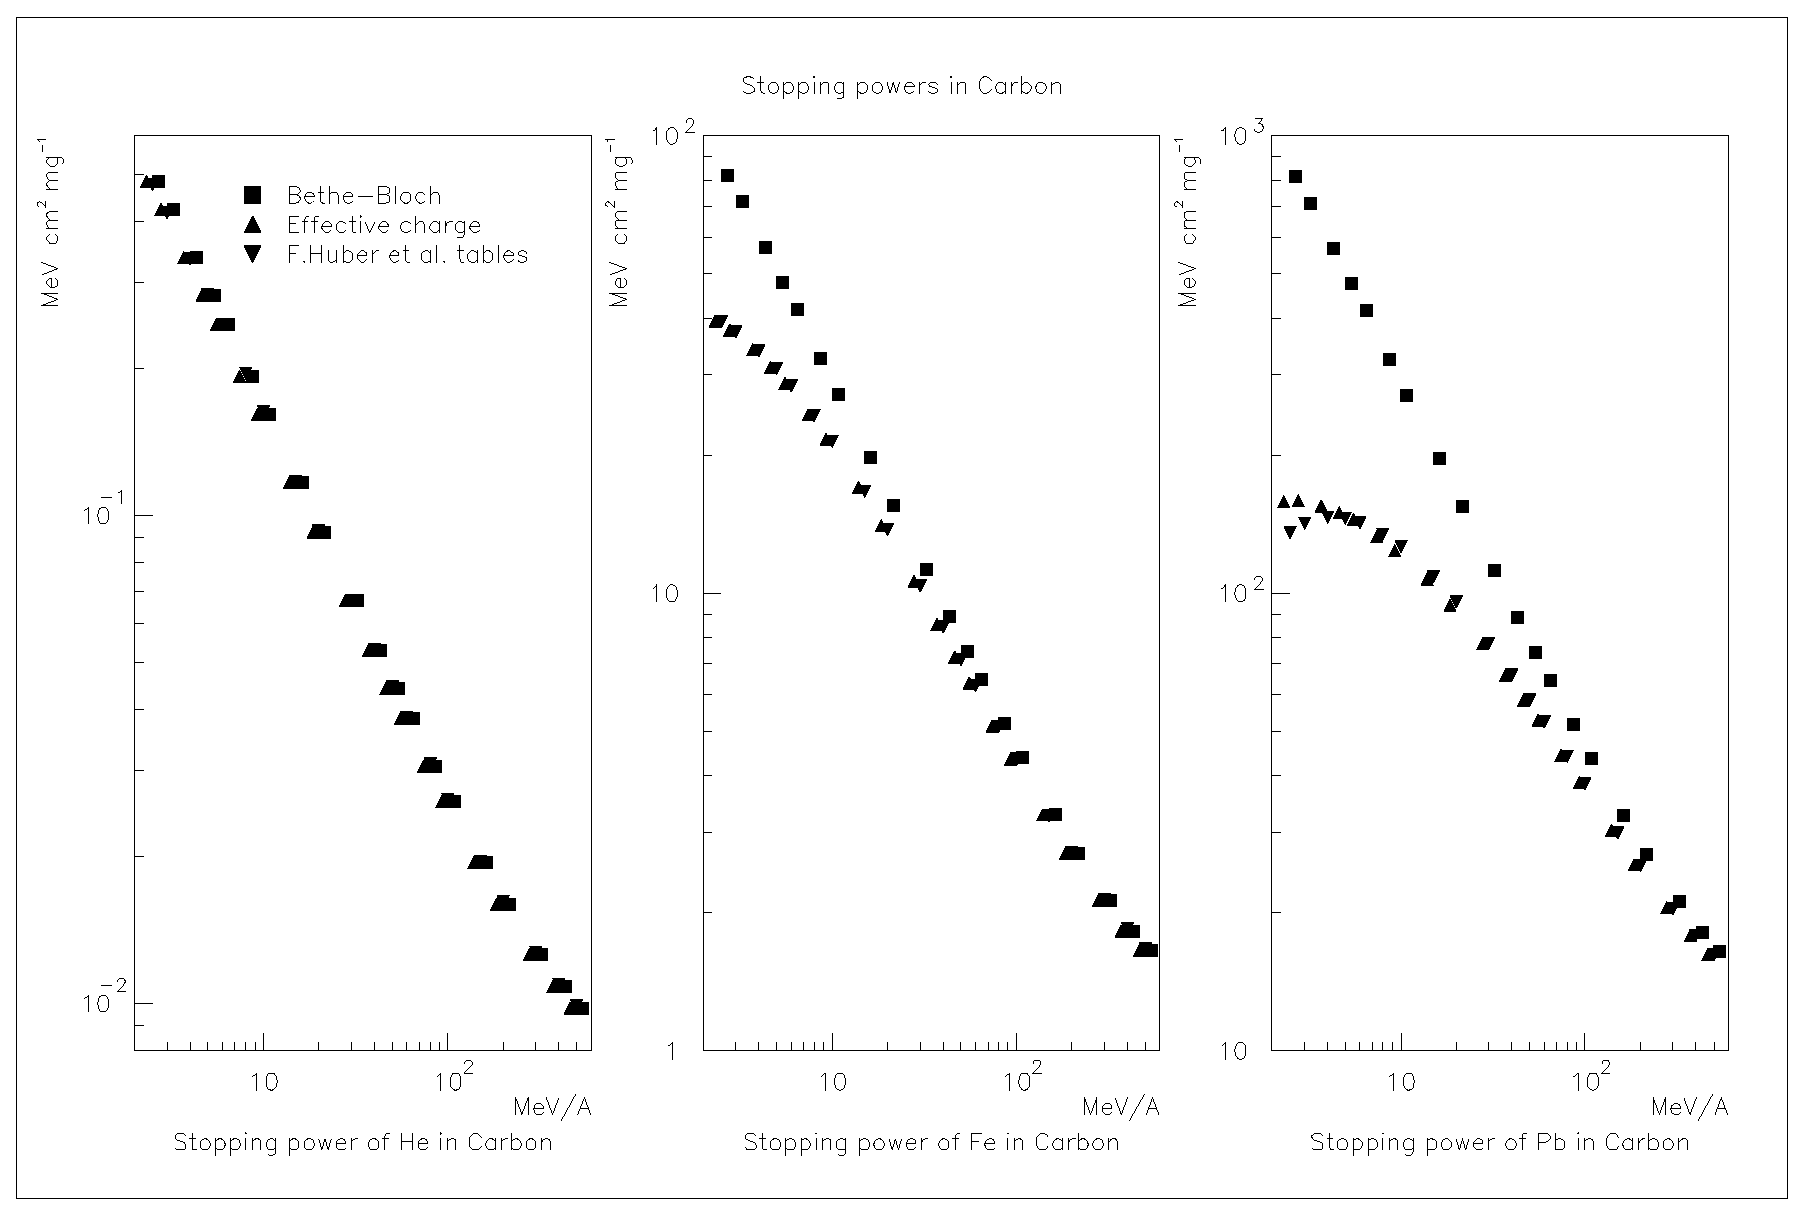
\epsfig{file=eps/phys431-1.eps,width=14cm}
     \caption{Stopping powers in Carbon}
     \label{fg:phys431-1}
\end{figure}

The heavy ions are in the {\it Gaussian regime} (see {\tt [PHYS332]})
of the collisional fluctuations even in the case of very thin absorbers.
If $T/A$ is not too high, the $\sigma^{2}$ of the distribution:
\begin{equation}
\label{eq:phys431-3}
\sigma^{2}_{coll} = D \frac{Q_{eff}^{2} Z}{A} \rho \; t \; m
\left [ 1 + \frac{T_{A}}{M_{u}} + \frac{1}{2} \left ( \frac{T_{A}}{M_{u}}
\right ) ^{2} \right ]
\end{equation}
where
\begin{DLtt}{MMMMMMMM}
\item[$D$] $\displaystyle 0.307 \frac{\mbox{MeV cm$^{2}$}}{\mbox{g}}$;
\item[$T_{A}$] $\displaystyle \frac{T}{A}$;
\item[$M_{u}$] atomic mass unit;
\item[$Z$] atomic number of the medium;
\item[$A$] mass number of the medium.
\end{DLtt}

\begin{table}
\begin{centering}
\begin{tabular}{|r|rr|r|rr|r|rr|r|}
\hline
& \multicolumn{9}{c|}{Pb ions in gas (energies in MeV)} \\
& \multicolumn{3}{c|}{N$_{2}$} & 
\multicolumn{3}{c|}{Ar} & 
\multicolumn{3}{c|}{Xe} \\
& \multicolumn{2}{c}{MonteCarlo} & \multicolumn{1}{c|}{data} &
\multicolumn{2}{c}{MonteCarlo} & \multicolumn{1}{c|}{data} &
\multicolumn{2}{c}{MonteCarlo} & \multicolumn{1}{c|}{data} \\
t (cm) & 
$\Delta$E & FWHM & FWHM & $\Delta$E & FWHM & FWHM & $\Delta$E & FWHM & FWHM \\
\hline
0.2 & 25.9 & 1.15 & 1.1 & 25.4 & 1.30 & 1.4 & 51.1 & 2.26 & 2.5 \\
0.4 & 53.6 & 1.62 & 1.5 & 52.4 & 1.84 & 1.9 & 107.0 & 3.22 & 3.3 \\
0.8 & 112.0 & 2.25 & 2.0 & 111.0 & 2.59 & 2.6 & 236.0 & 4.51 &  \\
1.2 & 162.0 & 2.37 & 2.0 & 168.0 & 2.95 & 2.8 & & & \\
\hline
\end{tabular}
\caption{Comparison of the measured and calculated and FWHM
for 1.4 MeV/A Pb ions in gas.}
\end{centering}
\label{tb:phys431-3}
\end{table}

Analysing the experimental straggling data it is possible to find that
the electron-exchange charge fluctuations can be described by a Gaussian
with width:
\begin{equation}
\label{eq:phys431-4}
\sigma^{2}_{ch} = D \frac{Q_{eff}^{2} Z}{A} \rho \; t \; m \frac{C}{2}
\left ( 1 - \frac{Q_{eff}}{Z_{I}} \right )
\end{equation}
where the parameter $C \sim 2.5$ has been derived
from the experimental straggling data.

If $Q_{eff} \rightarrow Z_{I}$, which is the case for high energy
heavy ions and for few MeV/A He ions, then $\sigma^{2}_{ch} \rightarrow 0$.


Comparing equations (\ref{eq:phys431-3}) and (\ref{eq:phys431-4}) it can be 
seen that for heavy ions and for $T/A \ll M_{u}$ $\sigma^{2}_{ch}
> \sigma^{2}_{coll}$. The total energy loss fluctuation can be
described by a Gaussian distribution with:
\begin{equation}
\sigma^{2} = \sigma^{2}_{ch} + \sigma^{2}_{coll}
\end{equation}

The mean energy loss and energy loss fluctuation calculation is performed
in the routine \Rind{GTHION}, making use of the proton energy loss tables.

{\bf Note:} The Gaussian fluctuation gives too broad a distribution for
high energy in the case of thin absorbers. A correction has been introduced
in \Rind{GTHION} which cures this discrepancy. In the absence of high
energy straggling data for ions, the correction has been tuned using 
high energy $\pi$ energy loss data, where the $\pi$ has been tracked
by \Rind{GTHION}.

\section{Comparison with data}

\subsection{Mean energy loss and range}

A test has been made against the distributions reported in~\cite{bib-HEIN}
for He ions at 1 and 10 MeV/A and for O and Pb ions at 1, 10 and
100 MeV/A in carbon and the results were found
to be correct within $5\%$ both for the energy loss and the range.

\begin{figure}[hbt]
     \centering
     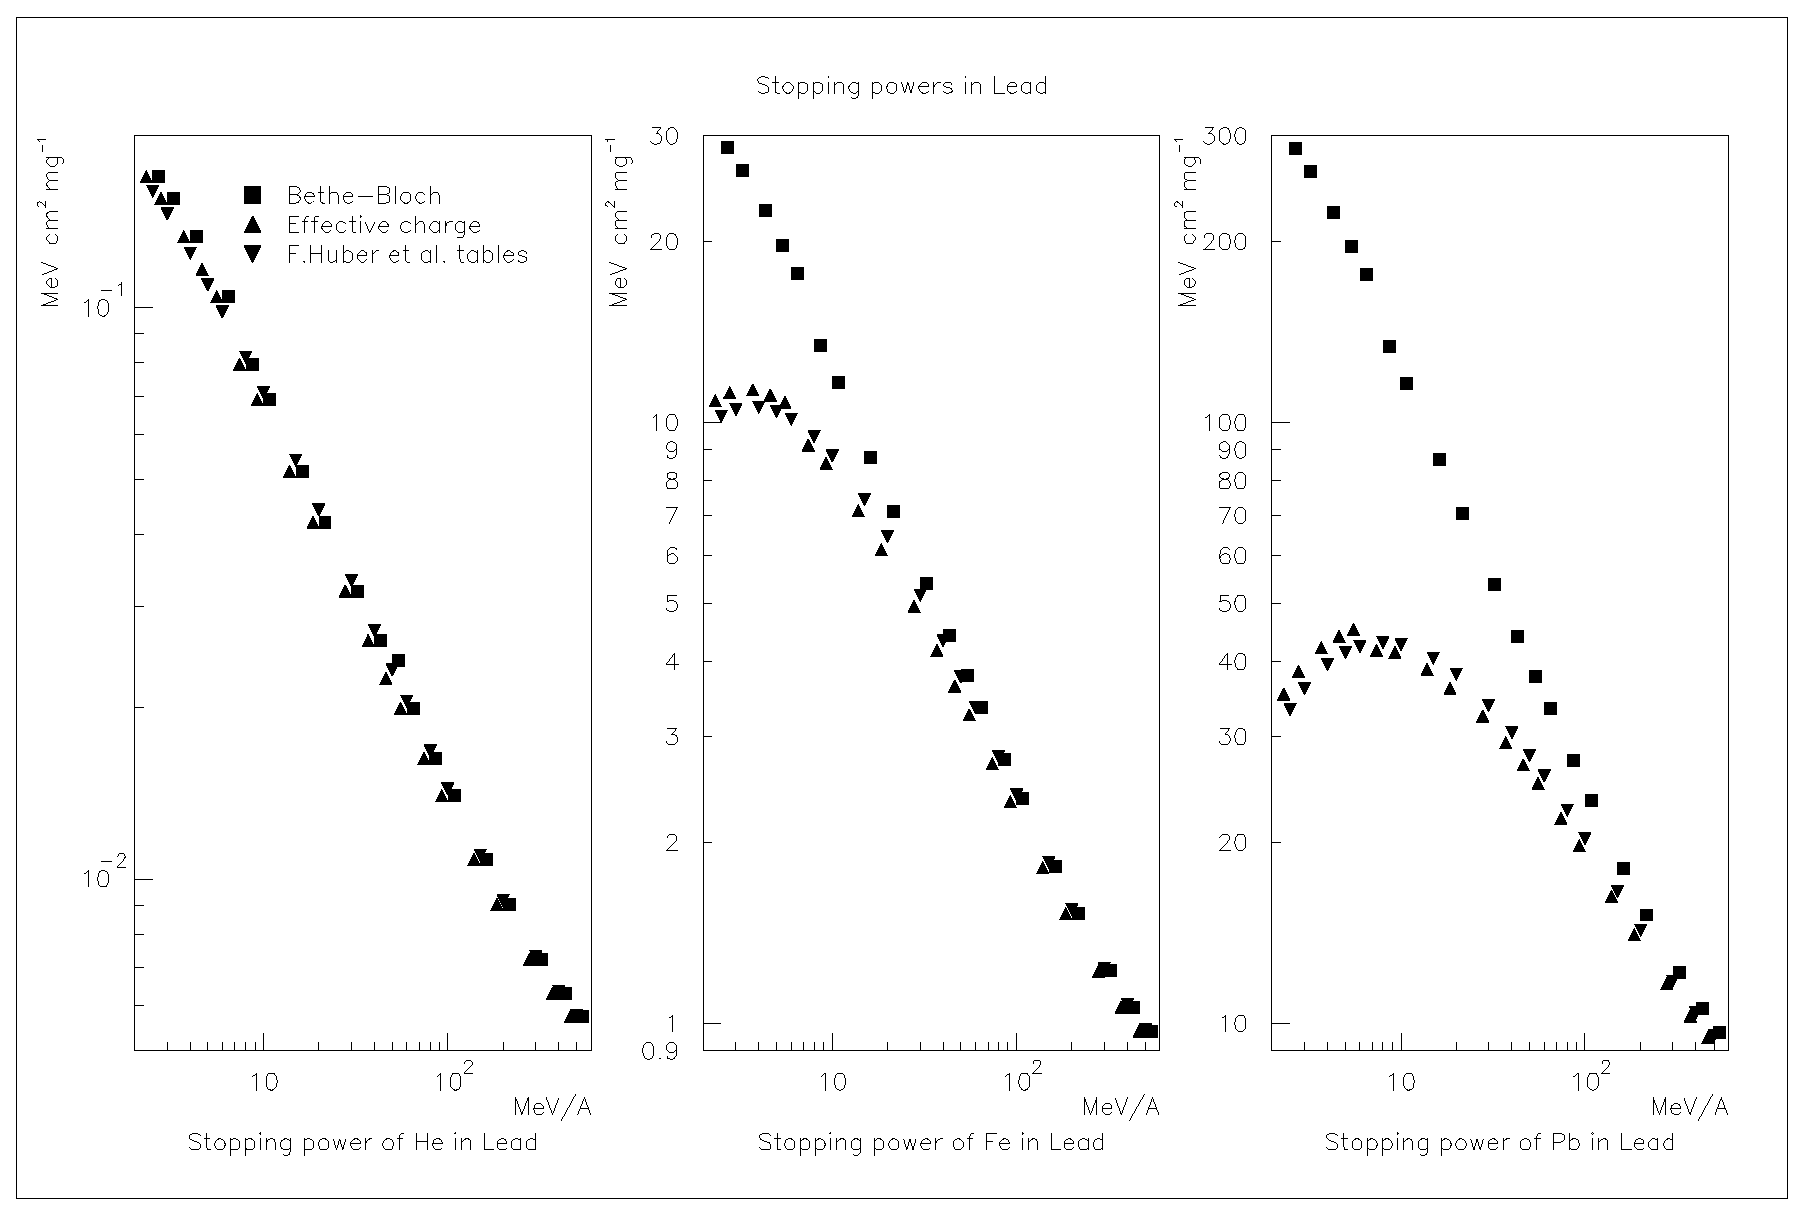
\epsfig{file=eps/phys431-2.eps,width=14cm}
     \caption{Stopping powers in Lead}
     \label{fg:phys431-2}
\end{figure}

Another comparison has been made with the tables of~\cite{bib-HUBE} 
for 10 MeV/A ions in lead, with
the results shown in table~\ref{tb:phys431-1}.
Another comparison with the same tables is shown in Figs.~\ref{fg:phys431-1}
and \ref{fg:phys431-2}.

A comparison with the tables in~\cite{bib-ANZI,bib-ANZ1} for T/A $<$ 1 MeV/A
gives  an error on $(dE/dx) \leq 10-20\%$.

\begin{table}
\begin{centering}
\begin{tabular}{|r|rr|r|}
\hline
\multicolumn{4}{|c|}{He ions in Ar (energies in keV)} \\
& \multicolumn{2}{c}{MonteCarlo} & \multicolumn{1}{c|}{data} \\
t (cm) & 
$\Delta$E & FWHM & FWHM \\
\hline
0.5 & 444 & 38 & $\sim$40 \\
1.0 & 913 & 53 & $\sim$60 \\
2.0 & 1940 & 78 & $\sim$80 \\
\hline
\end{tabular}
\caption{Comparison of the measured and calculated and FWHM
for 1.4 MeV/A He ions in gas.}
\end{centering}
\label{tb:phys431-4}
\end{table}

\subsection{Comparison of FWHM}

A comparison has been made with 
low energy data ($0.3 \leq T/A \leq 2.5$ MeV/A) in very
thin absorbers (1,7 $\mu$m, 0.4 $\mu$m). Data are taken from
the tables in~\cite{bib-TSCH} for
energy loss of O ions in Al, and the
results are reported in table~\ref{tb:phys431-2}. The quoted experimental 
error for these data is $1\%$ statistical + $5\%$ systematic for 
417 $\mu$g cm$^{-2}$ data and $2\%$ statistical + $10\%$ systematic for
110 $\mu$g cm$^{-2}$ data. 

Plots of energy deposition distributions of 1.4 MeV/A lead and helium
ions in gases can be found in~\cite{bib-GEIS}. 
From these we have measured the FWHM and compared them with the ones given
by the MonteCarlo. The results can be seen in table~\ref{tb:phys431-3}
and ~\ref{tb:phys431-4}. It
should be noted that the absorber thickness of, for example, Ar compares
with that of the preceding case (0.2 cm Ar = 356 $\mu$g cm$^{-2}$ and
1.2 cm Ar = 2136 $\mu$g cm$^{-2}$).


Similar comparison has been made for C ions of energies 17.1 and 39.4 MeV in 
isobuthane~\cite{bib-SCHM} and the agreement between data and {\tt GEANT}
for FWHM is within 30\%.

%%%%%%%%%%%%%%%%%%%%%%%%%%%%%%%%%%%%%%%%%%%%%%%%%%%%%%%%%%%%%%%%%%%
%                                                                 %
%  GEANT manual in LaTeX form                              %
%                                                                 %
%  Michel Goossens (for translation into LaTeX)                   %
%  Version 1.00                                                   %
%  Last Mod. Jan 24 1991  1300   MG + IB                          %
%                                                                 %
%%%%%%%%%%%%%%%%%%%%%%%%%%%%%%%%%%%%%%%%%%%%%%%%%%%%%%%%%%%%%%%%%%%
\Origin{L.Urb\'{a}n}
\Version{Geant 3.16}\Routid{PHYS440}
\Submitted{26.10.84}  \Revised{16.12.93}
\Makehead{Total cross-section and energy loss for bremsstrahlung by
Muons}
\section{Subroutines}
\Shubr{GBRELA}{}
{\tt GBRELA} fills the tables for continuous energy loss of electrons,
positrons and muons due to bremsstrahlung during initialisation time.
The energy binning is determined by
the array {\tt ELOW} (common \FCind{/CGMULO/}) in the
routine \Rind{GPHYSI}. In the tables, the $dE/dx$ due to bremsstrahlung
is summed with that due to the ionisation. For energy loss
of muons, \Rind{GBRELA} calls the function \Rind{GDRELM}.
The following pointers are used:
\begin{DLtt}{MMMMMMMMMMMMMMMMMM}
\item[JMA = LQ(JMATE-I)] pointer to the I$^{th}$ material;
\item[JEL1 = LQ(JMA-1)]  pointer to dE/dx for electrons;
\item[JEL1+NEK1]           pointer to dE/dx for positrons;
\item[JEL2 = LQ(JMA-2)]  pointer to dE/dx for electrons.
\end{DLtt}
\Rind{GBRELA} is called by \Rind{GPHYSI}.
\Sfunc{GBRELM}{VALUE = GBRELM(Z,T,BCUT)}
\begin{DLtt}{MMMMMMMM}
\item[Z] ({\tt REAL}) atomic number of the material;
\item[T] ({\tt REAL}) kinetic energy of the muon;
\item[BCUT] ({\tt REAL}) {\it soft} bremsstrahlung cut.
\end{DLtt}
\Rind{GBRELM} calculates the muon energy loss due to bremsstrahlung
of photons with energy below {\tt BCUT}, (variable {\tt BCUTM} in the
common \FCind{/GCCUTS/}).
Above this value, the bremsstrahlung process is simulated
explicitly (see {\tt [PHYS441]}) and the energy lost by the muons is
not included in the tables. 
In the tables, the $dE/dx$ due to bremsstrahlung is summed with
the energy lost coming from ionisation, pair production and nuclear interaction.
\Rind{GBRELM} is called by \Rind{GBRELA}.
\Shubr{GBRSGA}{}
{\tt  GBRSGA} calculates the total cross-section for bremsstrahlung.
It tabulates the mean free path
in cm as a function of the medium and the energy. The energy
binning is determined by the array {\tt ELOW} (common \FCind{/CGMULO/}).
The following pointers are used:
\begin{DLtt}{MMMMMMMMMMMMMMMMMM}
\item[JMA = LQ(JMATE-I)]pointer to the I$^{th}$ material;
\item[JBREM = LQ(JMA-9)]pointer to bremsstrahlung cross-sections;
\item[JBREM            ]pointer for \Pem;
\item[JBREM+NEK1       ]pointer for \Pep;
\item[JBREM+2*NEK1     ]pointer for $\mu^+/\mu^-$.
\end{DLtt}
\Rind{GBRSGA} is called during initialisation by \Rind{GPHYSI}.
\Sfunc{GBRSGM}{VALUE = GBRSGM(Z,T,BCUT)}
\begin{DLtt}{MMMMMMMM}
\item[Z] ({\tt REAL}) atomic number of the materian;
\item[T] ({\tt REAL}) kinetic energy of the muon;
\item[BCUT] ({\tt REAL}) {\it soft} bremsstrahlung cut.
\end{DLtt}
\Rind{GBRSGM} calculates the total bremsstrahlung cross-section for
muons when the emitted photon has an energy greater than {\tt BCUT}, 
(variable {\tt BCUTM} in the common \FCind{/GCCUTS/}). It is called
by \Rind{GBRSGA}.
\section{Method}
 
The mean value of the energy lost by the muon due to bremsstrahlung of
photons of energy $<k_{c}$ = {\tt BCUTM} is:
\begin{equation}
\label{eq:phys440-1}
E_{loss}^{brem}(Z,T,k_c ) = \int_{0}^{k_c} k
        \frac{d \sigma (Z,T,k)}{dk}dk
\end{equation}
and the total cross-section for the emission of a photon of energy
$ > k_c $ is
\begin {equation}
\label{eq:phys440-2}
 \sigma (Z,T,k_c ) = \int_{k_c}^{T}
        \frac{d \sigma (Z,T,k)} {dk} dk
\end{equation}
Accurate cross-section formula for the high energy ($T \geq 1$ GeV)
muon bremsstrahlung can be found in \cite{bib-LOHM}.

\subsection{Parameterisation of energy loss and total cross-section}
The cross-sections from \cite{bib-LOHM} have been used to calculate 
{\it data} points for (\ref{eq:phys440-1}) and (\ref{eq:phys440-2}).
These have been parameterised as:
\[ \begin{array}{LcLl}
 \sigma (Z,T,k_c)& =& Z[Z+ \xi_{\sigma}(1+ \gamma \ln Z)]
       \left[\ln \frac{k_{max}}{k_c}\right]^{\alpha}
       F_{\sigma}(Z,X,Y) & \mbox{ in barn} \\
  E_{loss}^{brem} (Z,T,k_c)   & = & Z[Z+\xi_l(1+\delta\ln Z)]
   \left[\ln\frac {k_c} {E} \right]^{\beta}
    F_l(Z,X,Y) & \mbox{ in GeV barn}
\end{array} \]
\[ \begin{array}{LcL@{\hspace{2cm}}LcL}
k_{max} & = & E-0.75 \sqrt {e}m_{\mu}Z^{1/3} & X & = & \ln \frac{E}{m_{\mu}} \\
Y & = & \ln \frac{k_c}{m_{\mu}} & E & = & T+m_{\mu}
\end{array} \]
where  $k_{max}$ is the maximum
possible value of the photon energy.
The functions $F_i(Z,X,Y)$ ($i=\sigma ,l$) are polynomials:
\begin{eqnarray}
\label{eq:phys440-3}
F_i(Z,X,Y) & = & (C_1+C_2X+\cdots +C_6X^5)+(C_7+C_8X+\cdots+C_{12}X^5)Y
\nonumber \\
        & + & \cdots + (C_{31}+C_{32}X+\cdots+C_{36}X^5)Y^5
\nonumber \\
           & + & Z[(C_{37}+C_{38}X+\cdots+C_{40}X^3)+(C_{41}+C_{42}X+
                   \cdots+C_{44}X^3)Y \nonumber \\
           & + & \cdots + (C_{48}+C_{49}X+\cdots+C_{52}X^3)Y^3)]
\end{eqnarray}
A least-squares fit has been performed on more than 2000 points for
$Z = 1, 6, 13, 26, 50, 82, 92$ and 1 GeV $\leq T \leq $ 10 TeV and
10 keV $\leq k_c \leq T $. The resulting values of 
$\xi_{\sigma,l}$, $\gamma$, $\alpha$ ,$C_i$, $\xi_l$, $\delta$ and $\beta$
can be found in the {\tt DATA} statements within the functions
\Rind{GBRSGM} and \Rind{GBRELM} which
compute formulae (\ref{eq:phys440-1}) and (\ref{eq:phys440-2}) respectively.
 
The accuracy of the fit can be estimated as:\\
 
\[ \begin{array}{LcL}
\frac{\Delta \sigma}{\sigma} & = & \left \{
\begin{array}{p{2cm}lL}
$\displaystyle 10-12\%$ & \mbox{if} & T \leq 5 \: \mbox{GeV} \\
$\displaystyle \leq 4\%$ & \mbox{if} & T > 5 \: \mbox{GeV}
\end{array} \right . \\ [0.5cm]
\frac{\Delta E_{loss}^{brem}}{E_{loss}^{brem}} & = & \left \{
\begin{array}{p{2cm}lL}
$\displaystyle 10\%$ & \mbox{if} & T \leq 5 \: \mbox{GeV} \\
$\displaystyle \leq 3\%$ & \mbox{if} & T > 5 \: \mbox{GeV}
\end{array} \right .
\end{array} \]
 
The contribution of the bremsstrahlung to the total energy loss of
the muons is less than 1\% for $ T \leq$ 5 GeV.
 
When $k_{c} \geq k_{max}$, a parameterisation different from 
(\ref{eq:phys440-3}) can be used for the total muon energy loss due to 
bremsstrahlung:
\begin{eqnarray} 
\label{eq:phys440-4}
E_{loss}^{brem} (Z,T) & = & E_{loss}^{brem}(Z,T,k=k_{max}) 
\nonumber\\
& = & Z(Z+1) k_{max}[d_1+(d_2X+d_3Y) + (d_4X^2+d_5 XY+d_6 Y^2) \nonumber \\
& + & \cdots+(d_{22}X^6+d_{23}X^5 Y+\cdots+d_{28}Y^6)]
\end{eqnarray}
where $Y=Z^{1/3}$. 
The accuracy of the formula (\ref{eq:phys440-4}) for $1 \leq Z \leq 100$
is rather good:
\[
\frac{\Delta E_{loss}^{brem}}{E_{loss}^{brem}} = \left \{
\begin{array}{LlL}
\leq 1.5\% & \mbox{if} & T > 1  \; \mbox{GeV} \\
\leq 1\%  & \mbox{if} & T > 5 \; \mbox{GeV}
\end{array} \right .
\]

%%%%%%%%%%%%%%%%%%%%%%%%%%%%%%%%%%%%%%%%%%%%%%%%%%%%%%%%%%%%%%%%%%%
%                                                                 %
%  GEANT manual in LaTeX form                              %
%                                                                 %
%  Michel Goossens (for translation into LaTeX)                   %
%  Version 1.00                                                   %
%  Last Mod. Jan 24 1991  1300   MG + IB                          %
%                                                                 %
%%%%%%%%%%%%%%%%%%%%%%%%%%%%%%%%%%%%%%%%%%%%%%%%%%%%%%%%%%%%%%%%%%%
\Origin{L.Urb\'{a}n}
\Version{Geant 3.16}\Routid{PHYS441}
\Submitted {26.10. 84}   \Revised {11.10.93}
\Makehead{Simulation of discrete bremsstrahlung by muons}
\section{Subroutines}
\Shubr{GBREMM}{}
\Rind{GBREMM} generates a photon from bremsstrahlung of a highly 
energetic muon as a discrete process. For the 
angular distribution of the photon, is calls the function \Rind{GBTETH}.

\begin{DLtt}{MMMMMMMM}
\item[Input:] via common \Rind{/GCTRAK/};
\item[Output:] via common \Rind{/GCKING/}.
\end{DLtt}
 
\Rind{GBREMM} is called from the tracking routine 
\Rind{GTMUON} when the muon reaches its radiation 
point during the tracking stage of {\tt GEANT}.

\Sfunc{GBTETH}{VALUE = GBTETH(ENER,PARTM,EFRAC)}

\begin{DLtt}{MMMMMMMM}
\item[ENER] ({\tt REAL}) kinetic energy of the muon;
\item[PARTM] ({\tt REAL}) mass of the radiating particle ($m_{\mu}$ in
this case);
\item[EFRAC] ({\tt REAL}) ratio of the energy of the radiated photon
to the energy of the muon.
\end{DLtt}

\Rind{GBTETH} calculates the angular distribution of the \Pem\Pep pair
in photon pair production and of the photon in bremsstrahlung.
In case of bremsstrahlung it gives the scaled angle ($\eta = E\theta
m^{-1}$) of the photon.

\section{Method}
 
The differential cross-section for the emission of a photon of energy $k$ by
a muon of energy $E$ is \cite{bib-LOHM,bib-MARM}:
 
\begin{equation}
 \frac{d \sigma} {dv}= \frac{N} {v} \left (
 \frac{4} {3} -\frac{4} {3}  v+v^2  \right )  \Phi ( \delta )
\end{equation}
where
\begin{eqnarray*}
& & \begin{array}{LcL@{\hspace{1cm}}LcL}
N & = & \mbox{normalisation factor} & v  & = & \frac{k}{E}   \\
\delta   & = & \frac {m_{\mu}^2}{2E}\frac{v} {1-v} & e & = & 2.718\dots 
\end{array} \\ [0.2cm]
\Phi(\delta)  & = & \left \{
\begin{array}{LlL}
\ln\left(\frac{189 m_{\mu}}{m_{e} Z^{1/3}}\right)
        -\ln\left(\frac{189\sqrt{e}} {m_{e} Z^{1/3}}\delta +1\right)
                   & \mbox{if}& Z \leq 10    \\ [0.4cm]
\ln\left(\frac{189 m_{\mu}}{m_{e} Z^{1/3}}\right)
        -\ln\left(\frac{189\sqrt{e}} {m_{e} Z^{1/3}}\delta +1\right)
+\ln \left(\frac{2}{3}Z^{-1/3} \right)
                   & \mbox{if}& Z > 10 
\end{array} \right . \\ [0.2cm]
v_c          & = & \frac{k_c}{E}\leq v \leq
                   \left( 1- 0.75\sqrt{e}\frac{m_{\mu}}{E}Z^{1/3} \right)
                   = v_{max}
\end{eqnarray*}
Therefore, the differential cross-section can be written as
\begin{equation}
 \frac{d \sigma} {dv} = f(v) g(v)
\end{equation}
with
\begin{eqnarray*}
f(v) & = & \left[v \ln \left( \frac{v_{max}}{v_c}\right)\right]^{-1} \\
g(v) & = & \frac{1}{\Phi(0)} \left(1-v +\frac{3}{4}v^2\right)\Phi(\delta)
\end{eqnarray*}
We can sample the photon energy in the following way
($r_1$, $r_2$ uniformly distributed random numbers in $]0,1[$):
 
\begin{enumerate}
\item sample $v$:
\[
v= v_c \left(\frac{v_{max}}{v_c}\right)^{r_1}
\]

\item compute the rejection function $g(v)$ and:
\begin{enumerate}
\item if $ r_2 > g(v)$ go back to step 1
\item if $ r_2 \leq g(v)$, accept $v$ and $k = v E$.
\end{enumerate}
\end{enumerate}

After the successful sampling of $k$, \Rind{GBREMM} generates the polar
angles of the radiated photon with respect to an axis defined along the parent
muon's momentum calling \Rind{GBTETH}. For more information on the sampling
procedure see {\tt [PHYS341]}.

\include{phys450}
%%%%%%%%%%%%%%%%%%%%%%%%%%%%%%%%%%%%%%%%%%%%%%%%%%%%%%%%%%%%%%%%%%%
%                                                                 %
%  GEANT manual in LaTeX form                                     %
%                                                                 %
%  Version 1.00                                                   %
%                                                                 %
%  Last Mod. 12 June 1993 1800  MG                                %
%                                                                 %
%%%%%%%%%%%%%%%%%%%%%%%%%%%%%%%%%%%%%%%%%%%%%%%%%%%%%%%%%%%%%%%%%%%
\Origin{L.Urb\'{a}n}
\Version{Geant 3.10}\Routid{PHYS451}
\Submitted{26.10.84}   \Revised{16.12.93}
\Makehead{Simulation of  e+e- pair  production by  muons}
\section{Subroutines}
\Shubr{GPAIRM}{}
\Rind{GPAIRM} generates the \Pep\Pem-pair radiated by a high energetic muon.
It uses the following input and output:
\begin{DLtt}{MMMMMMM}
\item[input:]  via common block \FCind{/GCTRAK/}
\item[output:] via common block \FCind{/GCKING/}
\end{DLtt}
\Rind{GPAIRM} is called automatically from the tracking routine
\Rind{GTMUON} if, and when,
the parent muon reaches its radiation point during the tracking.
\section{Method }
The double differential cross-section for the
process can be written \cite{bib-LOHM}:
 \begin{eqnarray}
\frac {d^2 \sigma}{d\nu d \rho}&=& \alpha^4\frac
     {2} {3 \pi} (Z \lambda)^2 \cdot  \frac {1-\nu}{\nu}\left [\phi_{\rm e} +
     (m/M)^2
     \phi_{\mu} \right ]
\end{eqnarray}
All the quantities in the expression above are defined in {\tt [PHYS450]}.
 By computing this cross-section for different
($\nu,\rho$) points, it can be seen that:
\begin{enumerate}
\item
the {\bf shape} of the functions
$\frac{\Tstm d^2 \sigma}{\Tstm d\nu d\rho}$
and
$\frac{\Tstm d \sigma}{\Tstm d\nu}\int d \rho \frac {\Tstm d^2 \sigma}
{\Tstm d\nu d\rho}$
practically does not depend on $Z$
\item
the dominant contribution comes from {\bf the low $\nu$ region:}
\begin{equation}
 \nu_{\rm min} = (4m/E)  \leq \nu  \leq  100*\nu_{\rm min}
\end{equation}
\item
in this low region ($d^2\sigma/d\nu d\rho$)
{\bf is flat} as a function of $\rho$
\end{enumerate}
Therefore, we propose the following sampling method as a rough approximation:
\begin{enumerate}
\item
In the low $\nu$ region the differential cross-section
\[
\frac{d \sigma}{d\nu}=\int d \rho \frac{d^2 \sigma K} {d\nu d\sigma}
\]
can be approximated as:
\begin{equation}
\frac{d \sigma}{d\nu} \approx  \left[1-\frac{\nu_{\rm min}}{\nu}\right]^{1/2}
      \frac{1}{v^a} \mbox{\qquad with:\quad}
a = 2-\frac{\ln E}{10} \mbox{\qquad($E$ in GeV)}
\end{equation}
We can write:
\begin{equation}
 \frac{d \sigma}{d\nu}\approx f(\nu) g(\nu)
\end{equation}
where,
\begin{equation}
f(\nu) = \frac{(a-1)}{\frac{\Tstm 1}{\Tstm \nu_c^{a- 1}}  -
        \left(\frac{\Tstm 1}{\Tstm \nu_{\rm max}}\right)^{a-1}}
        \frac{1}{\nu^a}
\end{equation}
is the normalised distribution in the interval $[\nu_c,\nu_{\rm max}]$ and
\begin{equation}
g(\nu) = \left[1-\frac{\nu_{\rm min}}{\nu}\right]^{1/2}
\end{equation}
is the rejection function.
\item
$r_1$ and $r_2$ being two uniformly distributed random numbers in the
interval $[0,1]$:
\begin{eqnarray}
& - & \mbox{Sample $\nu$ from the distribution $f(\nu)$ as:}\nonumber      \\
&   & \nu = \left(\frac{1-r_1}{\nu_c^{a-1}} \frac{r_1}{\nu_{\rm max}^{a-1}}
      \right)^\frac{\Sstm 1}{\Sstm 1-a}                                    \\
& - & \mbox{Accept $\nu$ if $r_2 \leq g(\nu)$}
\end{eqnarray}
\item Then compute
\begin{equation}
\rho_{\rm max}(\nu) = \left[1 -\frac{6M^2}
      {E^2(1-\nu)}\right]\left[1-\frac{4m}{\nu E}\right]^{1/2} \\
\end{equation}
and generate $\rho $ uniformly in the range $[-\rho_{\rm max},
+\rho_{\rm max}]$.
\end{enumerate}
After the successful sampling of ($ \nu,\rho $), \Rind{GPAIRM} generates the
polar
angles of the radiated \Pep\Pem-pair with respect to
an axis defined along the parent
muon's momentum. $\Theta$ is assigned the approximate average value:
\begin{equation}
 \Theta =\frac{M}{E}
\end{equation}
$\phi^+$ is generated isotropically and $\phi^- = \phi^+ + \pi$

%%%%%%%%%%%%%%%%%%%%%%%%%%%%%%%%%%%%%%%%%%%%%%%%%%%%%%%%%%%%%%%%%%%
%                                                                 %
%  GEANT manual in LaTeX form                              %
%                                                                 %
%  Michel Goossens (for translation into LaTeX)                   %
%  Version 1.00                                                   %
%  Last Mod. Jan 24 1991  1300   MG + IB                          %
%                                                                 %
%%%%%%%%%%%%%%%%%%%%%%%%%%%%%%%%%%%%%%%%%%%%%%%%%%%%%%%%%%%%%%%%%%%
\Origin{H.C.Fesefeldt, F.Carminati}
\Documentation{F. Carminati}
\Version{Geant 3.10}\Routid{PHYS460}
\Submitted{20.12. 85}     \Revised{16.12.93}
\Makehead{Muon-nucleus interactions}
\section{Subroutines}
\Shubr{GMUNUI}{}
\Rind{GMUNUI} computes and stores in the appropriate bank the value of
the muon-nucleus cross-section for a given material.
It is called at initialisation time by \Rind{GPHYSI}.
\Shubr{GMUNU}{}
\Rind{GMUNU} is called by \Rind{GTMUON} every time a muon-nucleus interaction
has to happen. It generates the final state particles as well as the outgoing
muon. A call to \Rind{GUHADR} is performed if {\tt IMUNU} (which is the
variable set by the {\tt  MUNU} data record) is equal to 1. 
An inelastic interaction is forced (which could also be a fission in case 
of heavy materials).
The secondaries from the $\pi$-nucleus interaction are always generated
if {\tt IMUNU}
is equal to 1, irrespectively of the value of {\tt IHADR}.

{\bf Note:} {\tt IMUNU} should be set to 1 only when using the {\tt GHEISHA}
hadronic interactions package. Setting it to 1 when using {\tt FLUKA} can
give unpredictable results.

\Sfunc{GMUSIG}{VALUE = GMUSIG(E,E1,COSTET)}
\begin{DLtt}{MMMMMMMM}
\item[E] ({\tt REAL}) initial $\mu$ energy;
\item[E1] ({\tt REAL}) final $\mu$ energy;
\item[COSTET] ({\tt REAL}) $\mu$ scattering angle.
\end{DLtt}
This function returns the value of the differential cross-section in
millibarns for a muon of energy {\tt E} to generate 
a nuclear interaction recoil with
energy {\tt E1} at an angle the cosine of which is
{\tt COSTET}.

\section{Method}
This set of routines generates the interactions of muons with the nuclei of
the tracking material. The code is a straight translation into the {\tt GEANT} 
style
of the corresponding code from the {\tt GHEISHA} Monte Carlo Program.
The {\tt GHEISHA} routines {\tt CASMU} and {\tt CALIM} have been used 
\cite{bib-GHEI}.
 
The information contained in this chapter is mainly taken from the {\tt GHEISHA}
manual to which the user is referred.
The muon-nucleus inelastic cross-section is taken as 0.0003 mb for
a nucleon when the energy of the incoming muon is $E<30$ GeV, and slowly
increases for $E>30$ GeV according to the law:
\begin{center}
\[
\sigma = 0.3 * (E/30)^{0.25}\quad [\mu \rm b]
\]
\end{center}
The energy and angle of final state muon is generated according to the ``free
quark parton model''. If $E$ is the energy of the incoming muon and
$\Omega$ and $W$ the
angle and the energy of the outgoing muon, the differential cross-section
can be written as:
 
\[
\frac{d \sigma}{d \Omega dW} =\gamma ( \sigma_T + \epsilon \sigma_S)
\]
where:
\begin{eqnarray*}
\Gamma   & = & \frac{k \alpha}{2 \pi}\frac{W}{E}\frac{1}{1- \epsilon } \\
\epsilon & = & \left [ 1+2 \frac{Q^2 + \nu^2}{Q^2}\tan^2 \theta^2 \right]
\end{eqnarray*}
 
$Q^2$ and $\nu$ are the normal scaling variables expressed by:
 
\[
Q^2 = -q^2 = 2(EW-|p||p'|\cos\theta-m^2_{-\mu})\mbox{\quad and\quad} \nu
= E-W 
\]
 here $\sigma_T$ and $\sigma_S$ are the photo-absorption
cross-sections for transverse and
longitudinal photons respectively for which the relation used is:
 
\[
\sigma_S = 0.3 \left ( 1- \frac{1}{1.868}{Q^2}{\nu}\right)  \sigma_T
\]
and $\sigma_T$ is assumed to be constant $\sigma_T = 0.12 $ mb.
For the incident flux $K$ of
the photons Gillman's convention is used:
\[
K = \nu + Q^2/2\nu
\]
 A three-dimensional importance sampling in the variables $E$, $W$ and
$\theta$ is performed each time an interaction has to occur.
 
This set of routines only works if \Rind{GUPHAD} calls \Rind{GPGHEI} and
\Rind{GUHADR} calls \Rind{GHEISH}.
The hadrons are generated in an approximate way. The virtual photon is
replaced by a real pion of random charge with the same kinetic energy. Then the
\Rind{GUHADR} routine is called to generate a $\pi$-nucleus inelastic
scattering. While the final state generated this way gives a good
approximation for calorimetric purposes, the kinematics of the final state
may be a rather poor approximation of reality.
The muon-nucleus interactions are activated by the {\tt  MUNU} data record of
{\tt GEANT}. After a muon-nucleus interaction the muon will still be the current
particle. If {\tt MUNU} 1 has been specified, secondaries coming from the
interaction of the virtual photon with the nucleus will be in the {\tt GEANT}
temporary stack. If {\tt MUNU} 2 has been specified, then the secondary
particles will not be generated and the energy lost by the muon will be
added to {\tt DESTEP}.
For each material a table of muon-nucleus cross-sections is stored at
initialisation time. See material bank structure for details.

%%%%%%%%%%%%%%%%%%%%%%%%%%%%%%%%%%%%%%%%%%%%%%%%%%%%%%%%%%%%%%%%%%%
%                                                                 %
%  GEANT manual in LaTeX form                              %
%                                                                 %
%  Michel Goossens (for translation into LaTeX)                   %
%  Version 1.00                                                   %
%  Last Mod. Jan 24 1991  1300   MG + IB                          %
%                                                                 %
%%%%%%%%%%%%%%%%%%%%%%%%%%%%%%%%%%%%%%%%%%%%%%%%%%%%%%%%%%%%%%%%%%%
\Origin{H.C. Fesefeldt, F.Carminati}
\Documentation{F. Carminati}
\Version{Geant 3.16}\Routid{PHYS510}
\Submitted{24.02.86}       \Revised{11.10.93}
\Makehead{The GEANT/GHEISHA Interface}
\section{Introduction }
 
There are two packages to describe the hadronic showers in matter
which are available to the users of {\tt GEANT}: {\tt GHEISHA}~\cite{bib-GHEI}
and {\tt FLUKA} (see {\tt [PHYS520]}).
 
The {\tt GHEISHA} code generates hadronic interactions with the nuclei of the
current tracking medium, evaluating cross-sections and sampling the final 
state multiplicity and kinematics, while the {\tt GEANT} philosophy is 
preserved for the tracking.
The {\tt GHEISHA} code is stored in the {\tt GEANH} car file.

The {\tt GHEISHA} printing flags can be set via the {\tt GEANT} {\tt SWIT} 
data record:
each switch greater than 100 but smaller that 111 sets the
corresponding printing flag of {\tt GHEISHA} modulo 100, so that {\tt
SWIT 105} will set the printing flag 5 of {\tt GHEISHA}. Setting the
printing flags of {\tt GHEISHA} the following information will be displayed:
\begin{DLtt}{MMMMMMMM}
\item[NPRT(1)]    one header for each track in the shower;
\item[NPRT(2)]    all tracking information;
\item[NPRT(3)]    kinematic of decays (not effective);
\item[NPRT(4)]    kinematic of nuclear interactions;
\item[NPRT(5)]    kinematic of electromagnetic interactions (not effective);
\item[NPRT(6)]    material constants, dE/dX and absorbed energies
                  (not effective);
\item[NPRT(7)]    event summary;
\item[NPRT(8)]    history of all interactions/decays;
\item[NPRT(9)]    free;
\item[NPRT(10)]   tables of the geometry, cross-sections, etc.;
\end{DLtt}
{\tt NPRT(1), NPRT(2)} and {\tt NPRT(6)} should be used only in case  of
suspected errors. {\tt NPRT(8)} produces the most illustrative output. Those
flags work in conjunction with the {\tt DEBUG} data record 
of {\tt GEANT}.
\subsection{Description of the routines }
\Shubr{GHESIG}{(P,EK,AVER,A,Z,W,NLM,DENS,CORR,IPART)}
\begin{DLtt}{MMMMMMMMMM}
\item[P] ({\tt REAL}) momentum of the particle (in GeV/c);
\item[EK] ({\tt REAL}) kinetic energy of the particle (in GeV);
\item[AVER] ({\tt REAL}) average mass number of the material;
\item[A(NLM)] ({\tt REAL}) vector containing the mass numbers 
of the components of the mixture, the same as {\tt AVER} in case of an
element;
\item[Z(NLM)] ({\tt REAL}) vector containing the atomic numbers of the
components of the mixture, or the atomic number in case of an element;
\item[W(NLM)] ({\tt REAL}) vector of length NLM containing the relative weights
of  the  components of the mixture (normalised to one), one in case of an
element;
\item[NLM]  ({\tt INTEGER}) number of components of the mixture, $1$ in case 
of an element;
\item[DENS]  ({\tt REAL}) density of the material;
\item[CORR]  ({\tt REAL}) if this parameters is $>0$, then corrections are
applied to the cross-section; should be used in case of inorganic 
scintillators;
\item[IPART] ({\tt INTEGER}) {\tt GEANT} particle code.
\end{DLtt}
This routine returns the total macroscopic cross-section in cm$^{-1}$. 
The correction flag is taken from the $26^{th}$ word of the {\it next}
bank in the tracking medium linear structure pointed at by 
{\tt LQ(JTMED-NUMED)}.
 
The cross-sections on nucleus are known only for pions and protons. The
general law:
\[
\sigma(A) = 1.25*\sigma_{tot}^{Proton} \; A^\alpha
\]
is used but it is valid only for momenta $>$ 2 GeV. The parametrisation done
gives only a behaviour averaged over momenta and particle types. 
For H, Al, Cu and Pb the measured cross-sections are
stored in {\tt DATA} statements.
 
The stored cross-sections are the pre-calculated {\tt GHEISHA} ones.
As a starting point the measured cross-sections of pions, kaons,
protons, antiprotons and neutrons on protons are used. The cross-sections
tabulated are measured values taken from the CERN HERA compilations. The
values for K$^{0}_{s}$/K$^{0}_{l}$ are updated as of July 1980. 
Strange baryon cross-section
are calculated using a parametrisation in terms of quark-quark forward
scattering amplitudes and optical theorem. The additive quark quark scattering
model is used.
All the cross-sections are contained in data statements so no
external file is needed for {\tt GHEISHA}.
\Shubr{GPGHEI}{}
This routine returns the distance to the next hadronic interaction
according to the {\tt GHEISHA} cross-sections. It calls \Rind{GHESIG}
and is called by \Rind{GUPHAD}. The default copy provided in
the {\tt GEANT} library uses the {\tt GHEISHA} shower code:
\begin{verbatim}

       SUBROUTINE GUPHAD
* 
*****************************************************************
*                                                               *
*   GEANT  user routine called at each step to evaluate         *
*   the remaining distance to the hadronic interaction point    *
*                                                               *
*****************************************************************
*
      CALL GPGHEI
*
      END

      SUBROUTINE GUHADR
*.
****************************************************************
*                                                              *
*       GEANT  user routine called when a hadronic process     *
*       has been selected in the current step, in order to     *
*       generate the final particle's state                    *
*                                                              *
****************************************************************
* 
       CALL GHEISH
*
       END
\end{verbatim}

\Shubr{GHEISH}{}
This is the main steering routine for the hadronic interactions and is
a fan-out to the various {\it cascade} routines of
{\tt GHEISHA} which treat the particular hadronic interaction. Here the kind
of interaction is stored in the {\tt INT}
flag, with the following meaning:
\begin{DLtt}{MMMMMMMM}
\item[INT=0] no interaction            ({\tt NONE});
\item[INT=1] elastic scattering occurs ({\tt ECOH});
\item[INT=2] inelastic incoherent interaction occurs ({\tt INHE}),
    1 and 2 include also nuclear reaction processes at very low energies;
\item[INT=3] nuclear fission with inelastic scattering occurs ({\tt FISS});
\item[INT=4] neutron nuclear capture occurs ({\tt CAPT}).
\end{DLtt}

After the interaction has been selected, 
the appropriate cascade routine is called. Upon exit from this
there is a check whether the interaction has generated new particles or not. If
yes, the new particles are copied in the {\tt GEANT} temporary stack
{\tt (GKING)}. If the particle is a heavy fragment or a proton and it is below
the energy cut specified via the {\tt CUTS} data record, it is not stored in the
stack but the kinetic energy is collected. The size of the {\tt GHEISHA}
stack is parametrised, and its limit is currently set to 100 in sequence
{\tt GCKMAX}. The
user is left to decide in \Rind{GUSTEP} what to do with
the new tracks. This routine is called also in case of a stopping hadron,
i.e. with kinetic energy below the {\tt GEANT} cuts.
In this case the routine
\Rind{GHSTOP} (see later)
is called to handle the stopping hadron. The printing flags for
\Rind{GHEISHA} are also set in this routine according to the current value
of {\tt IDEBUG}.
 
This routine must be called by the user routine \Rind{GUHADR} (see above).
 
As explained above, for inorganic scintillators such as the BGO, it is
possible to activate a correction to the hadronic cross-section. This is
done via the routine \Rind{GSTPAR} in the following way:
\begin{verbatim}
      CALL GSTPAR(ITMED,'GHCOR1',1.0)
\end{verbatim}
The parameter is actually a flag which, if different from 0, triggers
the calculation of the cross-section correction, but in view of future
developments it is good practice set it to 1.0 when those corrections are
required. {\tt ITMED} is the tracking medium number as used in
\Rind{GSTMED} for which corrections are requested. This routine has
to be called before \Rind{GPHYSI}.
\Shubr{GHSTOP}{}
This is an internal routine used to handle stopping particles, called
by \Rind{GHEISH}. Here again we have a switch to the various routines
handling stopping particles. In particular this routine can lead to
nuclear absorption for negative pions and negative kaons ({\tt ABSO}) 
and to
annihilation for antineutrons, and antiprotons ({\tt ANNH}). The kinetic
energy is completely absorbed, and in the case of an unstable particle, the
particle is decayed at rest via the standard {\tt GEANT} decay routine
\Rind{GDECAY}.
 

%%%%%%%%%%%%%%%%%%%%%%%%%%%%%%%%%%%%%%%%%%%%%%%%%%%%%%%%%%%%%%%%%%%
%                                                                 %
%  GEANT manual in LaTeX form                                     %
%                                                                 %
%  Michel Goossens (for translation into LaTeX)                   %
%  Version 1.00                                                   %
%  Last Mod. Jan 24 1991  1300   MG + IB                          %
%                                                                 %
%%%%%%%%%%%%%%%%%%%%%%%%%%%%%%%%%%%%%%%%%%%%%%%%%%%%%%%%%%%%%%%%%%%
\Origin{A.Ferrari, K.Lassila-Perini}
\Documentation{K.Lassila-Perini}
\Submitted{25.10.91} \Revised{17.12.93}
\Version{Geant 3.16}\Routid{PHYS520}
\Makehead{The GEANT/FLUKA Interface}
\section{Subroutines}

\Shubr{FLINIT}{}
\Rind{FLINIT} initialises the {\tt FLUKA} variables and
reads data from a file (flukaaf.dat) which is automatically
opened.
\Rind{FLINIT} is called from \Rind{FLDIST} when a hadron 
enters there first time in the run.


\Shubr{FLDIST}{}
\Rind{FLDIST} computes the distance to the next interaction
point. It calls the {\tt FLUKA} routines to compute the
cross-sections for all particles except neutrons with
kinetic energy below 20 MeV for which {\tt GHEISHA}
routines are called.
\Rind{FLDIST} is called from the user routine \Rind{GUPHAD}
where the hadronic package can be chosen.

\Shubr{FLUFIN}{}
\Rind{FLUFIN} calls the {\tt FLUKA} routines to
generate the hadronic interaction. It passes the
particle to {\tt FLUKA} interaction routines
and puts the eventual secondary particles to
the {\tt GEANT} stack. \Rind{FLUFIN} is called from
the user routine \Rind{GUHADR}.

\section{Method}
{\tt FLUKA}
\cite{bib-FLUK,bib-FLU1,bib-FLU2,bib-FLU3,bib-FLU4,bib-FLU5,bib-FLU6}
is a simulation program
which as a standalone code contains transport and the
physical processes for hadrons and leptons and
tools for geometrical description. 
In {\tt GEANT}, only the hadronic interaction part
is included.

The total cross-section of the hadronic processes
is computed by {\tt FLUKA} routines called from
\Rind{FLDIST} (the cross-section for neutrons below
20 MeV is computed in {\tt GHEISHA}). If hadronic
intercation is chosen in {\tt GEANT} tracking routine,
the particle is passed to \Rind{FLUFIN}.

If particles are stopping (i.e. their energy is below
the cut-off energy), their kinetic energy is deposited.
However, if the particle can decay ($\pi^+$, $K^{\pm}$)
it is forced to decay, or if it is an annihilating
particle ($\pi^-$, $\bar{n}$, $\bar{p}$), it is sent
to {\tt FLUKA} routines for annihilation.
The neutrons with kinetic energy below 20 MeV are
passed to {\tt GHEISHA}.

If the particle is not stopping, a sampling is done
between elastic and inelastic processes. The cross-sections
have been computed in \Rind{FLDIST} in the same time as the total 
cross-section. The particle is sent correspondingly
to the elastic or inelastic interaction routines.
After the interaction, the eventual secondary particles
are written to {\tt GEANT} stack.
The program flow is shown in figures
\ref{fg:phys520-1} and \ref{fldist}.

When the tracking media is a mixture or a
compound material (defined by \Rind{GSMIXT}, see
{\tt [CONS110]}), the atom with which the interaction
is taking place is chosen by sampling on the basis
of the cross-sections. This is important especially
in hydrogenous materials.

\begin{figure}
\normalsize{
\begin{picture}(460,280)(0,100)

\put(180,400){\framebox(60,30)}
\put(210,420){\makebox(0,0){GTHADR/}}
\put(210,410){\makebox(0,0){GTNEUT}}
\put(210,400){\vector(0,-1){20}}
\put(180,360){\framebox(60,20){GUPHAD}}

\put(210,360){\vector(0,-1){40}}
\put(40,220){\dashbox{3}(220,120)[tl]{Interface routines}}
\put(180,300){\framebox(60,20){FLDIST}}
\put(210,300){\line(0,-1){20}}
\put(90,280){\line(1,0){310}}
\put(90,285){First time only}
\put(320,285){n, $E_{kin} <$ 20 MeV}
\put(90,280){\vector(0,-1){20}}
\put(60,240){\framebox(60,20){FLINIT}}

\put(210,280){\vector(0,-1){100}}
\put(290,280){\vector(0,-1){100}}
\put(160,120){\dashbox{3}(180,80)[tl]
{Distance to the interaction (FLUKA)}}
\put(180,140){\framebox(60,40)}
\put(210,170){\makebox(0,0){SIGEL}}
\put(210,160){\makebox(0,0){\small{Elastic}}}
\put(210,150){\makebox(0,0){\small{processes}}}
\put(260,140){\framebox(60,40)}
\put(290,170){\makebox(0,0){NIZLNW}}
\put(290,160){\makebox(0,0){\small{Inelastic}}}
\put(290,150){\makebox(0,0){\small{processes}}}

\put(400,280){\vector(0,-1){100}}
\put(370,160){\framebox(60,20)}
\put(400,170){\makebox(0,0){GPGHEI}}


\put(90,240){\vector(0,-1){60}}
\put(55,140){\dashbox{3}(70,40){}}
\put(90,170){\makebox(0,0){FLUKA}}
\put(90,160){\makebox(0,0){initialisation}}
\put(90,150){\makebox(0,0){routines}}
\end{picture}}
\parbox{\textwidth}{
\begin{minipage} [b]{\textwidth} {
\caption{\label{fldist}Program flow for calculation of the distance to
the next interaction point}}
\end{minipage}}

\end{figure}

\begin{figure}
\normalsize{
\begin{picture}(380,200)(-60,140)

\put(130,360){\framebox(60,30)}
\put(160,380){\makebox(0,0){GTHADR/}}
\put(160,370){\makebox(0,0){GTNEUT}}
\put(160,360){\vector(0,-1){20}}
\put(130,320){\framebox(60,20){GUHADR}}
\put(160,320){\vector(0,-1){20}}
\put(130,280){\framebox(60,20){FLUFIN}}
\put(160,280){\line(0,-1){20}}

\put(20,160){\dashbox{3}(200,80)[tl]{FLUKA interaction routines}}

\put(80,260){\line(1,0){200}}
\put(160,260){\vector(0,-1){40}}
\put(130,180){\framebox(60,40)}
\put(160,210){\makebox(0,0){NUCREL}}
\put(160,200){\makebox(0,0){\small{Elastic}}}
\put(160,190){\makebox(0,0){\small{interactions}}}

\put(80,260){\vector(0,-1){40}}
\put(50,180){\framebox(60,40)}
\put(80,210){\makebox(0,0){EVENTV}}
\put(80,200){\makebox(0,0){\small{Inelastic}}}
\put(80,190){\makebox(0,0){\small{interactions}}}

\put(200,265){n, $E_{kin} <$ 20 MeV}
\put(280,260){\vector(0,-1){40}}
\put(250,200){\framebox(60,20)}
\put(280,210){\makebox(0,0){GHEISH}}
\end{picture}}
\parbox{\textwidth}{
\begin{minipage} [b]{\textwidth} {
\vspace{.5cm}
\caption{\label{fg:phys520-1}Program flow for generating secondary particles}}
\end{minipage}}

\end{figure}

%%%%%%%%%%%%%%%%%%%%%%%%%%%%%%%%%%%%%%%%%%%%%%%%%%%%%%%%%%%%%%%%%%%
%                                                                 %
%  GEANT manual in LaTeX form                                     %
%                                                                 %
%  Michel Goossens (for translation into LaTeX)                   %
%  Version 1.00                                                   %
%  Last Mod. Jan 24 1991  1300   MG + IB                          %
%                                                                 %
%%%%%%%%%%%%%%%%%%%%%%%%%%%%%%%%%%%%%%%%%%%%%%%%%%%%%%%%%%%%%%%%%%%
\Origin{T.Gabriel, C.Zeitnitz, K.Lassila-Perini}
\Documentation{K.Lassila-Perini}
\Submitted{17.12.93} \Revised{17.12.93}
\Version{Geant 3.16}\Routid{PHYS530}
\Makehead{The GEANT/MICAP interface}
\section{Subroutines}

\Shubr{GMORIN}{}
\Rind{GMORIN} initialises the {\tt MICAP} variables and
reads the cross-section file for the materials that have been
defined. It is called from {\tt GFMDIS} when a neutron with
kinetic energy below 20 MeV enters there first time.


\Shubr{GFMDIS}{}
\Rind{GFMDIS} computes the distance to the next interaction
points. It calls the {\tt FLUKA} routines to compute the
cross-sections for all particles except neutrons with
kinetic energy below 20 MeV for which {\tt MICAP}
function \Rind{SIGMOR} is called.
\Rind{GFMDIS} is called from the user routine {\tt GUPHAD}
where the hadronic package can be chosen.
The only difference between \Rind{GFLDIS} (see {\tt [PHYS520]})
and \Rind{GFMDIS}
is that for the former, {\tt GHEISHA} hadronic package
is called for the neutrons below 20 MeV, and for the latter,
the low-energy neutrons are handled by {\tt MICAP}.

\Shubr{GFMFIN}{}
\Rind{GFMFIN} calls the {\tt FLUKA} routines to
generate the hadronic interaction. For the neutrons
with kinetic energy below 20 MeV \Rind{GMICAP}
is called. 
The only difference between \Rind{GFLFIN} (see {\tt [PHYS520]})
and \Rind{GFMFIN}
is that for the former, {\tt GHEISHA} hadronic package
is called for the neutrons below 20 MeV, and for the latter,
the low-energy neutrons are handled by {\tt MICAP}.
\Rind{GFMFIN} is called from the user routine {\tt GUHADR}.

\Shubr{GMICAP}{}
\Rind{GMICAP} calls the {\tt MICAP} routines to
handle the low-energy interaction of neutrons.
It writes the eventual secondaries to the {\tt GEANT}
stack. \Rind{GMICAP} is called from \Rind{GFMFIN}.

\section{Method}
{\tt MICAP} (A Monte Carlo Ionization Chamber Analysis Package)
\cite{bib-MICA}, \cite{bib-MIC2} is a Monte Carlo
system to analyze ionisation chamber responses.
As a standalone program it contains the code for
formatting the cross-section files, neutron and photon
transport, the geometry definitions and the code for the
chamber response. In {\tt GEANT}, only the sampling
of the neutron interactions from the already prepared
cross-section file is included.
The interface between {\tt GEANT} and {\tt MICAP} has been extracted from
{\tt GCALOR} package\cite{bib-ZEIT} by C.Zeitnitz and T.
Gabriel. 

When using {\tt GEANT-MICAP} interface the low-energy
neutrons are handled in {\tt MICAP} routines. 
Other hadrons and high-energy neutrons are
passed to {\tt FLUKA} interaction routines.
For low-energy neutrons,
the total cross-section is given by {\tt MICAP}
and if the neutron interaction is chosen by {\tt GEANT}
tracking routine,
{\tt GMICAP} reads the cross-section for neutron interactions
processes,
samples and generates the interaction and the returns the
secondary particles (nucleons, heavy fragments, or
photons) to {\tt GEANT}. Information on the recoil
nucleus (atomic number {\tt AMED}, charge {\tt ZMED} and
kinetic energy {\tt ERMED}) can be found in {\tt MCRECO}
common block. The program flow is shown in figures
\ref{fmufin} and \ref{fmdist}.

\begin{figure}
\normalsize{
\begin{picture}(400,300)

\put(140,290){\framebox(70,20)}
\put(175,300){\makebox(0,0){GTNEUT}}
\put(175,290){\vector(0,-1){20}}

\put(140,250){\framebox(70,20)}
\put(175,260){\makebox(0,0){GUPHAD}}
\put(175,250){\vector(0,-1){30}}

\put(0,80){\dashbox{3}(350,150)[tl]{\small{Interface routines}}}

\put(140,200){\framebox(70,20)}
\put(175,210){\makebox(0,0){GFMDIS}}
\put(175,200){\line(0,-1){20}}
\put(80,185){$n$, $E_{kin} <$ 20 MeV}
\put(80,180){\line(1,0){190}}
\put(80,180){\line(0,-1){20}}
\put(270,180){\line(0,-1){20}}

\put(35,165){\small{Only once}}
\put(35,160){\line(1,0){90}}
\put(35,160){\vector(0,-1){100}}
\put(0,20){\framebox(70,40)}
\put(35,50){\makebox(0,0){GMORIN}}
\put(35,40){\makebox(0,0){\small{initialisation}}}
\put(35,30){\makebox(0,0){\small{of MICAP}}}

\put(125,160){\vector(0,-1){100}}
\put(90,20){\framebox(70,40)}
\put(125,50){\makebox(0,0){SIGMOR}}
\put(125,40){\makebox(0,0){\small{cross sections}}}
\put(125,30){\makebox(0,0){\small{from MICAP}}}

\put(225,165){\small{Only once}}
\put(225,160){\line(1,0){90}}
\put(225,160){\vector(0,-1){40}}
\put(190,100){\framebox(70,20)}
\put(225,110){\makebox(0,0){FLINIT}}
\put(225,100){\vector(0,-1){40}}
\put(190,20){\dashbox{3}(70,40)}
\put(225,50){\makebox(0,0){FLUKA}}
\put(225,40){\makebox(0,0){\small{initialisation}}}
\put(225,30){\makebox(0,0){\small{routines}}}

\put(315,160){\vector(0,-1){100}}
\put(280,20){\dashbox{3}(70,40)}
\put(315,50){\makebox(0,0){FLUKA}}
\put(315,40){\makebox(0,0){\small{cross sections}}}
\put(315,30){\makebox(0,0){\small{routines}}}

\end{picture}}
\parbox{\textwidth}{
\begin{minipage} [b]{\textwidth} {
\caption{\label{fmdist}Program flow for calculation of the distance to
the next interaction point}}
\end{minipage}}

\end{figure}

\begin{figure}
\normalsize{
\begin{picture}(400,250)

\put(155,220){\framebox(70,20)}
\put(190,230){\makebox(0,0){GTNEUT}}
\put(190,220){\vector(0,-1){20}}

\put(155,180){\framebox(70,20)}
\put(190,190){\makebox(0,0){GUHADR}}
\put(190,180){\vector(0,-1){20}}

\put(155,120){\framebox(70,40)}
\put(190,150){\makebox(0,0){GFMFIN}}
\put(190,140){\makebox(0,0){\small{Interface}}}
\put(190,130){\makebox(0,0){\small{routine}}}
\put(190,120){\line(0,-1){30}}

\put(105,90){\line(1,0){170}}
\put(105,95){$n$, $E_{kin} <$ 20 MeV}
\put(105,90){\vector(0,-1){30}}
\put( 65,20){\framebox(80,40)}
\put(105,50){\makebox(0,0){GMICAP}}
\put(105,40){\makebox(0,0){\small{low-energy neutron}}}
\put(105,30){\makebox(0,0){\small{interactions}}}

\put(275,90){\vector(0,-1){30}}
\put(240,20){\dashbox{3}(70,40)}
\put(275,50){\makebox(0,0){FLUKA}}
\put(275,40){\makebox(0,0){\small{hadronic}}}
\put(275,30){\makebox(0,0){\small{interactions}}}


\end{picture}}
\parbox{\textwidth}{
\begin{minipage} [b]{\textwidth} {
\vspace{.5cm}
\caption{\label{fmufin}Program flow for generating secondary particles}}
\end{minipage}}

\end{figure}

{\tt MICAP} uses pointwise cross-section data 
(as a difference to so called group
cross-sections where the data are averaged over certain
energy intervals). This method has the advantage that
the resonances are not smoothed by averaging the data.
The neutron cross-section are available for the following
isotopes:

\begin{center}
\begin{tabular}{l@{\hspace{2cm}}l@{\hspace{2cm}}l}
Hydrogen (bound) & Sodium     & Copper         \\
Hydrogen (free)  & Magnesium  & Molybdenum     \\
Lithium (5)      & Aluminium  & Barium         \\
Lithium (6)      & Silicon    & Tantalum       \\
Boron (10)       & Chlorine   & Tungsten       \\
Boron (11)       & Argon      & Lead           \\
Carbon           & Calcium    & Uranium (235)  \\ 
Nitrogen         & Chromium   & Uranium (238)  \\
Oxygen           & Iron       &                \\
Fluorine         & Nickel     &                \\
\end{tabular}
\end{center}

If the cross-sections are not found for some of the
defined materials, a warning is printed first at
the initialisation time telling which cross-section
are used (the closest Z available) instead. Then, an 
additional warning is printed each tracking step.

\putbib[cnasbibl,geabibl]
\end{bibunit}
 
%  ==================== Index material ============================

\setcounter{page}{1}%                                Reset page counter
\def\Rtnr{Index}%Dummy routine name to appear at bottom of page
\input{\jobname.ind} % index

\end{document}
